% ------------------------------------------------------------------------
% Tytuł: Modelowanie procesów grupowego podejmowania decyzji w warunkach dynamicznych 
% English: Modeling group decision making processes in dynamic conditions
% Autor: Paweł Doleciński
% Data:    2013
% ------------------------------------------------------------------------

\documentclass[12pt,oneside]{memoir}

    % ------------------------------------------------------------------------
% PAKIETY
% ------------------------------------------------------------------------
%różne pakiety matematyczne, warto przejrzeć dokumentację, muszą być powyżej ustawień językowych.
\usepackage{amsthm}
\usepackage{mathrsfs}   %Różne symbole matematyczne opisane w katalogu ~\doc\latex\comprehensive. 
\usepackage{amssymb}    %Różne symbole matematyczne.
\usepackage{amsmath}    %Dodatkowe funkcje matematyczne,

%język polski i klawiatura
\usepackage[english,polish]{babel}
\usepackage[OT4]{polski}
\usepackage[utf8]{inputenc}                       %Strona kodowa polskich znaków.
\usepackage[scaled]{helvet}						  %Czcionka Helvetica! :)
\renewcommand*\familydefault{\sfdefault} 			%% Only if the base font of the document is to be sans serif
\usepackage[T1]{fontenc}

%obsługa pdf'a
\usepackage[pdftex,usenames,dvipsnames]{color}      %Obsługa kolorów
\usepackage[pdftex,pagebackref=false,draft=false,pdfpagelabels=false,
colorlinks=true,urlcolor=blue,linkcolor=red,citecolor=blue,
pdfstartview=FitH,pdfstartpage=1,pdfpagemode=UseOutlines,bookmarks=true,
bookmarksopen=true,bookmarksopenlevel=2,bookmarksnumbered=true, pdfauthor={Pawel
Dolecinski}, pdftitle={Praca Magisterska},pdfsubject={Modelowanie procesów
grupowego podejmowania decyzji w warunkach dynamicznych},pdfkeywords={}, 
unicode=true]{hyperref}   %Opcja pagebackref=true dotyczy bibliografii: pokazuje w spisie literatury numery stron, na których odwołano się do danej pozycji.


\usepackage{graphicx}
\usepackage[a4paper,left=3.5cm,right=2.5cm,top=2.5cm,bottom=2.5cm]{geometry}
\usepackage{placeins}

\usepackage{cover/frontpage}

%inne
\usepackage{array}       %Ładniej drukuje tabelki
\usepackage{listings}    %Listingi programow.
\usepackage{subfig}
\usepackage{here}        %Wprowadza dodtkowy parametr umiejscowienia rysunków, tabel, itp.: H
\usepackage{natbib}
\usepackage{enumerate} 
\usepackage{multirow}
\usepackage{chngcntr}
\usepackage{tabularx}
\usepackage[colorinlistoftodos,textsize=tiny]{todonotes}
\usepackage[singlelinecheck=off]{caption}

\usepackage{indentfirst}
    % ------------------------------------------------------------------------
% USTAWIENIA
% ------------------------------------------------------------------------

% ------------------------------------------------------------------------
%   Kropki po numerach sekcji, podsekcji, itd.
%   Np. 1.2. Tytuł podrozdziału
% ------------------------------------------------------------------------
\makeatletter
    \def\numberline#1{\hb@xt@\@tempdima{#1.\hfil}}                      %kropki w spisie treści
    \renewcommand*\@seccntformat[1]{\csname the#1\endcsname.\enspace}   %kropki w treści dokumentu
\makeatother

% ------------------------------------------------------------------------
%   Numeracja równań, rysunków i tabel
%   Np.: (1.2), gdzie:
%   1 - numer sekcji, 2 - numer równania, rysunku, tabeli
%   Uwaga ogólna: o otoczeniu figure ma być najpierw \caption{}, potem \label{}, inaczej odnośnik nie działa!
% ------------------------------------------------------------------------
\makeatletter
    \@addtoreset{equation}{section} %resetuje licznik po rozpoczęciu nowej sekcji
    \renewcommand{\theequation}{{\thesection}.\@arabic\c@equation} %dodaje kropkę

    \@addtoreset{figure}{section}
    \renewcommand{\thefigure}{{\thesection}.\@arabic\c@figure}

    \@addtoreset{table}{section}
    \renewcommand{\thetable}{{\thesection}.\@arabic\c@table}
\makeatother

% ------------------------------------------------------------------------
% Tablica
% ------------------------------------------------------------------------

\def\tabularxcolumn#1{m{#1}} %defines the X column to use m (\parbox[c]) instead
% of p (`parbox[t]`).

\newenvironment{tablica}[3]
{
    \begin{table}[!tb]
    \centering
    \caption[#1]{#2}
    \vskip 9pt
    #3
}{
    \end{table}
}

\newcolumntype{$}{>{\global\let\currentrowstyle\relax}}
\newcolumntype{^}{>{\currentrowstyle}}
\newcommand{\rowstyle}[1]{\gdef\currentrowstyle{#1}%
  #1\ignorespaces
}

% ------------------------------------------------------------------------
% Definicje
% ------------------------------------------------------------------------
\def\nonumsection#1{%
    \section*{#1}%
    \addcontentsline{toc}{section}{#1}%
    }
\def\nonumsubsection#1{%
    \subsection*{#1}%
    \addcontentsline{toc}{subsection}{#1}%
    }

\newcommand{\atp}{ATP/EMTP} % Inaczej: \def\atp{ATP/EMTP}

% ------------------------------------------------------------------------
% Inne
% ------------------------------------------------------------------------
\frenchspacing                      %nie pamiętam co to jest, ale używam
\flushbottom                       %nie pamiętam co to jest, ale nie używam
\hyphenation{ATP/-EMTP}             %dzielenie wyrazu w żądanym miejscu
\setlength{\parskip}{3pt}           %odstęp pomiędzy akapitami
\linespread{1.2}                    %odstęp pomiędzy liniami (interlinia)
\setcounter{tocdepth}{2}            %uwzględnianie w spisie treści czterech poziomów sekcji
\setcounter{secnumdepth}{2}         

\theoremstyle{definition}
\newtheorem*{dow}{Dowód}
\newtheorem{definition}{Definicja}[chapter]
\newtheorem{example}{Przykład}[chapter]
\newtheorem{aks}{Aksjomat}[chapter]
\newtheorem{theorem}{Twierdzenie}[chapter]
\newtheorem*{uw}{Uwaga}
\numberwithin{equation}{section} 

\makeatletter
\@beginparpenalty=100
\makeatother

\renewcommand{\labelitemi}{$\bullet$}
% \renewcommand{\labelitemi}{$-$} % Lista w itemize bullet "-"

\pagestyle{companion}

\copypagestyle{compcopy}{plain}
\makeevenfoot{compcopy}{}{}{}
\makeoddfoot{compcopy}{}{}{}
\aliaspagestyle{chapter}{compcopy}

\graphicspath{ {./} }


    \title{Modelowanie procesów grupowego podejmowania decyzji w warunkach dynamicznych}
    \author{Paweł Doleciński}

    \uczelnia{Uniwersytet im. Adama Mickiewicza w Poznaniu}
    \instytut{Wydział Matematyki i Informatyki}
    \promotor{prof. UAM dr hab. Macieja Wygralaka}
    \praca{PRACA MAGISTERSKA}
    \english{Modeling group decision making processes in dynamic conditions}
    \rok{2013}
	
	
	\draft

\begin{document}
    \renewcommand{\figurename}{Rys.}    %musi byc pod \begin{document}, bo wtym miejscu pakiet 'babel' narzuca swoje ustawienia
    \renewcommand{\tablename}{Tab.}     %j.w.
    \pagenumbering{arabic}              %numeracja stron: rzymska
    \thispagestyle{empty}               %na tej stronie: brak numeru
    
    \stronatytulowa  

	\newpage
\thispagestyle{empty}
\begin{center}
  \LARGE{Oświadczenie}
\end{center}

Ja, niżej podpisany \textbf{Paweł Doleciński} student Wydziału
Matematyki i Informatyki Uniwersytetu im. Adama Mickiewicza w Poznaniu
oświadczam, że przedkładaną pracę dyplomową pt.:

\textbf{\thetitle}

napisałem samodzielnie. Oznacza to, że przy pisaniu pracy, poza niezbędnymi
konsultacjami, nie korzystałam z pomocy innych osób, a w szczególności nie
zlecałem opracowania rozprawy lub jej części innym osobom, ani nie
odpisywałem tej rozprawy lub jej części od innych osób.

Oświadczam również, że egzemplarz pracy dyplomowej w formie wydruku
komputerowego jest zgodny z egzemplarzem pracy dyplomowej w formie
elektronicznej.

Jednocześnie przyjmuję do wiadomości, że gdyby powyższe oświadczenie
okazało się nieprawdziwe, decyzja o wydaniu mi dyplomu zostanie cofnięta.

\newcommand{\kropki}[2]{%
  \vbox{%
    \hbox to #1{\dotfill}%
    \vspace{4pt}%
    \hbox to #1{\hss #2\hss}%
  }
}
\vspace{1cm}
\hbox to \textwidth{%
  \hfil
  \kropki{4cm}{data}%
  \hfil\hfil
  \kropki{4cm}{podpis}%
  \hfil
} 
    \newpage

	\hypersetup{linkcolor=black}

    \tableofcontents*
	\newpage

	\chapter*{Wstęp}
	\addcontentsline{toc}{chapter}{Wstęp}
	W codziennym życiu napotykamy wiele problemów, a jednym z nich jest podjęcie
decyzji. Wszyscy musimy nieustannie dokonywać wyborów, tych ważnych, jak i mniej
istotnych. Dość częstym zjawiskiem jest odkładanie podjęcia decyzji i
usprawiedliwianie się niewystarczającą ilością informacji, co przedłuża proces
wyboru. Sprawa komplikuje się jeszcze bardziej, jeżeli decyzja nie zależy tylko
od jednej osoby. W takiej sytuacji dyskusje oraz spory mogą ciągnąć się w
nieskończoność. Zmęczeni decydenci, nie potrafiąc dokonać optymalnego wyboru,
zgadzają się na niekorzystny kompromis lub zdają się na los poprzez na
przykład rzut monetą. Do tego, w dobie zabiegania oraz szybkiego postępu,
brakuje czasu na długie spotkania w cztery oczy, a ogrom napływających
informacji jest przytłaczający. Stąd wsparcie ze strony teorii decyzji oraz
nowoczesnych technologii może okazać się bardzo przydatnym narzędziem.

Praca poświęcona jest modelowaniu procesów grupowego podejmowania decyzji w
warunkach dynamicznych. Podzielona została na trzy części. Pierwsze dwa
rozdziały wprowadzają w ogólne aspekty związane z grupą ludzi oraz problemem
decyzyjnym. Kolejna część (rozdziały 3, 4 i 5) zajmuje się metodami
matematycznymi wykorzystywanymi w teorii grupowego podejmowania decyzji.
Wprowadzane są podstawy teoretyczne oraz niezbędne pojęcia. Ostatnie dwa
rozdziały to część praktyczna, która opisuje model matematyczny oraz
implementację prototypu systemu TDM wspierającego grupowe podejmowanie decyzji,
który powstał w ramach tej pracy.

Pierwszy rozdział wprowadza czytelnika w podstawy teorii decyzji. Jest to bardzo
szeroka i interdyscyplinarna dziedzina nauki, która nie została jeszcze
zunifikowana. Na samym początku należy zrozumieć dla jakich typów decyzji
wymagana jest teoria oraz dlaczego spojrzenie na problem tylko z jednego punktu
widzenia, na przykład matematycznego, jest niewystarczające.

Niniejsza praca podejmuje tematykę nie tylko samego dokonywania wyborów, ale
dokonywania ich przez grupę ludzi, tak zwanych ekspertów. Rozdział drugi zwraca
uwagę na zagadnienia związane z psychologią grupy. W przypadku zespołów
ludzkich w trakcie modelowania procesu decyzjnego należy wziąć pod uwagę takie
czynniki jak: różne charaktery członków grupy, ich intencje oraz interesy. Są to
wyzwania stawiane przed systemem wspierania grupowego podejmowania decyzji,
które powinny być uwzględnione, jeżeli model takiego systemu ma być jak
najbliższy rzeczywistości. Najpierw jednak należy poznać zasady, jakimi kieruje
się grupa oraz problemy przed jakimi staje.

Posiadając podstawy teorii grupowego podejmowania decyzji można przystąpić do
skonstruowania ogólnego modelu grupowego procesu decyzyjnego. W rozdziale
trzecim opisane zostały dwa etapy niezbędne do rozwiązania problemu: proces
selekcji oraz proces konsensusu. W przypadku grupy ekspertów nie wystarcza
zebranie wszystkich opinii i przedstawienie proponowanego rozwiązania. Ważną
informacją jest również poziom porozumienia, konsensusu jaki osiągneli
decydenci. Rozdział ten wprowadza także zagadnienia związane z dynamiką procesu.
Ludzie zawsze poruszają się w środowisku dynamicznym. Do ekspertów nieustannie
spływają nowe informacje, nowe propozycje rozwiązań, a aktualne alternatywy
dezaktualizują się. Co więcej, sama grupa ekspercka nie musi posiadać stałego
składu. Nowe osoby mogą być poproszone o opinię w danej sprawie, inne mogą
zrezygnować z podejmowania decyzji. System powinien reagować na tego typu
sytuacje i uwzględniać je w procesie.

Podejmowaniem decyzji zazwyczaj zajmuje się człowiek, który ze swojej natury
posługuje się informacją nieprecyzjną oraz niepełną. Nie zawsze wszystko można
wyrazić przy pomocy precyzyjnych liczb, nie zawsze wszystkie informacje
niezbędne do podjęcia decyzji są dostępne. W takich przypadkach doskonale
spisuje się teoria zbiorów rozmytych. Rozdział czwarty stanowi wprowadzenie do
tej teorii. Przedstawione są podstawowe pojęcia. Następnie omówiono możliwości
wykorzystania zbiorów rozmytych do zamodelowania procesu decyzjnego. Większość
zaprezentowanego w dalszych rozdziałach systemu wspomagania decyzji grupowej
opiera się na tej teorii.

Kluczowym elementem w procesie decyzjnym jest zebranie opinii ekspertów na temat
dostępnych alternatyw. Na tej podstawie możliwe są dalsze obliczenia
oraz przedstawienie propozycji rozwiązania. Okazuje się, że istnieje wiele metod
zbierania preferencji decydentów, od liczbowych do lingwistycznych. Dodatkowo
ocenie mogą podlegać różne kryteria, zarówno ilościowe, jak i jakościowe.
Badania pokazały, że bardziej naturalne oraz efektywne jest pozwolenie
ekspertom na wyrażanie swoich preferencji w najwygodniejszy dla nich sposób.
Dlatego rozdział piąty stanowi przegląd najczęściej spotykanych metod
wprowadzania preferencji.

Najistotniejszym elementem tej pracy jest stworzony system wspierania grupowego
podejmowania decyzji w warunkach dynamicznych - TDM Team Decision Maker.
Rozdział szósty opisuje model teoretyczny systemu, który powstał na podstawie
informacji zawartych w poprzednich rozdziałach oraz zebrania pomysłów z innych
prac o tej tematyce. Do tego wprowadzono kilka autorskich pomysłów. Rozdział
siódmy prezentuje system jako projekt informatyczny. Opisuje także praktyczny
przykład wykorzystania aplikacji wraz z wynikami obliczeń.

















	\chapter{Teoria decyzji}
  	Teoria decyzji to teoria zajmująca się szeroko pojętymi decyzjami. 
Tematyka ta nie jest jeszcze zunifikowana i ze względu na 
to istnieje wiele różnych podejść teoretycznych. 
Jest to wspólny obszar zainteresowań wielu różnych dziedzin nauki, między 
innymi: ekonomii, zarządzania, psychologii, filozofii, 
socjologii, kognitywistyki, medycyny, matematyki i informatyki.

Wyróżnia się klasyczną inżynieryjną teorię decyzji, która szuka optymalnych/najlepszych 
rozwiązań w dobrze sformalizowanej dziedzinie 
oraz kognitywistyczne teorie decyzji, które szukają rozwiązań wystarczających/skutecznych 
dla tak zwanych rzeczywistych problemów (ang. real world problems) 
lub źle zdefiniowanych problemów (ang. ill defined problems).

Jak widać, jest to bardzo przydatny obszar nauki, który obejmuje analizę oraz wspomaganie 
procesu podejmowania decyzji. 
Analiza decyzji polega na badaniu konkretnego przypadku podjęcia decyzji. Wyznacza 
się decyzję optymalną i jeśli nie jest to decyzja podjęta w danym przypadku to szuka 
się przyczyn pomyłki. Natomiast wspomaganie decyzji jest próbą wyznaczenia najlepszego 
rozwiązania przy danym zasobie wiedzy i informacji.

Niniejsza praca obejmuje wspomaganie decyzji grupowej dla problemów „rzeczywistych”. 
W tym rozdziale zostanie omówiony wstęp do teorii decyzji. 
Zostanie wyjaśnione, dlaczego niezbędne było wprowadzanie takowej teorii oraz będą 
wprowadzone, niezbędne w dalszym czytaniu pracy, 
podstawy teoretyczne i terminologia. Na końcu jeszcze raz będzie podkreślona 
interdyscyplinarność tej dziedziny nauki.

\section{Jakie decyzje potrzebują teorii?}

Spójrzmy na kilka różnych codziennych przykładów zagadnień decyzyjnych oraz na 
teoretyczne problemy, które mogą one powodować:
\begin{itemize}

\item Czy powinienem dziś zabrać ze sobą parasol?

Decyzja zależy od czegoś, czego nie wiem. Mianowicie, czy będzie padać, czy nie.

\item  Chcę kupić dom. Czy powinienem kupić właśnie ten?

Ten dom wygląda dobrze, ale może znajdę jeszcze lepszy w tej samej cenie, jeśli 
będę szukać dalej. Kiedy powinienem przerwać poszukiwania?

\item Iść zapalić kolejnego papierosa?

Jeden papieros nie stanowi problemu, ale jeśli podejmę decyzję o zapaleniu
wystarczająco dużo razy to mogę poważnie zachorować.

\item Sąd musi zdecydować, czy oskarżony jest winny czy nie.

Istnieją dwa błędy, które może popełnić sąd: skazać niewinną osobę lub
uniewinnić winną osobę. Jakie zasady powinien stosować sąd, jeśli uzna pierwszy
z błędów za bardziej poważny niż drugi?

\item Zarząd musi podjąć decyzję, ale jego członkowie mają różne opinie.

Jakie zasady powinna zastosować grupa aby mieć pewność, że mogą osiągnąć
konsensus, nawet jeśli członkowie nie zgadzają się ze sobą nawzajem?

\end{itemize}

Prawie wszystko co robi człowiek wiąże się z decyzjami. Dlatego teoretyzować o 
decyzji to niemal to samo co teoretyzować o działalności człowieka. Mimo 
wszystko teoria decyzji nie jest aż tak wszechogarniająca. Koncentruje się 
tylko na niektórych aspektach działalności ludzkiej. W szczególności, 
koncentruje się na tym, w jaki sposób korzystamy z wolności. Okazuje się, że w 
sytuacjach rozpatrywanych przez teoretyków, dostępne są opcje do wyboru i wybór 
dokonywany jest w sposób nielosowy. Ludzkie wybory są działalnością 
zorientowaną na cele. Zatem, teoria decyzji dotyczy zachowań zorientowanych na 
cele w obecności wielu opcji.

Decyzji nie podejmuje się w sposób ciągły. W historii w niemal każdej 
działalności są okresy, w których jest czas na podejmowanie decyzji oraz 
okresy, w których ma miejsce realizacja podjętych decyzji. Teoria decyzji 
próbuje na różne sposoby rzucić światło na ten pierwszy rodzaj okresów.

Metody teorii decyzji wykorzystuje się wszędzie tam, gdzie podjęcie decyzji 
jest z pewnych powodów trudne. Przykładowymi przyczynami mogą być:
\begin{itemize}

  \item duża liczba możliwych opcji - na przykład wybór odpowiedniego kandydata 
  na dane stanowisko,
  
  \item skomplikowana sytuacja decyzyjna - na przykład opracowanie takich tras 
  i rozkładów jazdy komunikacji miejskiej, aby zapewnić wysoki poziom obsługi 
  przy jak najniższym koszcie,
  
  \item możliwość wysokich korzyści lub dużych strat - na przykład wybór 
  sposobu ulokowania oszczędności,
  
  \item skomplikowany proces decyzyjny - na przykład podejmowanie grupowych 
  decyzji w dużych organizacjach
  
  \item waga problemu decyzyjnego - na przykład ustalenie okręgów wyborczych w 
  wyborach prezydenckich.

\end{itemize}

Z powyższych przykładów wynika, że metody teorii decyzji stosujemy wszędzie tam, 
gdzie koszt ich zastosowania może przynieść wymierne korzyści.

\subsection{Podejście normatywne i deskryptywne}
Rozróżnienie normatywnego i deskryptywnego podejścia w teorii decyzji jest w 
zasadzie bardzo proste. Normatywna teoria decyzji to teoria o tym, jak decyzje 
powinny być podjęte, natomiast deskryptywna teoria decyzji, jak decyzje są 
rzeczywiście podejmowane.

,,Powinny'' w poprzednim zdaniu może być interpretowane na wiele sposobów.
Istnieje jednak praktycznie całkowite porozumienie między naukowcami, że odnosi 
się to do przesłanek racjonalnego podejmowania decyzji. Innymi słowy, 
normatywna teoria decyzji to teoria o tym, jak decyzje powinny być podejmowane, 
aby były racjonalne. Jest to bardzo ograniczony sens słowa ,,normatywny''. Normy
racjonalne nie są bynajmniej jedynymi, które można stosować w procesie 
podejmowania decyzji. Jednakże, zgodnie z praktyką, wszystkie inne normy są 
poza teorią decyzji. Zanim przystąpi się do procesu podejmowania decyzji, normy
takie jak etyczne czy polityczne muszą być ustalone.

Podsumowując, teoria decyzji o charakterze normatywnym zajmuje się wyznaczeniem 
optymalnego rozwiązania przez idealnego decydenta, który całkowicie wykorzystuje
dostępne mu informacje, wyznacza korzyści z perfekcyjna dokładnością i działa w 
pełni racjonalnie.

Niestety wiadomo, że ludzie nie zawsze postępują w sposób optymalny i
racjonalny,  istnieje również podejście deskryptywne, opisujące typowe 
zachowania człowieka w danej sytuacji decyzyjnej. Chociaż zakres podejścia 
normatywnego jest bardzo ograniczony, to rozróżnienie pomiędzy normatywną 
teorią decyzji a jej opisowymi interpretacjami jest często rozmyte. Bardzo 
trudno jest postawić ostrą granicę między tymi dwoma interpretacjami. Niemniej 
jednak, w tej pracy będzie rozpatrywane podejście deskryptywne.

\section{Podstawy teoretyczne}
Jak każda teoria, tak i teoria decyzji systematyzuje pojęcia związane z 
decyzjami. Teoria decyzji zajmuje się sytuacją problemową (problem decyzyjny), 
w której podmiot (decydent) staje przed koniecznością wyboru jednego z 
przynajmniej dwóch wariantów działania (decyzji, alternatyw). W pierwszym kroku 
należy ustalić warunki ograniczające decyzję, dzięki czemu powstanie zbiór 
decyzji dopuszczalnych. Wyodrębnia się wszystkie istotne kryteria oceny decyzji 
i dokonuje się oceny każdej decyzji na podstawie kryteriów. Następnie buduje 
się model decyzyjny, czyli sposób wybrania decyzji optymalnej.

Ze względu na posiadane informacje, problemy decyzyjne dzieli się na trzy grupy:
\begin{itemize}
  \item decyzje podejmowane w warunkach pewności - każda decyzja pociąga za 
  sobą określone, znane konsekwencje,
  
  \item decyzje podejmowane w warunkach ryzyka - każda decyzja pociąga za sobą 
  więcej niż jedną konsekwencję, znany jest zbiór możliwych konsekwencji i
  prawdopodobieństwa ich wystąpienia, 
  
  \item decyzje podejmowane w warunkach niepewności - nie są znane 
  prawdopodobieństwa wystąpienia konsekwencji danej decyzji.

\end{itemize}

\subsection{Podstawowe pojęcia}
Na początku tego podrozdziału pojawiło się kilka pojęć związanych z teorią 
decyzji. Warto zacząć od zdefiniowania czym jest decyzja oraz decydent. Decyzja,
lub inaczej alternatywa, to jeden z możliwych wariantów działania. Aby cały 
proces podejmowania decyzji miał sens, muszą istnieć przynajmniej dwie różne 
alternatywy. Zbiór wszystkich decyzji nazywa się przestrzenią decyzyjną. 
Decydent, lub inaczej ekspert, to podmiot dokonujący ostatecznego wyboru jednej 
z alternatyw. Decydentem może być człowiek, grupa ludzi lub maszyna. Można już 
zdefiniować kolejne ważne pojęcie, mianowicie problem decyzyjny. Problem 
decyzyjny to sytuacja, w której decydent staje przed koniecznością dokonania 
wyboru spośród minimum dwóch różnych alternatyw. Sformułowanie problemu 
decyzyjnego jest pierwszym krokiem do stworzenia modelu decyzyjnego. Problem 
decyzyjny powinien obejmować: decydenta (eksperta) lub grupę decydentów, 
warunki ograniczające decyzję, zbiór decyzji dopuszczalnych, kryteria oceny 
decyzji.

Przed sformułowaniem problemu decyzyjnego, należy też zidentyfikować sytuację 
decyzyjną. Sytuacja decyzyjna oznacza zbiór wszystkich czynników mających wpływ 
na podjęcie decyzji. Dla przykładu, do sytuacji decyzyjnej może zaliczać się 
ilość posiadanych pieniędzy, doświadczenie w danej dziedzinie, zakres czasowy.

Kolejnym pojęciem jest model decyzyjny. Jest to teoretyczne odwzorowanie 
wycinka rzeczywistości, które opisuje problem decyzyjny. W większości 
przypadków modele budowane na potrzeby problemu decyzyjnego to modele 
matematyczne, ale nie tylko. Bardzo często, ze względu na interdyscyplinarność 
zagadnienia, tworzy się modele statystyczne, ekonomiczne, informatyczne, 
psychologiczne, bądź filozoficzne.

Po zdefiniowaniu modelu decyzyjnego, ekspert lub grupa ekspertów musi wyznaczyć 
zbiór alternatyw dopuszczalnych, czyli takich, które spełniają wszystkie warunki
ograniczające decyzję (określone przy definiowaniu problemu). Ze zbioru 
alternatyw dopuszczalnych, przy pomocy modelu, wyznacza się zbiór alternatyw 
optymalnych, czyli najlepszych z punktu widzenia kryteriów oceny decyzji.
Najczęściej jest to jedna alternatywa. W przypadku zbioru pustego, problem 
decyzyjny nie posiada rozwiązania. Na końcu podejmowana jest ostateczna decyzja 
oraz jej realizacja.

Opisane powyżej kroki składają się na proces decyzyjny. Proces decyzyjny to 
grupa logicznie ze sobą powiązanych operacji myślowych, prowadzących do 
rozwiązania problemu decyzyjnego poprzez wybranie jednego z możliwych wariantów 
działania. Podsumowując, proces decyzyjny składa się z następujących kroków:
\begin{itemize}

\item identyfikacja sytuacji decyzyjnej,

\item sformułowanie problemu decyzyjnego,

\item zbudowanie modelu decyzyjnego,

\item wyznaczenie alternatyw dopuszczalnych oraz optymalnych,

\item podjęcie ostatecznej decyzji,

\item realizacja podjętej decyzji.

\end{itemize}
\begin{figure}[ht]
  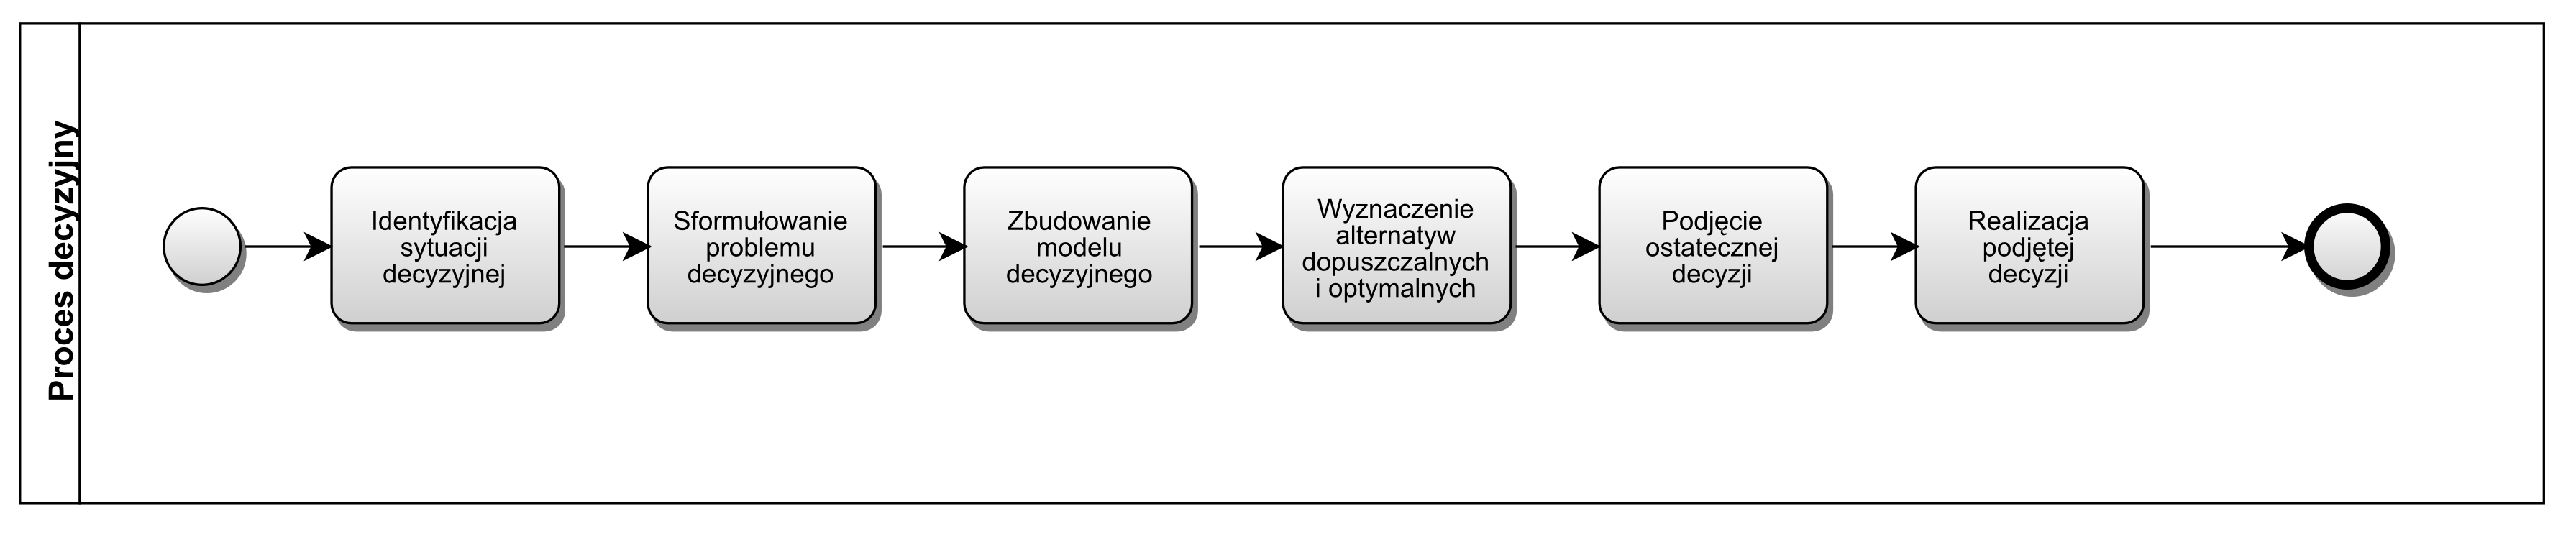
\includegraphics[scale=0.52]
  {chapters/decisiontheory/proces_decyzyjny}
  \caption{Proces decyzyjny}
  \label{fig:proces_decyzyjny}
\end{figure}

\subsection{Metody}
Teoria decyzji nie jest jednolitą dziedziną nauki, a raczej zbiorem 
wypracowanych metod przez różne dziedziny. Omawiając metody stosowane w teorii 
decyzji, nie można zapominać o jej interdyscyplinarnym charakterze. Stosując 
modele matematyczne, jak na przykład metody programowania liniowego, nie 
powinno się przesłaniać psychologicznych i socjologicznych aspektów procesu 
decyzyjnego.

Metody podejmowania decyzji dzielone są na kategorie. Jedną z tych kategorii 
jest omówione wcześniej podejście normatywne. Jeżeli decyzja podejmowana jest w 
warunkach pewności to mówi się o deterministycznych metodach teorii decyzji, 
natomiast ryzykiem i niepewnością zajmują się metody niedeterministyczne. 
Przypadkami kiedy jest więcej niż jedno kryterium oceny decyzji, zajmuje się 
dział zwany wielokryterialną analizą decyzyjną.

Podejście deskryptywne jest kolejną kategorią metod teorii decyzji. Podejście 
deskryptywne zajmuje się opisem typowych zachowań ludzi w procesie decyzyjnym i 
wskazuje na czynniki mające wpływ na podjęcie ostatecznej decyzji. Dlatego 
wyróżnia się tutaj metody psychologiczne oraz socjologiczne, na przykład 
negocjacje.

Ważnym rodzajem metod teorii decyzji jest komputerowe wspomaganie decyzji. 
Rozwój technologii informatycznych spowodował, że systemy komputerowe zaczęły 
pełnić istotną rolę tam, gdzie trzeba przetworzyć szybko bardzo dużą ilość 
danych, wykorzystać skomplikowane obliczeniowo modele albo, w przypadku grup, 
nie ma możliwości spotkania się w jednym miejscu w jednym czasie.

\section{Interdyscyplinarność}
Nowoczesna teoria decyzji zaczęła się rozwijać od połowy dwudziestego wieku z 
wielu dyscyplin naukowych. Chociaż obecnie jest to w dużej części dziedzina 
ścisła, to zazwyczaj jest realizowana przez naukowców z zakresu ekonomii, 
psychologii, nauk politycznych i społecznych, socjologów i psychologów. 
Istnieją pewne podziały prac pomiędzy tymi grupami. Politolog będzie studiował 
zasady głosowania oraz inne aspekty grupowego podejmowania decyzji. Psycholog 
oraz socjolog może badać zachowania osób podejmujących decyzje, a filozof 
wymagania dotyczące racjonalności. Matematyk opisze cały proces w sposób 
formalny, a informatyk zbuduje system w oparciu o ten model.

Mimo szerokiego pola badań, istnieje duża zbieżność co do podejścia do problemu.
Naukowcy z różnych środowisk wykorzystują wyniki badań z wszystkich dziedzin i 
stosują je przy rozwiązywaniu tych samych lub podobnych problemów. Teorię 
decyzji można rozpatrywać pod kątem jednej dyscypliny niezależnie, jednak 
najlepsze wyniki, najbardziej zbliżone do rzeczywistości, uzyskiwane są po 
uwzględnieniu osiągnięć wszystkich dziedzin zajmujących się teorią decyzji.


	
	\chapter{Grupowe podejmowanie decyzji}
	W teorii decyzji wyróżnia się gałąź, która zajmuje się problemem podjęcia
decyzji w przypadku, kiedy mamy do czynienia z większą niż jednoosobową grupą
ludzi, tak zwanych ekspertów. W takiej sytuacji zawodzą techniki znane  z
klasycznej teorii decyzji. Trzeba wziąć pod uwagę różne charaktery osób, ich
intencje oraz interesy.

Poniższy rozdział poświęcony jest psychologicznym aspektom grupy, wadom oraz 
zaletom grupowego podejmowania decyzji, jak również omówiony jest klasyczny
wyidealizowany model matematyczny, który stanowi podstawę dalszych rozważań.
Omówione też są strategie wykorzystywane w prawdziwym życiu przez grupy do
osiągnięcia porozumienia, czyli konsensusu.

Należy podkreślić, że omawiane decyzje grupowe nie są decyzjami związanymi z
polityką oraz wyborami demokratycznymi, bowiem te rządzą się innymi prawami. Tak
samo omawiane rodzaje grup dotyczą małej ilości ekspertów, od kilku do
kilkunastu osób.
\section{Charakterystyka grupy}

\subsection{Definicja grupy}
W teorii grupowego podejmowania decyzji można wyróżnić co najmniej trzy sposoby 
postrzegania grupy:
\begin{enumerate}

\item Grupa jako zbiorowa całość, jednostka niezależna od cech członków

\item Grupa jako zbiór jednostek, gdzie cechy grupy są funkcją cech
poszczególnych członków

\item Grupa jako zbiorowa całość, którą tworzy zestaw jednostek, gdzie
zrozumienie zachowań grupy wymaga zrozumienia jednocześnie cech grupy i cech
poszczególnych członków [Delbecq]

\end{enumerate}
Trzeci sposób jest najbardziej złożony i oddaje rzeczywisty obraz grupy. Analiza
tej perspektywy pozwala lepiej zrozumieć jej działanie, a dzięki temu lepiej ją
wspierać w procesie podejmowania decyzji. Należy pamiętać, że grupę tworzą
ludzie. Człowiek jest z natury istotą społeczną, chętną do pracy grupowej w
mniejszym lub większym stopniu. Jednocześnie każdy chce zachować swoją
indywidualność i niepowtarzalność.

Zgodnie z tymi rozważaniami grupa ma własny umysł i można badać jej zachowanie
niezależnie od badania cech jej członków, ale nie w oderwaniu od nich. Koncepcję
umysłu grupowego rozwinął D.M. Wegner, wprowadzając pojęcie systemu pamięci
transakcyjnej. Według niego pamięć transakcyjna jest właściwością grupy i nie
można jej przypisać żadnej pojedynczej jednostce, ani też znaleźć gdzieś między
członkami.

\begin{quote}\em
,,The transactive memory system in a group involves the operation of the 
memory systems of the individuals and the processes of communication that occur 
within the group. Transactive memory is therefore not traceable to any of the 
individuals alone, nor can it be found somewhere `between' individuals. Rather 
it is a property of a group.'' [1]
\end{quote}

\subsection{Koncepcja grup decyzyjnych}
W literaturze dotyczącej grupowego podejmowania decyzji rozważa się z reguły
grupę interaktywną. Można jednak wyróżnić co najmniej dwa inne typy zbiorowych
jednostek decyzyjnych. Nie są to grupy w potocznym rozumieniu, natomiast należy
je uznać za część procesu podejmowania decyzji grupowej, który będzie rozważany
później.
\begin{enumerate}[1)]
  \item Grupa interaktywna
  
  Tradycyjna grupa, której spotkanie rozpoczyna się od przedstawienia problemu
  przez przywódcę. Następnie ma miejsce niesformalizowana dyskusja służąca
  zgromadzeniu informacji na temat problemu i poznaniu stanowisk uczestników.
  Decyzja jest zwykle podejmowana przez głosowanie lub aklamację.

  \item Grupa nominalna
  
  Grupa nominalna jest to technika opracowana przez A. L. Delbecg i A. H. Van de
  Ven w 1968 roku (2). Procedura ma konkretną strukturę i przebiega w
  następujący sposób: 1) członkowie grupy w samotności spisują swoje pomysły,
  rozwiązania problemu lub realizacji zadania, 2) następnie w rundach każdy
  uczestnik przedstawia swoje pomysły, których podsumowanie jest bez dyskusji
  zapisywane na tablicy, 3) po przedstawieniu wszystkich pomysłów następuje
  dyskusja w celu omówienia i oceny zapisanych pomysłów, 4) na koniec członkowie
  ponownie w samotności dokonują oceny poprzez uszeregowanie wszystkich
  pomysłów. Decyzja „grupowa” wynika z agregacji indywidualnych pomysłów.

  \item Grupa delficka
  
  Członkowie grupy delfickiej, w przeciwieństwie do grup
  interaktywnych i nominalnych, fizycznie znajdują się w różnych miejscach i
  nie mają możliwości spotkania się twarzą w twarz w celu podjęcia decyzji.
  Grupa delficka wykorzystywana jest do uzgodnienia wspólnej opinii ekspertów. 
  Istotą techniki delfickiej jest korespondencyjne zbieranie pomysłów i opinii 
  na dany temat w ramach wybranej grupy społecznej lub zawodowej lub w ramach 
  wąskiej grupy ekspertów z konkretnej dziedziny. Badania te są najczęściej 
  przeprowadzane za pomocą ankiet przesyłanych drogą pocztową lub elektroniczną,
  ale możliwe są również badania o charakterze bardziej interaktywnym, np.
  z wykorzystaniem  komputerowych list dyskusyjnych. Następnie każdemu z
  ekspertów przesyłane są informacje o pomysłach pozostałych, anonimowych 
  uczestników w celu ich przeanalizowania i ewentualnej syntezy lub rewizji 
  swoich poglądów. Proces taki, w zależności od potrzeb można powtarzać 
  wielokrotnie.\todo{bibliografia}

\end{enumerate}


\subsection{Charakterystyka grup decyzyjnych}
Wszystkie wyżej wymienione rodzaje grup należy w jakiś sposób scharakteryzować. 
Harrison [3] zaproponował charakterystykę grup ze względu na trzy „kategorie”: 
kryteria oceny decyzji grupowej, sytuacyjne cechy grupowego podejmowania decyzji
oraz członkostwo grupowe.

\begin{itemize}
  \item Kryteria oceny decyzji grupowej
  
  Każda podjęta decyzja musi zostać poddana ocenie według pewnych przyjętych
  kryteriów.
  Do najważniejszych zaliczane są:
  \begin{itemize}
    \item jakość, 
    \item akceptacja, 
    \item oryginalność;
  \end{itemize}
  
  \item Sytuacyjne cechy grupowego podejmowania decyzji
  
  Za szczególnie ważne dla funkcjonowania grupy i dokonania przez nią wyboru
  uznaje się:
  \begin{itemize}
    \item dostęp do wiedzy fachowej,
    \item zasięg podmiotowy decyzji,
    konflikt w obrębie grupy;
  \end{itemize}
  
  \item Członkostwo grupowe
  
  Można przyjąć, że w skład grupy decyzyjnej wchodzą w różnych proporcjach trzy
  typy jednostek:
  \begin{itemize}
    \item ekspert,
    \item przedstawiciel,
    \item współpracownik.
  \end{itemize}
\end{itemize}

\begin{table}[t]
\caption{Charakterystyka grup decyzyjnych}
\begin{tabular}{|$>{\em}p{3cm}|^c|^c|^c|}
\hline
\rowstyle{\bfseries}
& Grupa interaktywna & Grupa nominalna & Grupa delficka \\
\hline
\hline
\multicolumn{4}{|l|}{\textbf{Kryteria oceny decyzji grupowej}} \\
\hline
\hline
jakość & średnia do wysokiej & średnia & niska do średniej \\
\hline
akceptacja & średnia do wysokiej & średnia & niska do średniej \\
\hline
oryginalność & niska do średniej & średnia & średnia do wysokiej \\
\hline
\hline
\multicolumn{4}{|l|}{\textbf{Sytuacyjne cechy grupowego podejmowania decyzji}}
\\
\hline
\hline
dostęp do wiedzy fachowej & niski do średniego & średni & średni do  wysokiego
\\
\hline
zasięg decyzji & średni do szerokiego & średni & wąski do średniego \\
\hline
konflikt w obrębie grupy & średni do wysokiego & niski do średniego & niski \\
\hline
\hline
\multicolumn{4}{|l|}{\textbf{Członkostwo grupowe}} \\
\hline
ekspert & okazjonalnie & często & zwykle \\
\hline
przedstawiciel & często & okazjonalnie & rzadko \\
\hline
współpracownik & zwykle & często & okazjonalnie \\
\hline

\end{tabular}

\label{tab:charakterystyka_grup}
\end{table}

\section{Strategie podejmowania decyzji}
W literaturze wymienia się trzy strategie (typy) grupowego podejmowania decyzji:
\begin{enumerate}[1)]
  \item rutynowe podejmowanie decyzji,
  \item twórcze podejmowanie decyzji,
  \item negocjacyjne podejmowanie decyzji.
\end{enumerate}

To, którą strategię wybierze grupa zależy od rodzaju podejmowanej decyzji. 
Strategia pierwsza dotyczy podejmowania programowanych decyzji, natomiast druga
- nieprogramowanych. Na każdą z trzech strategii grupowego podejmowania decyzji 
składa się zachowanie grupowe, które sprowadza się do pięciu wymiarów:
\begin{enumerate}[1)]
  \item struktura grupy,
  \item role grupowe,
  \item proces grupowy,
  \item styl grupowy,
  \item normy grupowe.
\end{enumerate}

Zależności zachowania grupy od przyjętej strategi zostały zaprezentowane w 
tabeli \ref{tab:Strategie_grupowego_podejmowania_decyzji}(źródło Harrison, s.
234).

\begin{table}[h]
\caption{Strategie grupowego podejmowania decyzji}
\begin{tabular}{|$m{1,8cm}|^m{4cm}|^m{4cm}|^m{4cm}|}
\hline
\rowstyle{\bfseries}
 & Rutynowe podejmowanie decyzji 
 & Twórcze podejmowanie decyzji 
 & Negocjacyjne podejmowanie decyzji 
 \\
 \hline
 \hline
\textbf{Struktura grupy}
& Specjaliści wraz z koordynatorem (przywódcą)
& Heterogeniczny, kompetentny skład; sprzyjający procesom twórczym kierownik
& Proporcjonalna reprezentacja zainteresowanych stron
\\
\hline
\textbf{Role grupowe} 
& Niezależny wysiłek; specjalistyczna wiedza 
& Wszystkie pomysły są przedmiotem grupowej dyskusji 
& Jednostka postrzega się jako reprezentant zainteresowanej strony 
\\
\hline
\textbf{Proces grupowy} 
& Określenie celów; interakcje pomiędzy koordynatorem i specjalistami 
& Proces rozwiązywania problemu z pełną partycypacją i spontaniczną komunikacją 
& Uporządkowana komunikacja; sformalizowane procedury obrad i głosowania 
\\
\hline
\textbf{Styl grupowy} 
& Znaczny stres wynikający z wymagań jakościowych i ilościowych oraz ograniczeń 
czasowych 
& Relaksacyjne, niestresujące otoczenie; brak sankcji 
& Otwartość i szczerość; Akceptacja procedur; unikanie wrogości
\\
\hline
\textbf{Normy grupowe} 
& Profesjonalizm 
& Otwartość komunikacji; konsensus; wspieranie oryginalności; eliminacja 
autorytaryzmu 
& Pragnienie osiągnięcia porozumienia; konstruktywne postrzeganie konfliktu; 
akceptacja kompromisu
\\
\hline
\end{tabular}

\label{tab:Strategie_grupowego_podejmowania_decyzji}
\end{table}

\section{Pułapki procesu decyzyjnego}
Proces formułowania i rozwiązywania problemu jest psychologicznie skomplikowany
i sprzyja powstawaniu wielu pułapek, w które wpada grupa. Ma to miejsce
szczególnie w przypadku grup niedoświadczonych, nieumiejętnie prowadzonych, ale 
również w przypadku osób, które mają już za sobą rozwiązanych wspólnie wiele 
problemów i podjętych decyzji.
Do najbardziej znanych problemów należą:
\begin{enumerate}
  \item Dysonans poznawczy
  
  Pojawia się wtedy, gdy występuje niezgodność pomiędzy przynajmniej dwoma
  przekonaniami. Teoria dystansu poznawczego stwierdza, że ludzie postępują
  rożnie w zależności od własnej samooceny. Osoby o wysokiej samoocenie po
  podjęciu decyzji podwyższają wartość wybranego rozwiązania jednocześnie
  dyskredytując pozostałe opcje. Osoby o niskiej samoocenie postępują odwrotnie
  - zaniżają wartość wybranego przez siebie sposobu działania. W praktyce
  oznacza to, że podjęcie decyzji może być pozorowane. Informacje oraz doradcy
  dobierani są selektywnie, aby usprawiedliwić wybór wariantu dokonany na
  początku. Dodatkowo osoby o niskiej samoocenie przez swoje niezdecydowanie
  mogą prowadzić proces w nieskończoność. Wszystko to prowadzi do podejmowania
  decyzji niezgodnej z opinią grupy, co nasila uczucie dysonansu.

  \item Iluzje decyzyjne
  
  Redukują nasz wysiłek i polegają na iluzorycznej pewności reguły decyzyjnej.
  Wyróżnia się cztery rodzaje iluzji:
  \begin{itemize}
    \item iluzja ekstrapolacji polegająca na założeniu, że dotychczasowe
    rozwiązania są skuteczne, co prowadzi do ich powielania bez względu na ich
    skuteczność w nowych warunkach;
    
    \item iluzja optymizmu, tzw. Monte Carlo, polegająca na uznawaniu, że
    zdarzenia cenne są bardziej prawdopodobne i po serii niepowodzeń wzrasta
    szansa sukcesu;
    
    \item iluzja Kolumba polegająca na tendencyjnym doborze i selekcji
    informacji w celu uzasadnienia wybranego rozwiązani;
    
    \item iluzja kontroli polegająca na wierze w możliwość kontrolowania zdarzeń
    losowych (jeśli lekko rzucimy kostką to wypadnie mała liczba, a jeśli mocno
    to duża).
  \end{itemize}
  
  \item Syndrom grupowego myślenia [4]
  
  Inaczej iluzja jednomyślności, jednak ze względu na powszechność tego zjawiska
  rozpatrywane jest jako osobna pułapka. Pojawia się gdy dążenie grupy do 
  konsensusu i jednomyślności przeważa nad dążeniem do osiągnięcia jak 
  najlepszej decyzji. W wyniku tego zjawiska może dojść do podjęcia decyzji 
  która nie leży w interesie grupy, ale jest sposobem na uniknięcie konfliktu.

\end{enumerate}

\section{Syndrom grupowego myślenia}
Termin ten został wprowadzony przez amerykańskiego psychologa Irvinga Janisa w
1972 roku. Udokumentowanym przykładem tego syndromu była katastrofa promu
kosmicznego ,,Challanger''. Podczas przygotowań do wystrzelenia wahadłowca
wystąpiło wiele problemów oraz pojawiły się liczne wątpliwości. Mimo tego na
każdym  etapie przygotowań podejmujący decyzje twierdzili, że nie ma podstaw do 
opóźnienia bądź odwołania startu.
Według Janisa [5] grupowe myślenie charakteryzuje się następującymi objawami:

\begin{itemize}
  \item iluzja nieomylności i pewności siebie,
  \item lekceważenie niepomyślnych informacji,
  \item lekceważące traktowanie wyników i osób spoza zespołu,
  \item wywierania nacisku dla wymuszenia konformizmu,
  \item samocenzurowanie się (aby uniknąć powtarzających się negatywnych reakcji
  grupy jej krytyczni członkowie decydują się milczeć),
  \item iluzja jednomyślności (milczenie jest oznaką zgody),
  \item filtrowanie informacji, czyli niedopuszczanie danych sprzecznych ze
  zdaniem grupy.
\end{itemize}

Grupa widzi i słyszy tylko to, co chce. Nie poszukuje się i nie bierze pod uwagę 
nowych możliwości, co prowadzi do podejmowania błędnych decyzji. Według Janisa, 
aby skutecznie funkcjonować, grupa musi ciągle pobierać i odpowiednio
weryfikować uzyskane informacje. Proces ten może ulegać defektom prowadzącym do
błędnych decyzji. Najważniejsze defekty to:

\begin{itemize}
  \item ograniczenie dyskusji do rozważania zaledwie kilku działań bez
  analizowania pełnej gamy alternatyw,
  \item unikanie przez grupę powtórnego analizowania poprzednio preferowanego
  sposobu działania,
  \item lekceważenie alternatyw początkowo ocenionych negatywnie,
  \item bardzo małe wykorzystanie możliwości uzyskania informacji od
  zewnętrznych ekspertów.
\end{itemize}

Aby uniknąć wystąpienia grupowego myślenia, każdy członek grupy powinien
wnikliwie i krytycznie ocenić wszystkie możliwe rozwiązania. Przywódca nie
powinien zbyt wcześnie wygłaszać swojego poglądu, aby wszyscy członkowie grupy
mieli szanse wypowiedzieć się swobodnie. Syndrom grupowego myślenia zrobił duża
karierę w psychologii społecznej, należy jednak pamiętać, że posiada niewielkie
osadzenie w systematycznych badaniach naukowych. Został sformułowany na
podstawie obserwacji kilku spektakularnych, błędnych decyzji podejmowanych przez
wybitnych specjalistów.

\section{Zalety i wady}
Powszechnie przyjmuje się, że ,,co dwie głowy to nie jedna''. Teoretycznie
decyzje podjęte przez grupę ekspertów wskutek kumulacji wiedzy wielu jednostek 
powinny stanowić najlepsze z możliwych rozwiązań omawianego problemu, powinny
być lepiej przemyślane oraz bardziej różnorodne niż w przypadku decyzji
jednoosobowej. Niestety, jak pokazano wcześniej, grupa narażona jest na szereg
pułapek i błędów, które może popełnić jeżeli jest źle dobrana bądź
nieodpowiednio moderowana.

\subsection{Zalety}
Jako zalety przemawiające za podjęciem decyzji grupowo wymienia się: [1]
\begin{enumerate}

  \item Większą ogólną sumę wiedzy lub informacji.
   
   Grupa dysponuje większą ilością informacji niż którykolwiek z jej członków.
   Dlatego w sytuacjach wymagających wiedzy decyzje grupowe powinny być lepsze
   od indywidualnych.
   
   \item Większą ilość podjeść do problemu.
   
   Jednostki często myślą w sposób rutynowy, natomiast konfrontacja z innymi
   osobami o odmiennych punktach widzenia stymuluje nowe poglądy i poszerza
   indywidualne horyzonty.
   
   \item Zwiększona ogólna akceptacja końcowego wyboru.
   
   Kiedy decyzję podejmuje grupa, większa liczba osób odczuwa i akceptuje
   odpowiedzialność za realizację wybranego kierunku działania. Co więcej,
   akceptowana decyzja o niskiej jakości może okazać się bardziej efektywna od
   decyzji o wysokiej jakości, która nie cieszy się poparciem.
   
   \item Lepsze zrozumienie decyzji
   
   Udział w podejmowaniu decyzji ułatwia komunikację w trakcie jej realizacji.

\end{enumerate}

\subsection{Wady}
Jako wady przeszkadzające grupie w dokonaniu optymalnej decyzji wymienia się:
\begin{enumerate}
  \item Nacisk społeczny
  
  Dążenie do tego, aby być dobrym członkiem członkiem grupy i akceptowanym przez
  nią sprzyja konsensusowi i łagodzi nieporozumienia. Niestety nacisk na grupową
  spójność i jednomyślność może prowadzić do wspomnianego wcześniej syndromu
  myślenia grupowego.
  
  \item Akceptacja pierwszego rozwiązania
  
  Bardzo często grupa akceptuje pierwsze rozwiązanie, które cieszy się silnym
  poparciem większości członków lub dominującej mniejszości. Zgłoszone później
  lepsze alternatywy mają niewielką szansę na dokładną analizę i uwzględnienie.
  
  \item Dominacja jednostki
  
  W większości grup wyznaczany jest przywódca albo wyłania się jednostka
  dominująca, która wywiera wpływ na pozostałych członków i niejako narzuca
  swoje zdanie. Dominacja jednego (lub kilku) członka grupy może spowodować
  wycofanie się pozostałych osób z aktywnego uczestnictwa i tym samym zatraca
  się idea grupowego podejmowania decyzji.
  
  \item Konkurencja między decyzjami
  
  Pojawienie się kilku alternatywnych kierunków działania często powoduje, że
  członkowie grupy dążą do wyboru zgodnego z ich preferencjami. Dominacja
  własnych preferencji nad dążeniem do znalezienia najlepszego rozwiązania
  prowadzi do kompromisowej decyzji o niskiej jakości.
  
  \item Czas potrzebny na proces decyzyjny
  
  ,,Gdyby Mojżesz miał radę doradczą to Izraelici po dziś dzień tkwiliby w
  Egipcie''. Jedna osoba jest w stanie podjąć samodzielną decyzję dużo szybciej
  niż grupa. Grupa musi się naradzić, przedyskutować wszystkie możliwości. 
  Jeśli ten proces nie jest odpowiednio moderowany to rozmowy mogą trwać w
  nieskończoność.

  \item Polaryzacja grupowa
  
  To tendencja grup do podejmowania decyzji bardziej skrajnych niż początkowo
  członkowie zakładali indywidualnie. Dla przykładu zdarza się, że rada
  przysięgłych w sądzie po dyskusji jest skłonna wydać wyrok znacznie wyższy lub
  niższy niż którykolwiek z członków proponował przed debatą.

\end{enumerate}

\section{Model klasyczny}
Według Roberta Harrisa podejmowanie decyzji to identyfikacja i wybór
alternatywnych rozwiązań w oparciu o wartości i preferencje decydentów. Z
podjęcia decyzji wynika fakt istnienia różnych alternatyw do rozważenia i w
takim przypadku należy nie tylko zidentyfikować jak najwięcej opcji, ale również
wybrać tą jedyną, która pasuje do naszych celów, pragnień, wartości i tym
podobnych. \todo{biblio}

W związku z powyższym można zdefiniować klasyczny i najprostszy proces 
podejmowania decyzji grupowej, jak również indywidualnej.
\begin{description}
  \item[Krok 1 - definicja problemu] Celem jest wyrażenie problemu w
  sposób jasny posługując się regułą ,,one-sentence problem'', czyli za pomocą
  jednego zdania, tak aby opisać zarówno warunki początkowe jak i pożądane
  efekty. Oczywiście limit „jedno zdanie” w praktyce zostanie w wielu
  przypadkach przekroczony, szczególnie w przypadku bardzo złożonych problemów 
  decyzyjnych. Mimo wszystko definicja problemu musi być zwięzła i uzgodniona
  przez wszystkich decydentów. Nawet jeśli może to być długi, iteracyjny proces,
  to jest to ważny i konieczny punkt przed przejściem do następnego kroku.
  
  \item[Krok 2 - określenie wymagań] Wymagania są to warunki, które wszystkie
  dopuszczalne rozwiązania problemu muszą spełniać. W postaci matematycznej, 
  wymagania to są ograniczenia określające zbiór możliwych (dopuszczalnych) 
  rozwiązań problemu decyzyjnego. Bardzo ważne jest, że nawet jeśli w kolejnych 
  krokach mogą wystąpić subiektywne lub sporne oceny to ewentualne rozwiązanie 
  musi być rozstrzygalne jednoznacznie, albo spełnia wymagania albo nie.
  
  \item[Krok 3 - ustanowienie celów] Cele wykraczają poza niezbędne minimum
  które musi spełniać rozwiązanie, czyli wymagania. Są to szeroko pojęte 
  potrzeby i pragnienia. Mogą być ze sobą sprzeczne, co jest naturalne w 
  praktycznych sytuacjach decyzyjnych.
  
  \item[Krok 4 - identyfikacja alternatyw] Alternatywy oferują różne podejścia
  zmiany stanu początkowego w stan pożądany. Są to możliwe rozwiązania 
  postawionego problemu, które bezwzględnie muszą spełniań zdefiniowane 
  wcześniej wymogi. Nie tracąc na ogólności w dalszych rozważaniach przyjmuje 
  się, że zbiór alternatyw jest skończony.
  
  \item[Krok 5 - zdefiniowanie kryteriów oceny] Kryteria decyzyjne, które będą
  dyskryminować alternatywy, muszą opierać się na celach. Konieczne jest 
  określenie kryteriów dyskryminacyjnych jako mierników sprawdzających w jakim 
  stopniu każda alternatywa osiąga cele. Wynika z tego, że każdy cel 
  reprezentowany jest formie kryteriów i każdy cel musi generować przynajmniej 
  jedno kryterium. W przypadku bardzo dużej ilości kryteriów pomocne jest 
  podzielenie ich w zestawy (na przykład tematyczne). Według Baker et al.
  [6] kryteria powinny być:
  
  \begin{itemize}
    \item w stanie dyskryminować alternatywy i wspierać ich porównywanie
	\item pokrywać wszystkie cele
	\item sensowne i operacyjne
	\item nieredundantne
	\item nieliczne
  \end{itemize}
  
  Warto wspomnieć, że niektórzy autorzy posługują się słowem atrybut, zamiast 
  kryterium. Atrybut jest czasem również używany do określenia wymiernego
  kryterium.
  
  \item[Krok 6 - wybór narzędzia wspierającego podejmowanie decyzji] 
  Obecnie dostępnych jest wiele narzędzi wspierających podejmowanie decyzji.
  Wiele z nich to na przykład materiały ułatwiające głosowanie lub usprawniające
  cały proces. Można też skorzystać z dostępnego oprogramowania, niestety w
  większości przypadków są to systemy płatne.
  \item[Krok 7 - ocena alternatyw względem przyjętych kryteriów] 
  Każda poprawna metoda podejmowania decyzji potrzebuje, jako dane wejściowe,
  metody oceny alternatyw względem kryteriów. W zależności od przyjętych
  kryteriów, ocena może być obiektywna, czyli odnosić się do powszechnie
  przyjętych i rozumianych skali pomiaru (np. pieniądze) lub subiektywna
  (sędzia), co odzwierciedla subiektywną ocenę decydenta. Po dokonaniu oceny,
  wybrane narzędzie podejmowania decyzji może uporządkować alternatywy lub
  wybrać podzbiór rozwiązań najbardziej obiecujących.
  \item[Krok 8 - weryfikacja rozwiązań względem postawionego problemu] 
  Zbiór alternatyw wybrany przez narzędzie zawsze musi zostać zweryfikowany pod
  kątem wymagań i celów problemu decyzyjnego. Zdarza się, że zostało wybrane
  niewłaściwe narzędzie. Może się również okazać, że decydenci mogą dodać lub
  zmieć cele i wymagania.

\end{description}





	
	\chapter{Modelowanie grupowego podejmowania decyzji}
	Proces podejmowania decyzji, polegający na wybieraniu najlepszej opcji z 
zestawu możliwych, jest obecny w niemal każdym możliwym zadaniu człowieka. Z
tego powodu, badania nad podejmowaniem decyzji są konieczne i ważne nie tylko w 
teorii decyzji, ale również w takich dziedzinach jak zarządzanie, badania
operacyjne,  polityka, psychologia społeczna, sztuczna inteligencja, soft 
computing i tak dalej. Oczywistym jest, że porównywanie różnych działań w 
zależności od ich zalet, w wielu przypadkach, jest niemożliwe do osiągnięcia 
przy pomocy jednego kryterium lub jednej osoby. Dlatego też, proces decyzyjny 
rozpatrywany jest jako grupowe podejmowanie decyzji.

Niezaprzeczalnym faktem jest, że problemy stawiane grupie w większości pochodzą 
z sytuacji z życia wziętych. W tych problemach jest do dyspozycji zbiór
alternatyw rozwiązujących problem oraz grupa ekspertów, cechująca się
doświadczeniem i wiedzą, która stara się osiągnąć wspólne rozwiązanie. Aby
rozwiązać problem, eksperci muszą przejść przez dwa etapy: proces osiągania
konsensusu oraz proces selekcji.

W poniższym rozdziale te dwa etapy zostaną dokładnie opisane. Przedstawiony
będzie model iteracyjny, który wykorzystuje proces osiągania konsensusu i proces
selekcji. Na końcu wprowadzone zostaną elementy dynamiki, które mogą pojawić się
w procesie podejmowania decyzji oraz propozycje poradzenia sobie z tym.

\section{Model iteracyjny}
W grupowym podejmowaniu decyzji można wyróżnić dwa procesy prowadzące do
uzyskania ostatecznego rozwiązania: proces osiągania konsensusu oraz proces
selekcji \cite{Herrera1996,Alonso2009}. Pierwszy zajmuje się osiągnięciem
maksymalnie najwyższego porozumienia pomiędzy ekspertami. Zwykle proces ten
prowadzony jest przez tak zwanego moderatora i jest wykonywany przed procesem
selekcji. Proces porozumienia jest bardzo ważnym krokiem, ponieważ wspomaga
uzyskanie rozwiązań o wysokim stopniu konsensusu wśród  ekspertów, co zazwyczaj
jest pożądaną własnością. Drugi proces odnosi się do sposobu uzyskania zbioru
alternatyw jako rozwiązań z opinii oraz ocen każdej z alternatyw przedstawionych
przez ekspertów.

\subsection{Definicja problemu}
Przed przystąpieniem do poszczególnych kroków trzeba formalnie zdefiniować 
problem. Z punktu widzenia modelu, nie jest to opis czy postawione pytanie. 
Typowy wieloosobowy, wielokryteriowy problem składa się z następujących 
elementów \cite{Ekel2009}:

\begin{description}
  \item[Zbiór alternatyw $ \mathcal{X} = \{ x_1, \dotsc, x_n \}.$] Zbiór
  $\mathcal{X}$ odpowiada skończonej i dyskretnej liście więcej niż jednej
  możliwości. Odpowiednie właściwości (lub atrybuty) każdej alternatywy mogą być
  ilościowe lub jakościowe.
  
  \item[Zbiór kryteriów $ \mathcal{C} = \{ c_1, \dotsc, c_n \}.$] Zbiór
  $\mathcal{C}$ zawiera dwa lub więcej kryteriów. Każdemu kryterium odpowiada
  punkt widzenia, zgodnie z którym alternatywy są oceniane i porównywane. Mogą
  one mieć charakter ilościowy lub jakościowy i posiadać większą lub mniejszą
  wagę dla decyzji.
  
  \item[Zbiór decydentów $ \mathcal{E} = \{ e_1, \dotsc, e_n \}.$] Zbiór
  $\mathcal{E}$ zawiera więcej niż jednego eksperta. Zazwyczaj każdy z ekspertów
  ma własną perspektywę, motywację i priorytety, które mogą prowadzić do
  sprzecznych opinii i preferencji. Ponadto każdy decydent odgrywa rolę w
  procesie decyzyjnym, która jest określana przez stopień wiedzy, doświadczenia
  oraz intuicji w danej sprawie.

\end{description}

\subsection{Proces porozumienia (konsensusu)}

\begin{figure}[ht]
  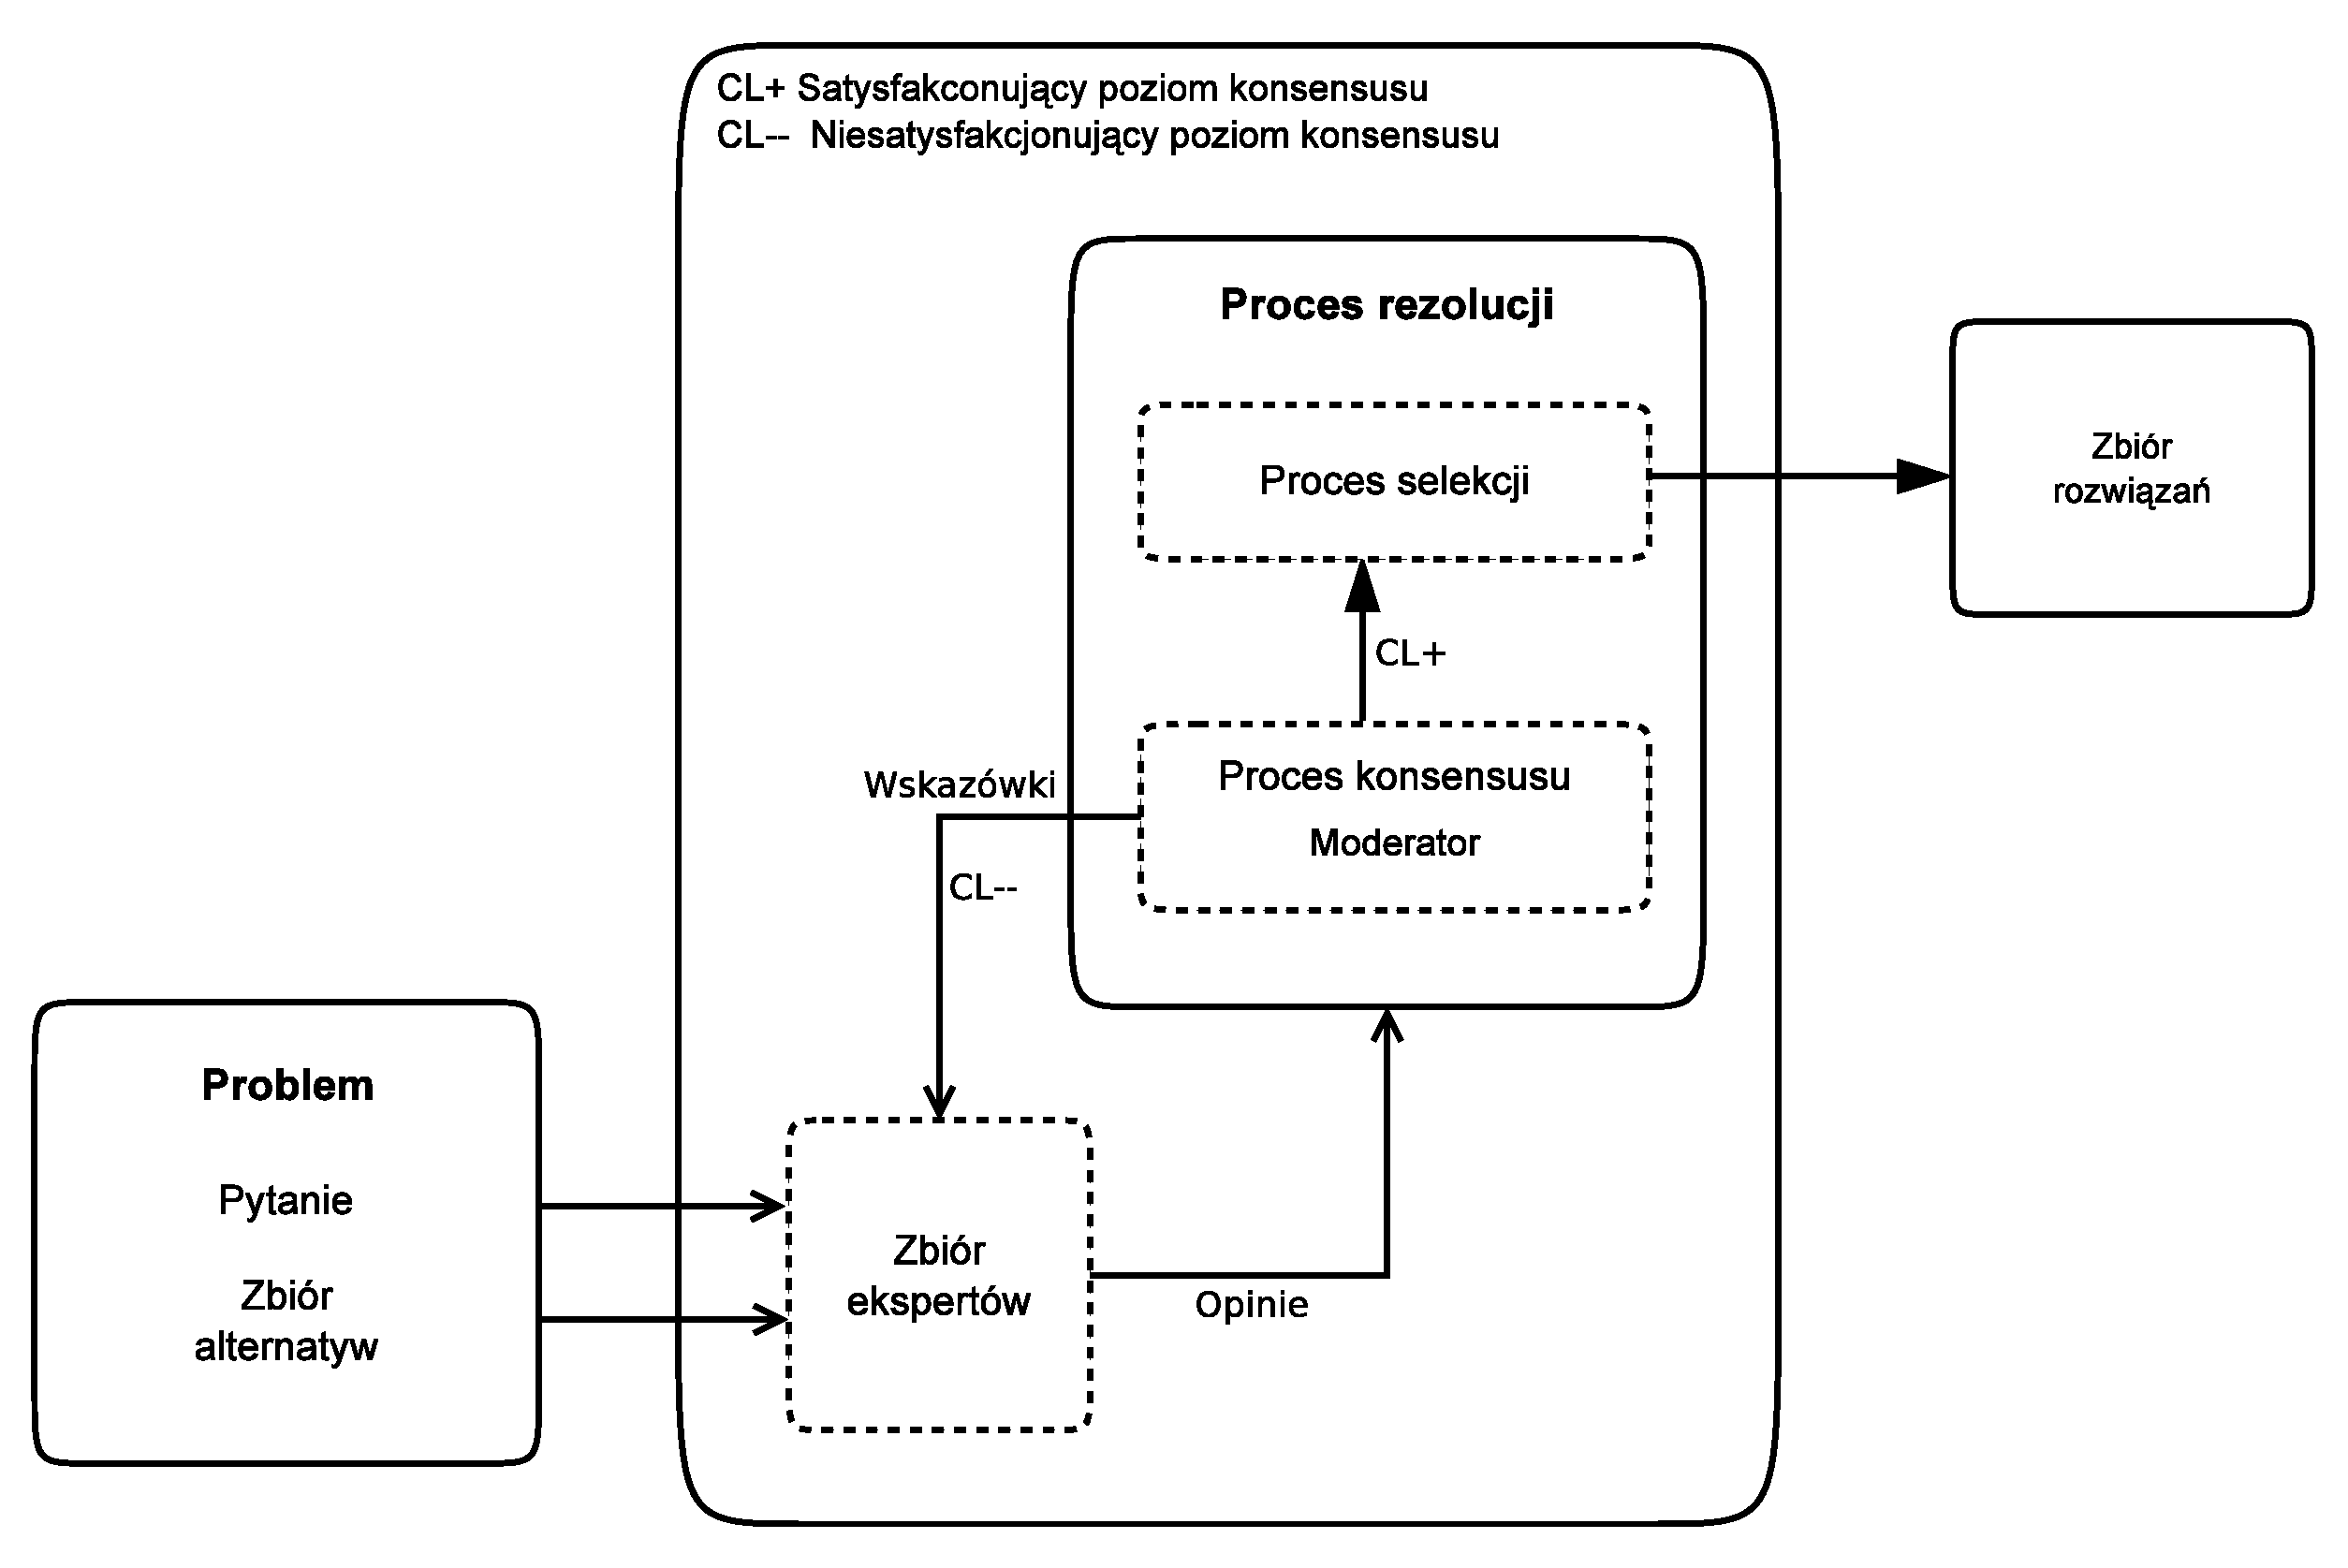
\includegraphics[width=\linewidth]
    {chapters/modelinggroupdecision/schemat_procesu-eps-converted-to.pdf}
  \caption{Procesy w grupowym podejmowaniu decyzji}
  \label{fig:Procesy_w_grupowym_podejmowaniu_decyzji}
\end{figure}

Typowy proces
porozumienia widoczny jest na rysunku
\ref{fig:Procesy_w_grupowym_podejmowaniu_decyzji}. Jest on zdefiniowany jako
dynamiczny proces iteracyjny i obejmuje następujący skończony zbiór kroków:
\begin{enumerate}[1.]
  \item Problem oraz zbiór możliwych alternatyw przedstawiane są ekspertom.
  
  \item \label{itm:2nd} Eksperci przedstawiają moderatorowi swoje preferencje
  przy użyciu określonego sposobu reprezentacji preferencji.
  
  \item Kiedy wszyscy przedstawią swoje preferencje, moderator sprawdza czy 
  poziom konsensusu wśród wszystkich ekspertów jest wystarczająco wysoki.
  
  \item 
  \begin{enumerate}[i)]
    \item Jeśli poziom konsensusu jest wystarczająco wysoki to proces się kończy
    i przechodzi do procesu selekcji (krok \ref{itm:6th}).
	\item Jeśli poziom konsensusu nie jest wystarczająco wysoki to moderator 
	udziela ekspertom wskazówek tak, aby mogli zmienić swoje preferencje i 
	osiągnąć konsensus.
  \end{enumerate}
  
  \item Biorąc pod uwagę zalecenia moderatora, eksperci zmieniają swoje
  preferencje co do alternatyw i rozpoczyna się nowa runda procesu (krok
  \ref{itm:2nd}).
  
  \item \label{itm:6th} Przejście do procesu selekcji i obliczenie
  ostatecznego rozwiązania.

\end{enumerate}

Warto zwrócić uwagę, że tak zdefiniowany proces konsensusu może przypominać 
klasyczną metodę delficką \cite{Helmer-Hirschberg1967}. Jednakże istnieje kilka
istotnych różnic:
\begin{itemize}
  \item W metodzie delfickiej ostatecznym celem jest prognozowanie, podczas gdy 
  powyższe podejście próbuje znaleźć najlepszą alternatywę z zestawu możliwych.
  \item Zamiast kwestionariuszy, eksperci wyrażają swoje preferencje za pomocą 
  pewnych konkretnych formatów reprezentacji preferencji.
  \item Metoda delficka zakłada anonimowość uczestników, natomiast w 
  proponowanym modelu nie ma takiego ograniczenia.
\end{itemize}

W przedstawionym modelu bardzo ważna jest rola moderatora. W dalszej części 
pracy zostaną przedstawione narzędzia pozwalające zredukować jego pracę, a 
nawet go zastąpić. Kolejnym ważnym elementem jest sposób przedstawienia 
preferencji ekspertów. Temu tematowi poświęcony jest osobny rozdział.

\subsection{Proces selekcji}
Etap ten na wejściu dostaje oceny wszystkich ekspertów i jest odpowiedzialny za 
podanie kolejności rozwiązań. Proces selekcji można różnie definiować, w 
zależności od dokładnego umiejscowienia w modelu oraz zakresu odpowiedzialności 
procesu konsensusu. Zgodnie z Chiclana et al. \cite{Chiclana1998,Chiclana2001}
proces selekcji jest podzielony na dwie fazy:
\begin{enumerate}
  \item Faza agregacji
  
  Faza ta definiuje globalne preferencje pomiędzy alternatywami wykorzystując 
  do tego techniki agregacji.
  
  \item Faza eksploatacji
  
  Faza ta przekształca zagregowaną globalną informację o preferencjach względem 
  alternatyw w globalny ranking. Sposób ustalenia rankingu jest dowolny i zależy
  od przyjętych technik reprezentacji preferencji i agregacji.

\end{enumerate}

\subsection{Moderator i mechanizm informacji zwrotnej}
Moderator jest osobą niebiorącą udziału w dyskusji w sposób bezpośredni. Jego
zadaniem jest kierowanie grupą, analizowanie wyników głosowań i na ich podstawie
wpływanie na na opinie ekspertów tak, aby został osiągnięty jak największy 
stopień konsensusu. Jako część modelu wprowadzony zostaje mechanizm informacji 
zwrotnej, który ma zastąpić osobę moderatora i zautomatyzować proces. Mechanizm 
składa się z kilku prostych zasad, które generują rekomendacje dla ekspertów. 
Aby to osiągnąć, wykorzystywane są miary przybliżone w połączeniu ze stopniem 
konsensusu \cite{Herrera1995}. Na końcu, porady muszą zostać przedstawione w
sposób czytelny dla człowieka, żeby eksperci mogli je wykorzystać do zmiany
swoich poglądów.

\section{Dynamika: zbiór alternatyw}
Zazwyczaj metody rozwiązywania problemów grupowych są statyczne
\cite{Perez2010}. Oznacza to założenie, że liczba alternatyw oraz ekspertów
przez cały proces decyzyjny jest stała. Jednak w rzeczywistych sytuacjach
okazuje się, że proces może być dynamiczny.

Szczególnie częstym zjawiskiem jest dynamika zbioru alternatyw. Typowym 
przykładem takiej sytuacji jest diagnoza lekarska. Środowisko to jest dynamiczne
w tym sensie, że pacjent może przedstawić nowe objawy lub mógł poczuć się lepiej
ze względu na przyjmowane leki, a więc każda zmiana stanu pacjenta powinna być 
brana pod uwagę przez lekarzy.

Aby proces decyzyjny stał się bardziej realistyczny, należy zdefiniować metodę, 
która pozwala usunąć i wstawić nowe alternatywy do procesu dyskusji. Ze względu 
na chęć wyeliminowania osoby moderatora, metoda ta powinna być maksymalnie 
zautomatyzowana.

\begin{figure}[ht]
  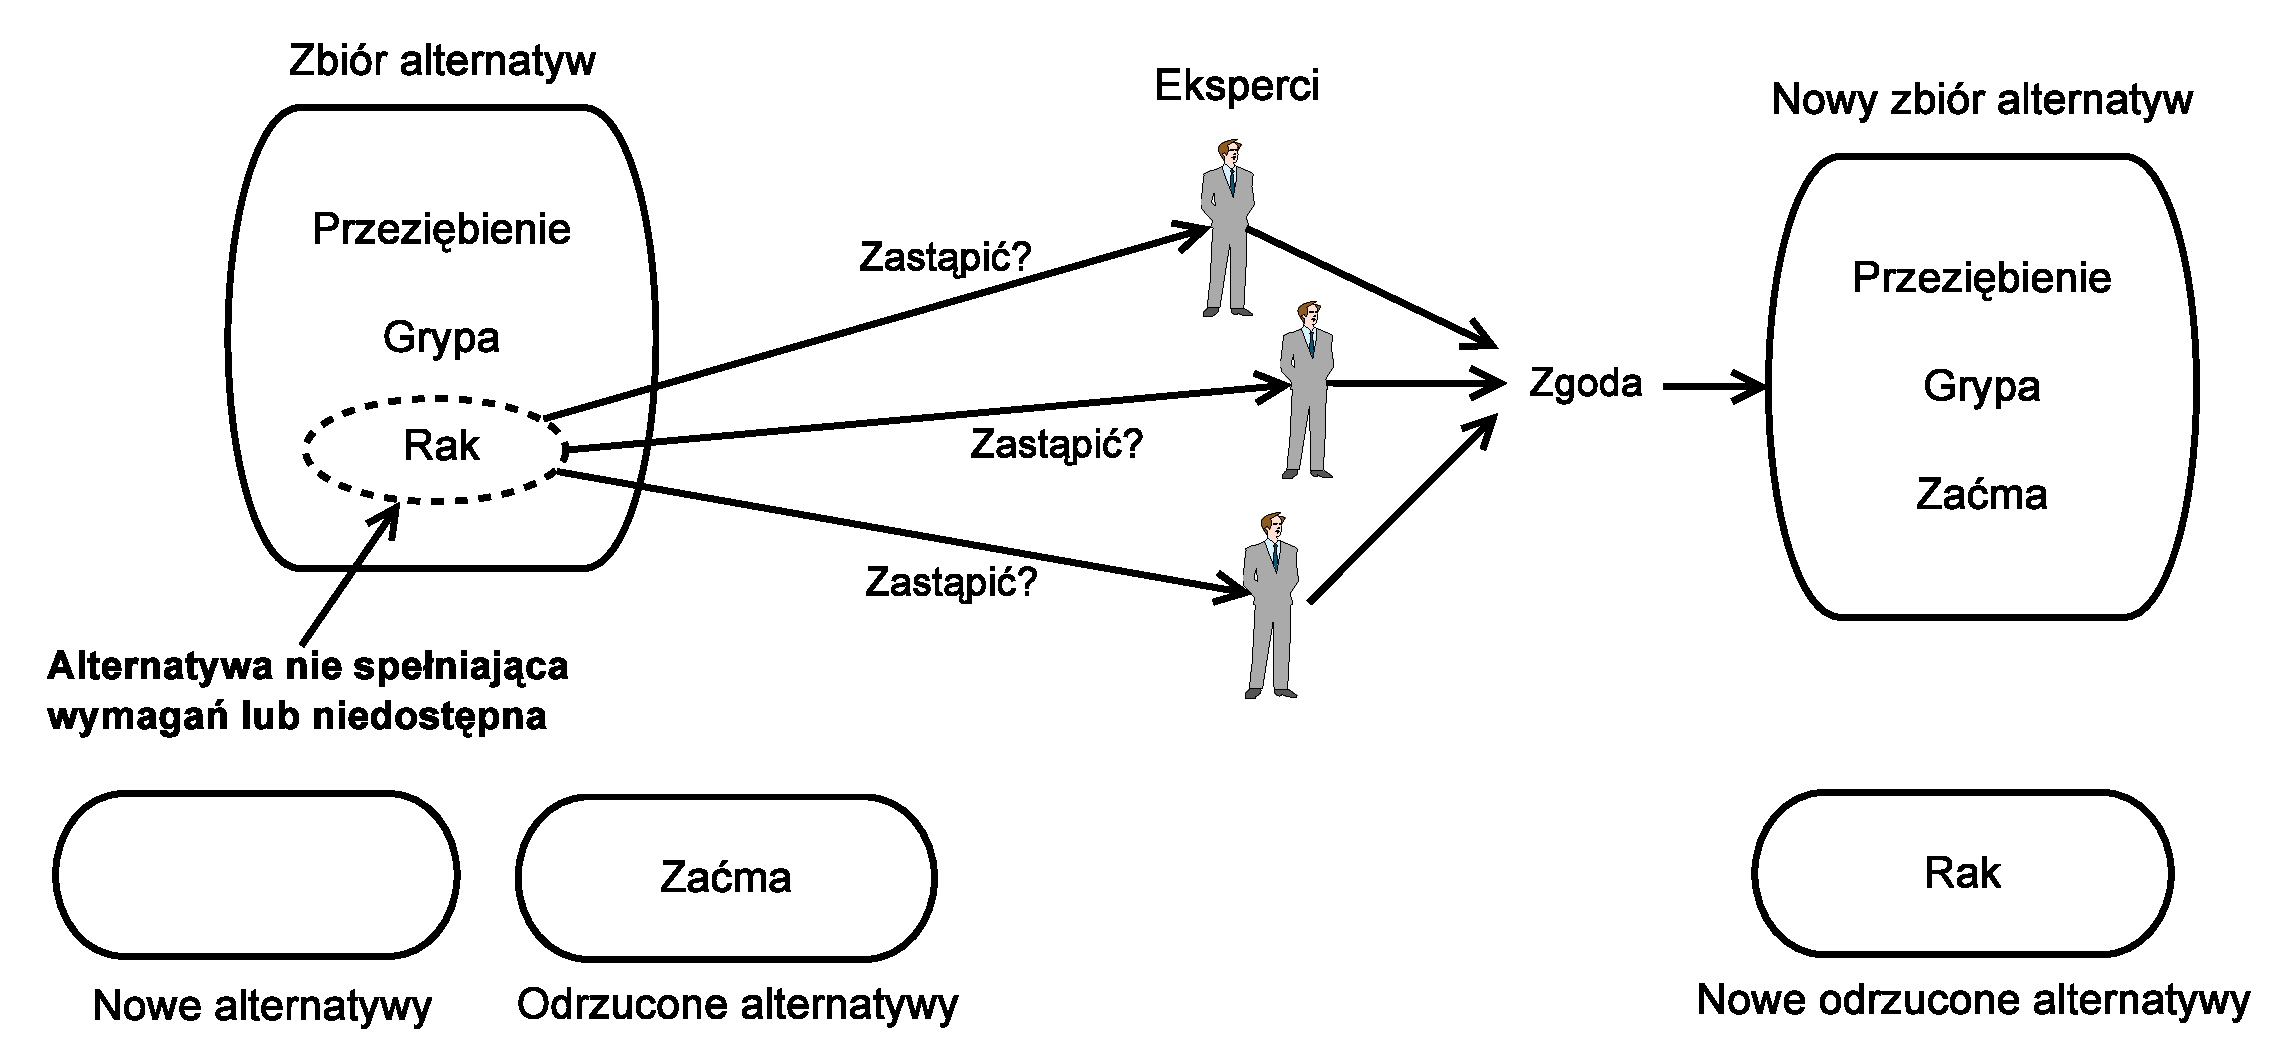
\includegraphics[width=\linewidth]
  	{chapters/modelinggroupdecision/usuniecie_alternatyw-eps-converted-to.pdf}
  \caption{Dynamika alternatyw: Usunięcie}
  \label{fig:dynamika_alternatyw_usuniecie}
\end{figure}

Wpierw, system identyfikuje rozwiązania najgorsze ze względu na oceny ekspertów,
które mogą zostać usunięte. Następnie szuka nowych, które może dołączyć. Nowe 
alternatywy można uzyskać z propozycji, które pojawiły się w trakcie dyskusji 
albo ze zbioru rozwiązań, które były dostępne od samego początku, ale nie 
zostały ujęte w dyskusji ze względu na nie spełnienie początkowych kryteriów 
problemu. Istnieje też możliwość ponownego włączenia do dyskusji alternatyw 
wcześniej usuniętych. Wyraźnie widać, że metoda dzieli się na dwie fazy: 
usunięcie nieaktualnych i złych alternatyw (rysunek
\ref{fig:dynamika_alternatyw_usuniecie}) oraz dodanie nowych alternatyw (rysunek
\ref{fig:dynamika_alternatyw_dodanie}).
W tak zdefiniowanej metodzie moderator jest zastąpiony przez system oraz samych
decydentów, którzy muszą być informowani o zmianach i je akceptować.

\begin{figure}[ht]
  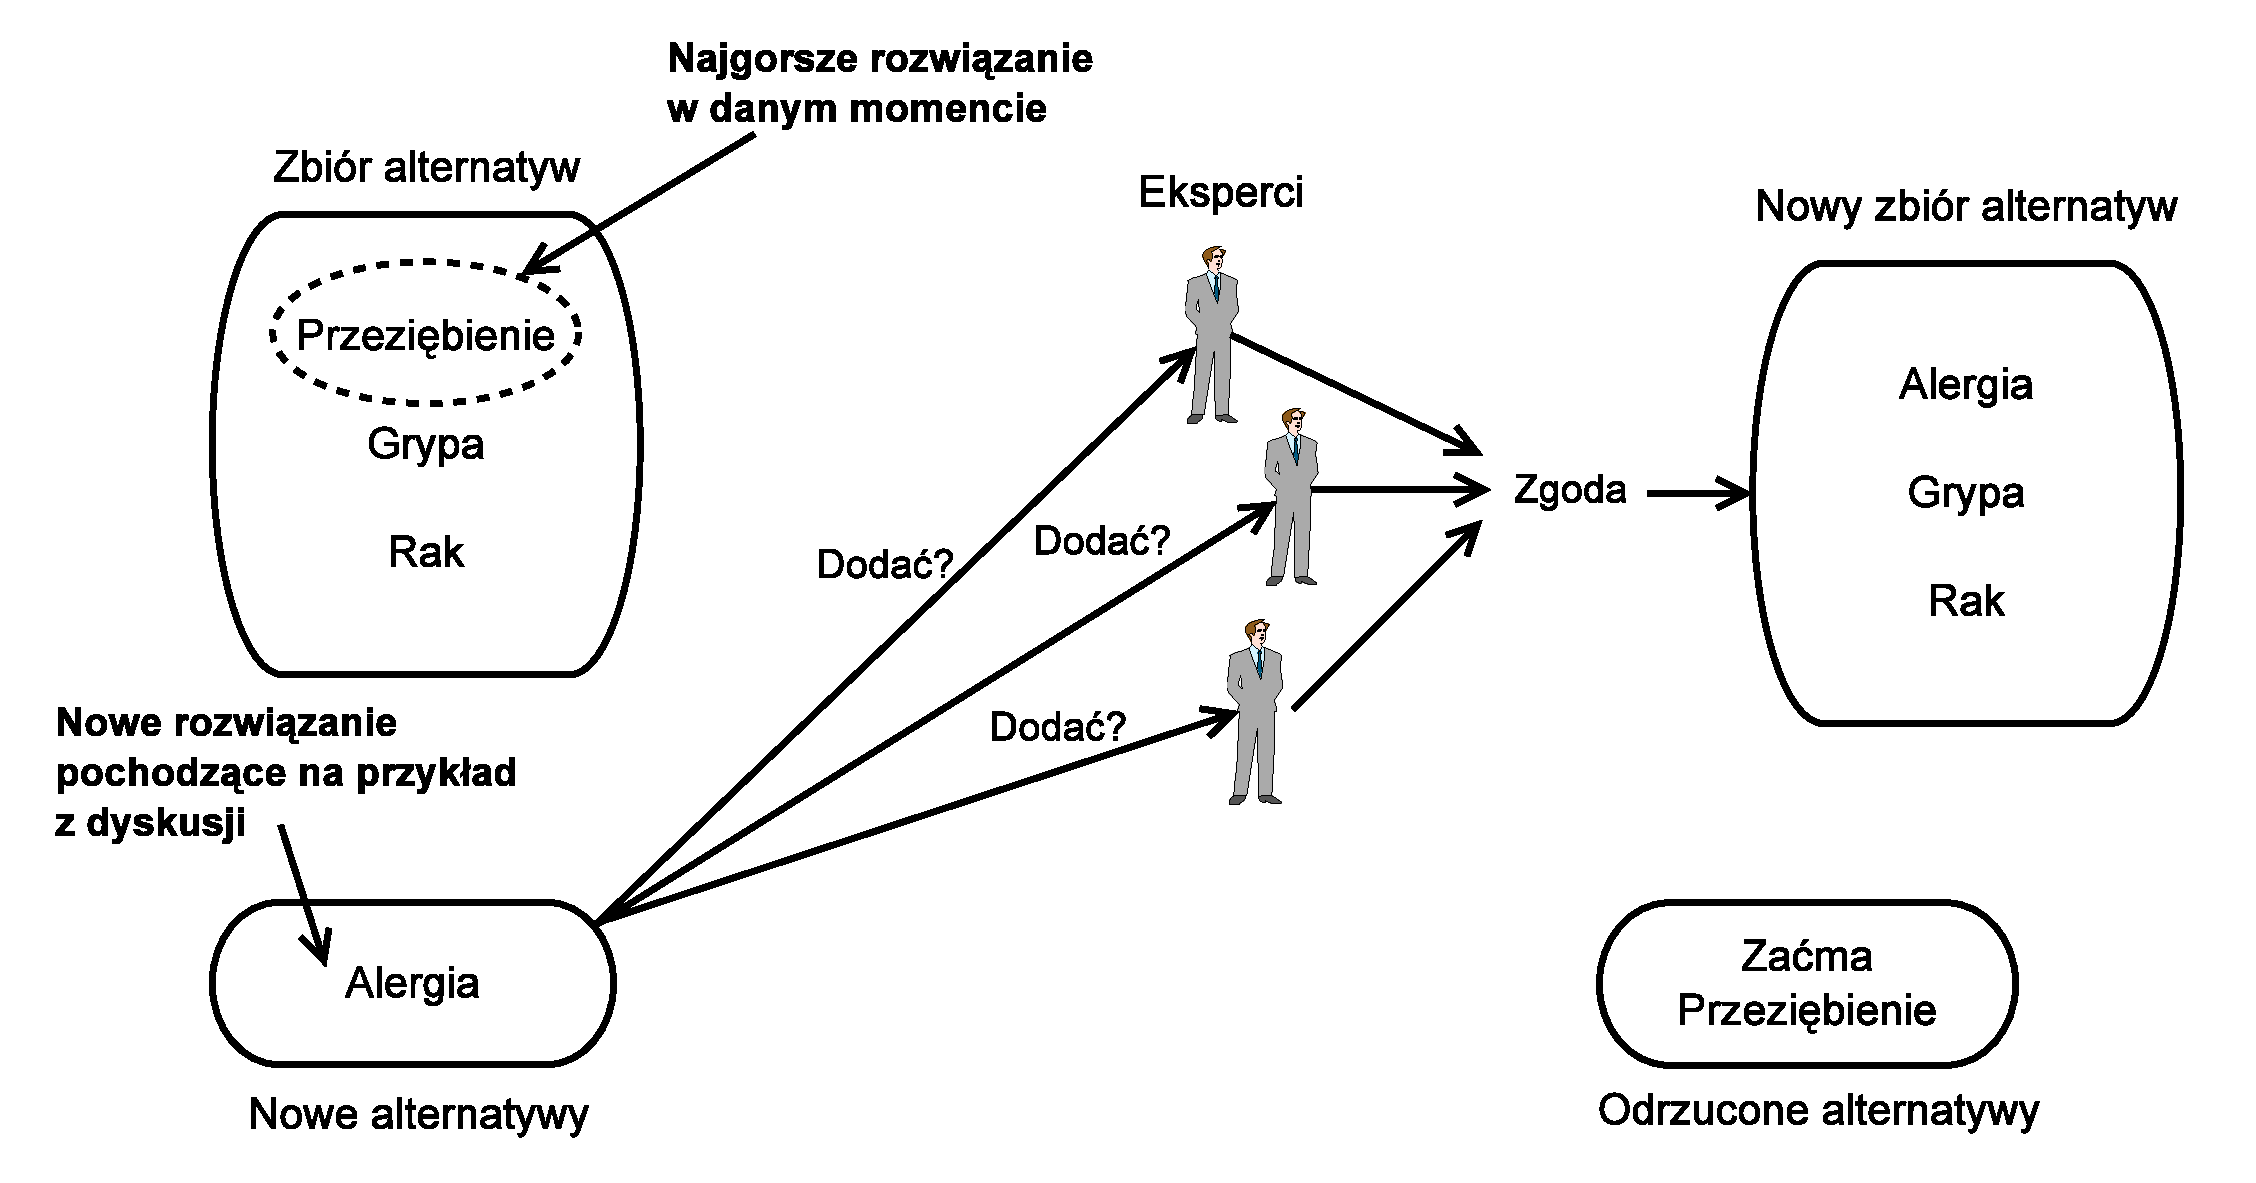
\includegraphics[width=\linewidth]
  	{chapters/modelinggroupdecision/dodanie_alternatyw-eps-converted-to.pdf}
  \caption{Dynamika alternatyw: Dodanie}
  \label{fig:dynamika_alternatyw_dodanie}
\end{figure}

\section{Dynamika: zbiór ekspertów}
Kolejnym aspektem jest dynamiczny zbiór ekspertów. Przykładem może być grupa
lekarzy, którzy na pewnym etapie badań nie są w stanie postawić diagnozy i
proszą o konsultację z innym lekarzem lub lekarzami, którzy mogą mieć większe
doświadczenie w danej dziedzinie. Innym przykładem jest sytuacja, w której
członek grupy decydentów w firmie przebywał na urlopie i wraca do pracy w
trakcie trwania procesu decyzyjnego. Może się również zdarzyć, że jeden z
członków odchodzi z zespołu lub na jakiś czas wyłącza się z dyskusji. Oba
przypadki, dodanie oraz usunięcie decydenta, powinny być wspierane przez system
podejmowania decyzji i należy je rozpatrywać osobno.

W przypadku pojawienia się nowego eksperta należy zastanowić się nad kilkoma
rzeczami. Po pierwsze, taka osoba powinna zostać zaakceptowana przez grupę.
Jed\-ną z możliwości jest wysłanie zaproszenia przez jednego z członków. Takie
zaproszenie powinno wcześniej zostać zatwierdzone przynajmniej przez większość
grupy. Druga możliwość to chęć dołączenia do procesu ze strony nowej osoby bez
wiedzy grupy. W tym przypadku, system musi informować grupę o zaistniałej
sytuacji i czekać na informację zwrotną w sposób analogiczny do akceptacji
zaproszenia. Następny krok to zapoznanie z problemem i aktualnym stanem procesu
decyzyjnego. Ponownie istnieją dwie opcje: ujawnienie danych historycznych lub
nie. Jeżeli historia procesu jest niejawna (grupa może oczekiwać od nowej osoby
świeżego spojrzenia) to system przedstawia tylko aktualny zestaw alternatyw.
Jeżeli jednak z jakiś powodów przebieg dyskusji musi być jawny (na przykład
historia pacjenta i analiza możliwych przyczyn choroby) to system musi
przedstawić historię głosowań oraz zestawienie dodanych i odrzuconych
alternatyw. W tym celu można wykorzystać mechanizm informacji zwrotnej.

Kiedy ekspert odchodzi z grupy sytuacja jest dużo prostsza: system w kolejnej 
turze nie czeka na dane od takiej osoby. Ciekawszy przypadek to tymczasowe 
wycofanie się z procesu decyzyjnego. Członek grupy może zgłosić, że przez 
nieokreślony czas nie będzie głosował ani brał udziału w dyskusji. Mimo tego 
system powinien w dalszym ciągu informować o aktualnym stanie procesu. W tej 
pracy szczególnie omawiane jest mobilne podejmowanie decyzji. Pociąga to za
sobą spadek dynamiki procesu, ponieważ nie każdy z członków może brać czynny
udział w dyskusji w tym samym momencie. Pomysłem jest umówienie się, że na
głosowanie każdy z członków ma na przykład 24 godziny. Jeśli do tego czasu
większość ekspertów udzieli  dpowiedzi, to pozostali zostaną potraktowani tak,
jakby tymczasowo się wycofali. Grupa sama musi zdecydować co oznacza większość
(np. brak jednej osoby, dwóch albo zero) oraz ile czasu jest na odpowiedzi.
Takie podejście zapobiega sztucznemu spowalnianiu procesu.



	
	\chapter{Modelowanie rozmyte}
	Od momentu zapoczątkowania przez Loftiego Zadeha w 1965 roku w artykule ,,Fuzzy
sets'', teoria zbiorów rozmytych odniosła sukcesy w różny sposób w wielu
dyscyplinach. Zastosowania tej teorii można znaleźć na przykład w sztucznej 
inteligencji, medycynie, systemach eksperckich, logice, zarządzaniu, 
rozpoznawaniu wzorców, robotyce i teorii decyzji. Matematyczny rozwój osiągnął 
bardzo wysoki poziom i jest wciąż poszerzany.

Dynamiczny rozwój, początkowo niezauważonej teorii, nastąpił w drugiej połowie 
lat 70-tych rozwiązaniem problemu sterowania piecem do wytwarzania cementu 
wykorzystując logikę rozmytą \cite{Mamdani1974}. Jednak dopiero udane
implementacje w Japonii zapoczątkowały zainteresowanie na szeroką skalę. Do
najgłośniejszych sukcesów należy opracowanie układu sterowania metrem w mieście
Sendai. Dzięki wnioskowaniu rozmytym udało się zmniejszyć czasy opóźnień oraz
koszty utrzymania.

W ciągu ostatnich dekad teoria zbiorów rozmytych rozwinęła się w dwóch liniach:
\begin{enumerate}[1)]
  
  \item jako formalna teoria, która stała się bardziej wyrafinowana i została 
  powiększona o szereg oryginalnych pomysłów i koncepcji, które obejmują obszary 
  klasycznej matematyki (m. in. algebra, teoria grafów, topologia) uogólniając
  je lub ,,rozmywając'';
  
  \item jako zorientowana na zastosowania ,,rozmyta technologia'', czyli
  narzędzie do między innymi modelowania, rozwiązywania problemów, data mining. 
  W wielu przypadkach udowodniono przewagę zbiorów rozmytych nad istniejącymi 
  metodami, a w innych okazały się one atrakcyjnym dodatkiem do klasycznych 
  rozwiązań.

\end{enumerate}

Poniższy rozdział stanowi krótkie wprowadzenie do teorii zbiorów rozmytych. 
Zostaną również wprowadzone elementy teorii wykorzystywane przy podejmowaniu 
decyzji i niezbędne do zrozumienia dalszej części pracy. Na samym końcu 
przedstawione zostanie kilka przykładów zastosowań logiki rozmytej przy 
grupowym podejmowaniu decyzji.

\section{Elementy teorii zbiorów rozmytych}

\subsection{Podstawowe definicje}
Podstawowym pojęciem opisywanej teorii jest zbiór rozmyty. W klasycznej teorii
zbiorów, z każdym zbiorem $A$ powiązana jest \emph{funkcja charakterystyczna}
$$ \mathcal{X}_A(x) = 
  \left\{ 
	\begin{array}{ll}
	0, & \quad \textrm{gdy } x \notin A, \\
	1, & \quad \textrm{gdy } x \in A,
  	\end{array} 
  \right. $$  
która dla dowolnego elementu $x$  w uniwersum $\mathcal{X}$ przyjmuje wartość
$1$, jeśli $x$ należy do zbioru $A$, oraz $0$ w przeciwnym przypadku.
Przykładowy wykres funkcji charakterystycznej przedstawiony jest na rysunku
\ref{fig:funkcja_charakterystyczna}. Dla odróżnienia, zbiór rozumiany w sposób
klasyczny będzie nazywany zbiorem ostrym.

\begin{figure}[ht]
  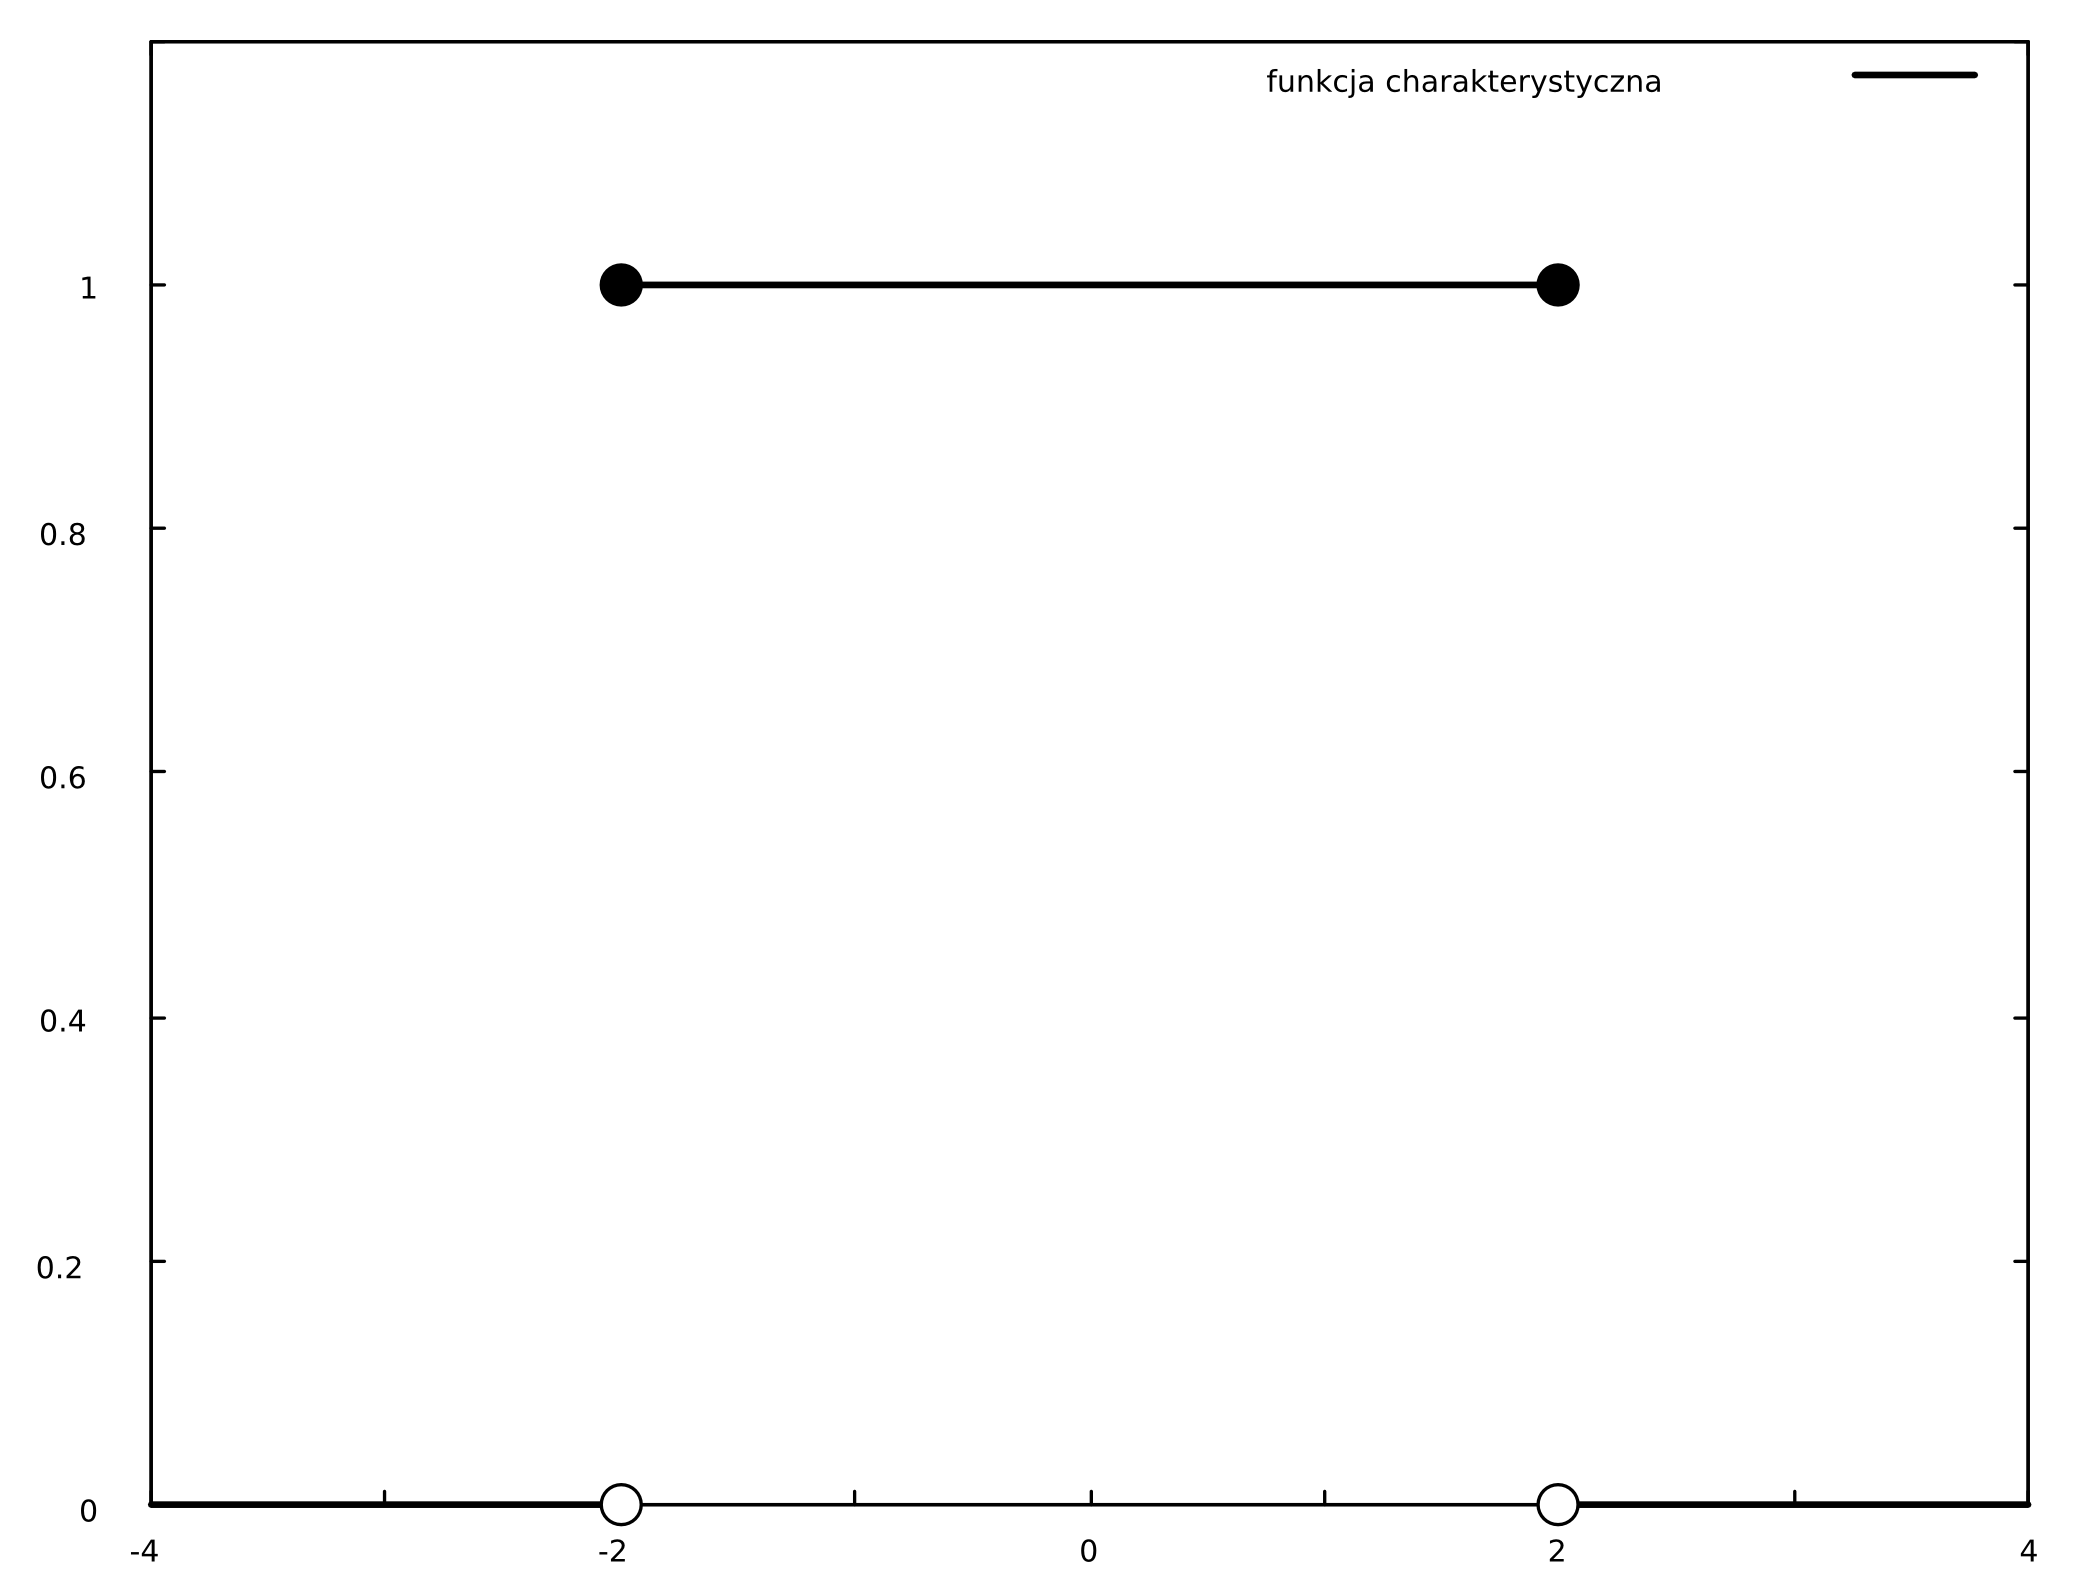
\includegraphics[width=\linewidth]
  	{chapters/fuzzylogic/funkcja_charakterystyczna}
  \caption{Funkcja charakterystyczna dla zbioru $x \in \mathcal{R} : -2 \leq x
  \leq 2 $}
  \label{fig:funkcja_charakterystyczna}
\end{figure}

Powyższa definicja mówi o tym, że jakiś element należy do zbioru lub nie. Jednak
czy w ,,realnym życiu'' zawsze możliwe jest jednoznaczne określenie, że coś
podoba się w $100\%$ lub nie? Albo czy coś jest zawsze w $100\%$ prawdą? W życiu
codziennym na pytanie ,,Czy to miejsce Ci się podoba?'', prócz odpowiedzi
,,tak'' i ,,nie'', bardzo często można usłyszeć: nie do końca, może być, nie
bardzo, jest super, zdecydowanie nie. Każda z tych odpowiedzi opisuje stopień
podobania się. Można się dowiedzieć na przykład, że pytanej osobie dane miejsce
się nie podoba, ale jest skłonna tam pójść.

Pomimo tego, że człowiek doskonale radzi sobie z odpowiedziami typu: ,,bardzo'',
,,około'', ,,mało'', ,,mniej więcej'', itp. to próba ich wyrażenia za pomocą
tradycyjnych zbiorów skazana jest na porażkę. Obserwacja ta była podstawą dla
Zadeha wprowadzenia pojęcia zbioru nieostrego (rozmytego) \cite{zadeh1965fuzzy}.

\begin{definition}[Zbiór rozmyty]
Jeżeli $\mathcal{X}$ jest kolekcją obiektów to zbiór rozmyty $A$ w przestrzeni
$\mathcal{X}$ określa się jako zbiór (klasyczny) par uporządkowanych
\begin{equation}
A = \{ (x, \mu_A(x)) : x \in \mathcal{X} \},
\end{equation}
gdzie $\mu_A$ jest funkcją przynależności zbioru rozmytego $A$ oraz $\mu_A(x)
\in [0,1]$ nazywany jest stopniem przynależności elementu $x$ do zbioru
rozmytego $A$. Tak zdefiniowany zbiór rozmyty jest tożsamy z funkcją
przynależności, gdyż ta zgodnie z teorią mnogości określona jest jako zbiór par
uporządkowanych.
\end{definition}

Przykładową funkcję przynależności opisującą sformułowanie ,,około zera'' można
zaprezentować jak na rysunku \ref{fig:funkcja_przynaleznosci}.

\begin{figure}[ht]
  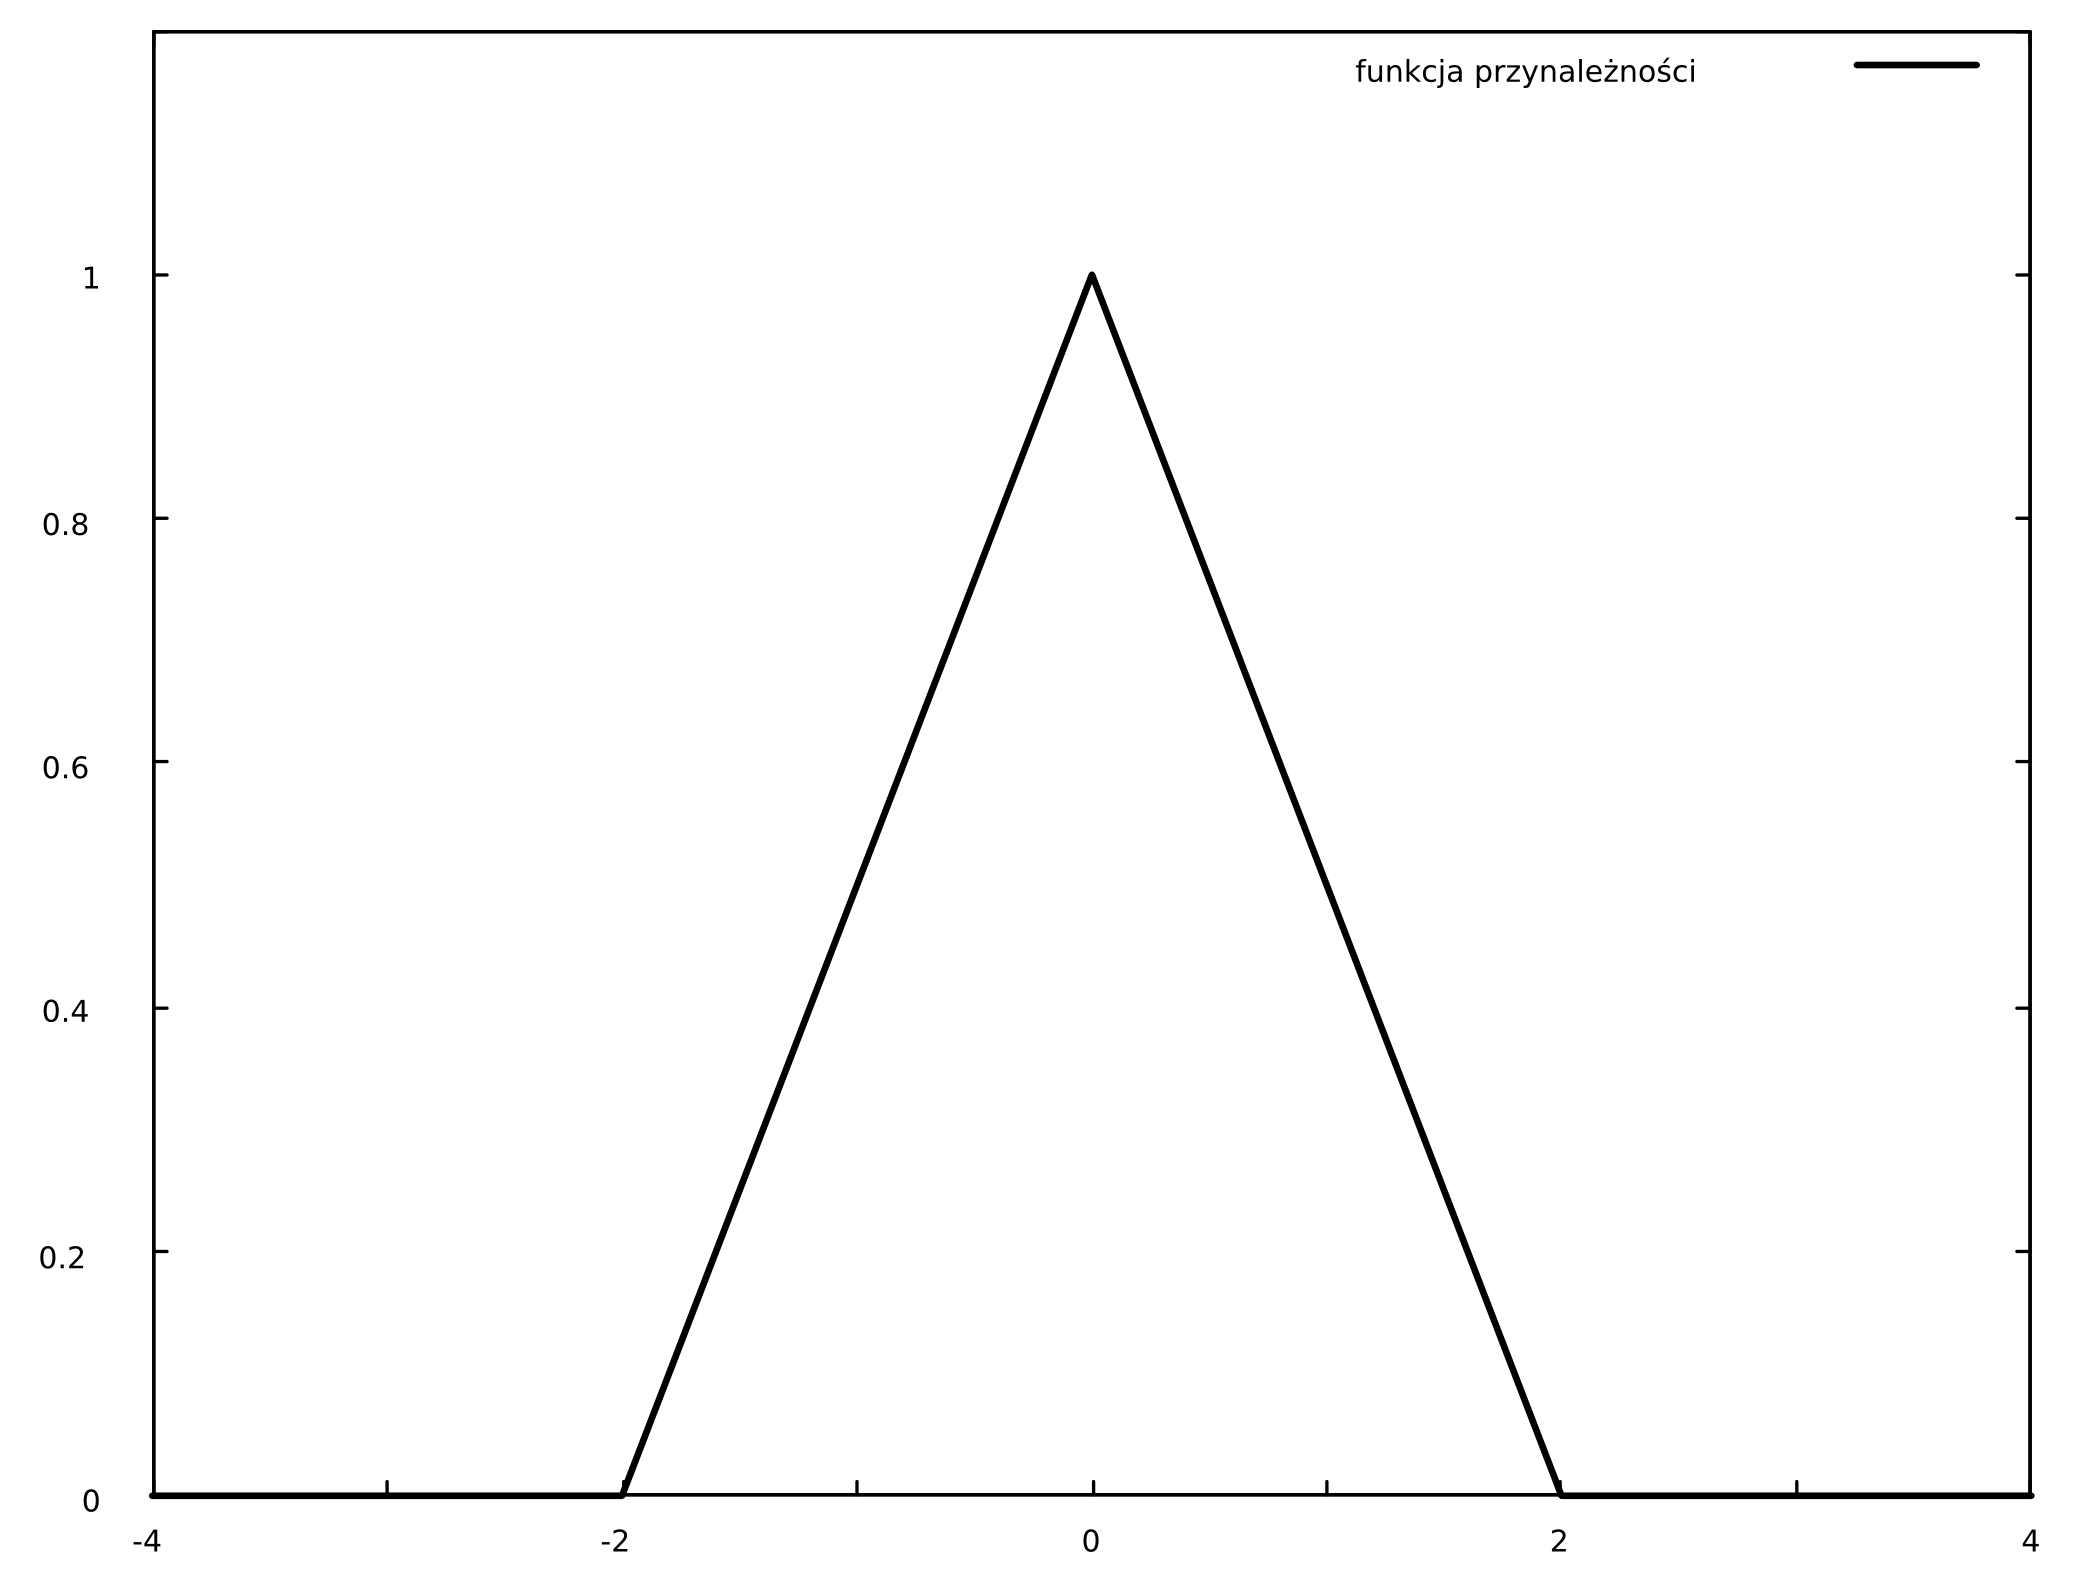
\includegraphics[width=\linewidth]
  	{chapters/fuzzylogic/funkcja_przynaleznosci}
  \caption{Przykładowa funkcja przynależności}
  \label{fig:funkcja_przynaleznosci}
\end{figure}

Ze zbiorami rozmytymi wiąże się kilka przydatnych pojęć przedstawionych poniżej.

\begin{definition}[Nośnik zbioru] Niech $A : X \rightarrow [0,1].$ Zbiór:
\begin{equation}
  \mathrm{supp}(A) = \{ x \in \mathcal{X} : A(x) > 0 \}.
\end{equation}
nazywamy \emph{nośnikiem} (ang. \textit{support}) zbioru nieostrego.
Nośnik zbioru to inaczej zbiór tych elementów $x$, które mają znaczenie dla $A$.  
\end{definition}

\begin{definition}
Niech $A : X \rightarrow [0,1]$.
\begin{itemize}
  \item \emph{t-przekrojem} i \emph{jądrem} $A$ nazywa się odpowiednio zbiory
  \newline $A_t = \{ x \in X : A(x) \geq t \}$ i $ker(A) = A_1$.
  \item Mówimy, że $A$ jest \emph{skończony}, gdy $supp(A)$ jest zbiorem
  skończonym, a w przeciwnym przypadku $A$ nazywamy \emph{nieskończonym} zbiorem
  nieostrym.
  \item Jeżeli $ker(A) \neq \emptyset,$ mówimy, że $A$ jest \emph{normalny}, a w
  przeciwnym przypadku $A$ nazywamy \emph{podnormalnym} lub \emph{subnormalnym}.
  \item Jeśli $|supp(A)| = 1$, $A$ nazywamy \emph{singletonem}.
\end{itemize}
\end{definition}

\emph{Normalny} zbiór rozmyty nakłada ograniczenie na funkcję przynależności,
które z punktu widzenia teorii jest nieistotne, jednakże w zastosowaniach
praktycznych okazuje się bardzo przydatne. Jeżeli zbiór rozmyty $A$ jest
normalny to wartość funkcji przynależności można interpretować jako procent na
ile dany element $x$ należy do $A$.

Jednym z ważniejszych pojęć zbiorów rozmytych wykorzystywanym przy modelowaniu
podejmowania decyzji jest \emph{zmienna lingwistyczna}. Rozważmy zdania:
\begin{itemize}
  \item[] \emph{Tamto drzewo jest wysokie.}
  \item[] \emph{Ta książka jest droga.}
\end{itemize}

W pierwszym zdaniu atrybutem drzewa jest jego wysokość. Atrybut ten przyjmuje
wartość ,,wysokie''. W drugim przykładzie atrybutem książki jest cena, której
wartość to ,,droga''. Sposób pojmowania tych wartości lingwistycznych może być
różny dla różnych osób, dlatego każda taka wartość charakteryzowana jest zbiorem
rozmytym.

\begin{definition} Zmienną lingwistyczną nazywamy czwórkę $(N,X,T,M_N)$, gdzie

\begin{tabular}{ll}
  $N$ & \qquad nazwa zmiennej (np. \textit{wiek}), \\
  $X$ & \qquad przestrzeń rozważań (np. [0, 125] lat), \\
  $T$ & \qquad zbiór wartości lingwistycznych (terminów) (np. \{młody, średni,
  stary\}), \\
  $M_N$ & \qquad funkcja semantyczna $M_N : T \rightarrow \textrm{zbiór funkcji
  przynależności}$.
\end{tabular}
\end{definition}

Na rysunku \ref{fig:zmienna_lingwistyczna} pokazane są przykładowe funkcje
przynależności dla zbioru termów \{mróz, zimno, chłodno, ciepło, gorąco\}
zmiennej lingwistycznej o nazwie ,,temperatura''. W tym przypadku przestrzenią
rozważań są stopnie Celsjusza od $-25$ do $45$ stopni.

\begin{figure}[ht]
  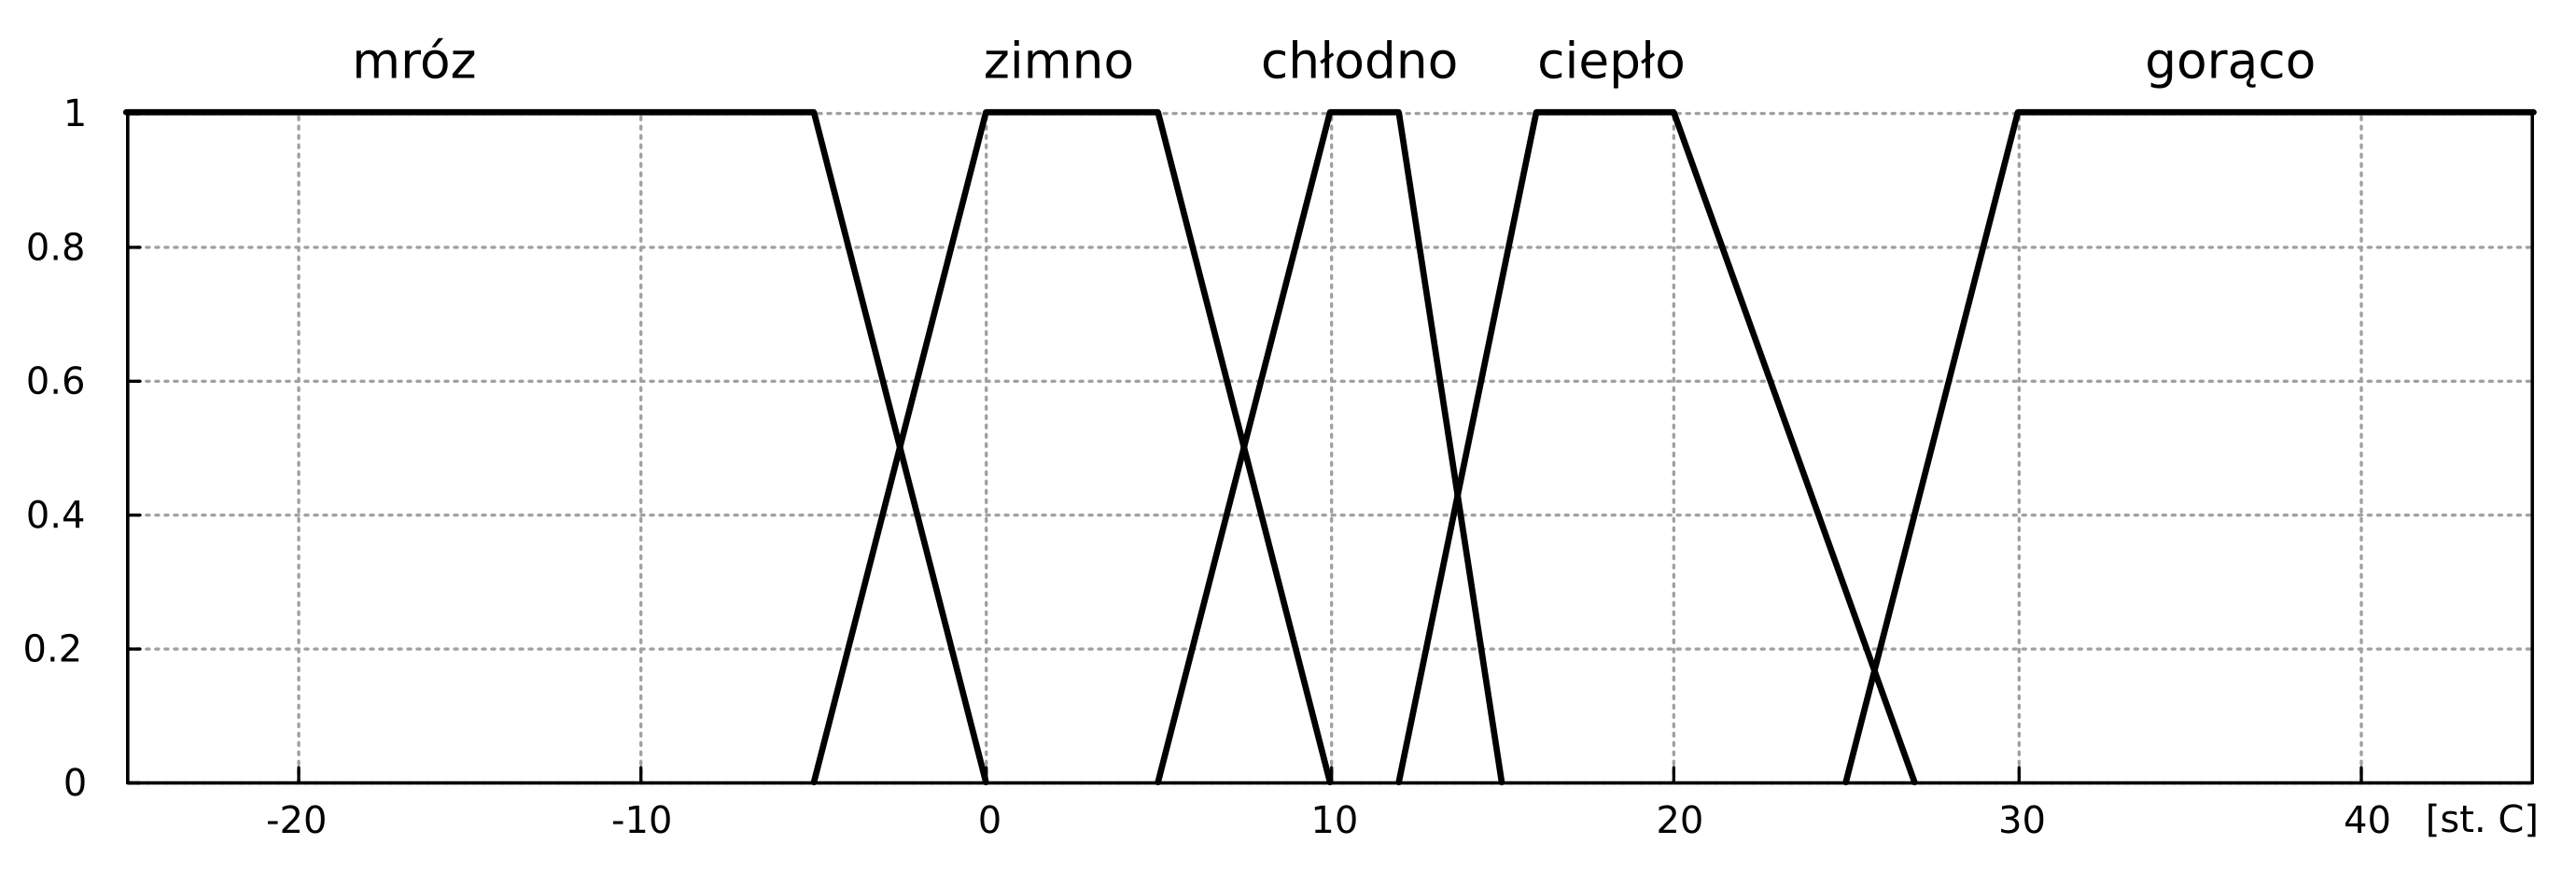
\includegraphics[width=\linewidth]
  	{chapters/fuzzylogic/zmienna_lingwistyczna}
  \caption{Funkcje przynależności dla zmienne lingwistycznej ,,temperatura''}
  \label{fig:zmienna_lingwistyczna}
\end{figure}

\subsection{Operacje na zbiorach rozmytych}
W klasycznej teorii mnogości podstawowe operacje na zbiorach to: dopełnienie,
suma, iloczyn. Nie inaczej jest w przypadku zbiorów rozmytych, ale wszystkie te
operacje można zdefiniować na wiele sposobów.

W swojej pierwszej publikacji, Zadeh \cite{zadeh1965fuzzy} zdefiniował
podstawowe operacje, generalizujące operacje dla zbiorów ostrych, w następujący
sposób:

\begin{definition}
Dopełnienie zbioru rozmytego $A$ określa się jako zbiór rozmyty, którego funkcja
przynależności dana jest w następujący sposób:
\begin{equation}
\mu_{\neg A}(x) = 1 - \mu_A(x).
\end{equation}
\end{definition}

\begin{definition}
Suma dwóch zbiorów rozmytych $A$ i $B$ określa się jako zbiór rozmyty, którego
funkcja przynależności dana jest w następujący sposób:
\begin{equation}
\mu_{A \cup B}(x) = \max(\mu_A(x), \mu_B(x)).
\end{equation}
\end{definition}

\begin{definition}
Iloczyn dwóch zbiorów rozmytych $A$ i $B$ określa się jako zbiór rozmyty,
którego funkcja przynależności dana jest w następujący sposób:
\begin{equation}
\mu_{A \cap B}(x) = \min(\mu_A(x), \mu_B(x)).
\end{equation}
\end{definition}

Powyższe definicje sumy i przekroju, mimo swej powszechności i intuicyjności,
nie są jedynym sposobem zdefiniowania tych operacji. Rozróżnia się dwie rodziny
funkcji, które dzięki spełnienie pewnych warunków, mogą zastąpić operację
maksimum i minimum w definicjach, odpowiednio, sumy i przekroju zbiorów
rozmytych.

\begin{definition}[t-norma]
Funkcję $t : [0,1] \times [0,1] \rightarrow [0,1]$ nazywamy \emph{normą
triangularną} (krótko: \emph{t-normą}) jeżeli:
\begin{itemize}
  \item funkcja $t$ jest monotoniczna $$a \leq b \Rightarrow t(a,c) \leq
  t(b,c),$$
  \item funkcja $t$ spełnia warunek przemienności $$t(a,b) = t(b,a),$$
  \item funkcja $t$ spełnia warunek łączności $$t(a, t(b,c)) = t(t(a,b),c),$$
  \item funkcja $t$ spełnia warunek brzegowy $$t(a,1)=a,$$
\end{itemize}
gdzie $a, b, c \in [0,1]$.
\end{definition}

Najczęściej spotykane t-normy to:
\begin{itemize}
  \item minimum $$t(a,b) = \min(a,b),$$
  \item iloczyn algebraiczny $$t(a,b) = a \cdot b,$$
  \item t-norma Łukasiewicza $$t(a,b) = \max(0, a+b-1).$$
\end{itemize}

\begin{definition}[t-konorma]
Funkcję $s : [0,1] \times [0,1] \rightarrow [0,1]$ nazywamy \emph{konormą
triangularną} (krótko: \emph{t-konormą}) jeżeli:
\begin{itemize}
  \item funkcja $s$ jest monotoniczna $$a \leq b \Rightarrow s(a,c) \leq
  s(b,c),$$
  \item funkcja $s$ spełnia warunek przemienności $$s(a,b) = s(b,a),$$
  \item funkcja $s$ spełnia warunek łączności $$s(a, s(b,c)) = s(s(a,b),s),$$
  \item funkcja $s$ spełnia warunek brzegowy $$s(a,0)=a,$$
\end{itemize}
gdzie $a, b, c \in [0,1]$.
\end{definition}

Najczęściej spotykane t-konormy to:
\begin{itemize}
  \item maksimum $$s(a,b) = \max(a,b),$$
  \item suma probabilistyczna $$s(a,b) = a+b-ab,$$
  \item t-konorma Łukasiewicza $$s(a,b) = \min(a+b,1).$$
\end{itemize}

Ogólne przecięcie i sumę zbiorów rozmytych definiuje się jako:
$$\mu_{A \cap B}(x) = t(\mu_A(x), \mu_B(x)), $$
$$\mu_{A \cup B}(x) = s(\mu_A(x), \mu_B(x)). $$

Przedstawione operacje na zbiorach rozmytych mają własności przemienności,
łączności i rozdzielności, zachodzą również prawa de Morgana. Jest to przydatne
w zastosowaniach praktycznych, jednak w ogólności:

$$A \cap \bar{A} \neq \emptyset \textrm{ i } A \cup \bar{A} \neq \mathcal{X}.$$

\subsection{Relacja rozmyta}
Relacje rozmyte pozwalają sformalizować nieprecyzyjne sformułowania typu ,,$x$
jest prawie równe $y$'' lub ,,$x$ jest znacznie większe od $y$''.

\begin{definition}[Relacja rozmyta]
Relację rozmytą $\mathcal{R}$ między dwoma niepustymi zbiorami ostrymi $X$ i $Y$
nazywamy zbiór rozmyty określony na iloczynie kartezjańskim $X \times Y$, tzn.
$$\mathcal{R} \subseteq X \times Y = \{ (x,y) : x \in X, y \in Y \}.$$
Innymi słowy relacja rozmyta jest zbiorem par
\begin{equation}
\mathcal{R} = \{ ((x,y), \mu_{\mathcal{R}}(x,y)) : x \in X, y \in Y \},
\end{equation}
gdzie $\mu_{\mathcal{R}} : X \times Y \rightarrow [0,1]$ jest funkcją
przynależności. Funkcja ta każdej parze $(x,y)$ przypisuje jej stopień
przynależności $\mu_{\mathcal{R}}(x,y)$, który ma interpretację siły powiązania
między elementami $x$ i $y$.
\end{definition}

\begin{example}
Dana są przestrzenie rozważań $X=\{ x_1,x_2,x_3 \} = \{3,4,5\}$,
$Y=\{y_1,y_2,y_3\} = \{4,5,6\}$ oraz relacja $\mathcal{R} \subseteq X \times Y$
interpretowana jako ,,$y$ jest mniej więcej równe $x$''. Niech relację
$\mathcal{R}$ reprezentuje macierz $[a_{ij}]$, gdzie wartość $a_{ij}$ oznacza
stopień powiązania między elementami $x_i$ i $y_j$:
$$A = 
\begin{pmatrix}
0.8 & 0.6 & 0.4 \\
  1 & 0.8 & 0.6 \\
0.8 &   1 & 0.8
\end{pmatrix}.
$$
Równoważnie można zapisać:
$$
A = 
\left\{ 
	\begin{array}{cl}
	  1, & \quad \textrm{jeżeli } x = y, \\
      0.8, & \quad \textrm{jeżeli } |x - y| = 1, \\
      0.6, & \quad \textrm{jeżeli } |x - y| = 2, \\
      0.4, & \quad \textrm{jeżeli } |x - y| = 3. \\
  	\end{array} 
  \right.
$$
\end{example}

\subsection{Operatory agregacji}
Wiadomo już jak sumować zbiory rozmyte, jak tworzyć ich przecięcie oraz jak
definiuje się relacje. Z punktu widzenia poniższej pracy niezwykle przydatna
jest możliwość agregacji danych. Mając zebrane dane o preferencjach ekspertów w
postaci zbiorów rozmytych, należy zebrać je w jedność w celu zbadania poziomu
konsensusu.

\begin{definition}
\emph{Operatorem agregacji} nazywamy odwzorowanie
$$
Agr: \cup_{n \geq 1} [0,1]^n \rightarrow [0,1],
$$
spełniające następujące warunki:
\begin{itemize}
  \item monotoniczność $Agr(a_1, a_2, \dotsc, a_n) \leq Agr(b_1, b_2, \dotsc,
  b_n), \text{ gdy } a_i \leq b_i \text{ dla } i=1,2,\dotsc,n$,
  \item warunek identyczności $Agr(a) = a$ dla każdego $a \in [0,1]$,
  \item warunki brzegowe $Agr(0, \dotsc, 0) = 0, Agr(1, \dotsc, 1) = 1$.
\end{itemize}
\end{definition}

Jednymi z najbardziej popularnych i najczęściej wykorzystywanych jest rodzina
operatorów uporządkowanej średniej ważonej OWA (ang. \textit{Ordered Weighted
Averaging}).

\begin{definition}
Operator OWA wymiaru $n$ jest to odwzorowanie $U : [0,1]^n \rightarrow [0,1]$
z przypisanym wektorem wag $w=(w_1,w_2,\dotsc,w_n)^T$ take, że
\begin{equation}
F(a_1,a_2,\dotsc,a_n) = w_1b_1 + w_2b_2 + \dotsb + w_nb_n,
\end{equation}
gdzie $w_i \in [0,1]$ dla $i=1,\dotsc, n$ oraz $\sum_{i=1}^{n} w_i = 1$, a ciąg
$(b_i)_{i=1,n}$ powstaje przez nierosnące uporządkowanie wyrazów ciągu
$(a_i)_{i=1,n}$
\end{definition}

Operator OWA zapewnia ciągłe przejście z ,,bezwzględnego i'' do ,,bezwzględnego
lub'' poprzez korygowanie wektora wag $w$. Wektor wag $w$ może być ustalony przy
użyciu funkcji kwantyfikatora $Q(x)$ w następujący sposób:
$$w_i = Q(\frac{i}{n}) - Q(i - \frac{1}{n}).$$

Kwantyfikator $Q$ może być reprezentowany jako zbiór rozmyty taki, że dla
każdego $x \in [0,1]$, $Q(x)$ oznacza stopień, w jakim $x$ obiektów spełnia
pojęcie symbolizowane przez $Q$. Zatem stopień dominacji grupy, w której
,,większość'' ekspertów popiera alternatywę $a$ może być określony jako:
$$e(a) = F_Q(e^1(a),e^2(a),\dotsc,e^m(a)),$$
gdzie $F_Q$ jest operatorem OWA. Wektor wag $w_Q = (w_1,w_2,\dotsc,w_m)$ może
być ustalony przy pomocy następującej funkcji kwantyfikatora $Q$:
$$
Q(x) = 
\left\{ 
	\begin{array}{cl}
	  1	,				& \quad  x > b, \\
      \frac{x-a}{b-a}, 	& \quad  a \leq x \leq b \;\; a,b \in [0,1], \\
      0 ,				& \quad  x < a. \\
  	\end{array} 
  \right.
$$

Rysunki \ref{fig:kwantyfikator_lingwistyczny_wiekszosc} oraz
\ref{fig:kwantyfikator_lingwistyczny_polowa} przedstawiają dwa przykładowe typy
kwantyfikatorów, odpowiednio ,,Większość'' oraz ,,Co najmniej połowa''.

\begin{figure}[ht]
  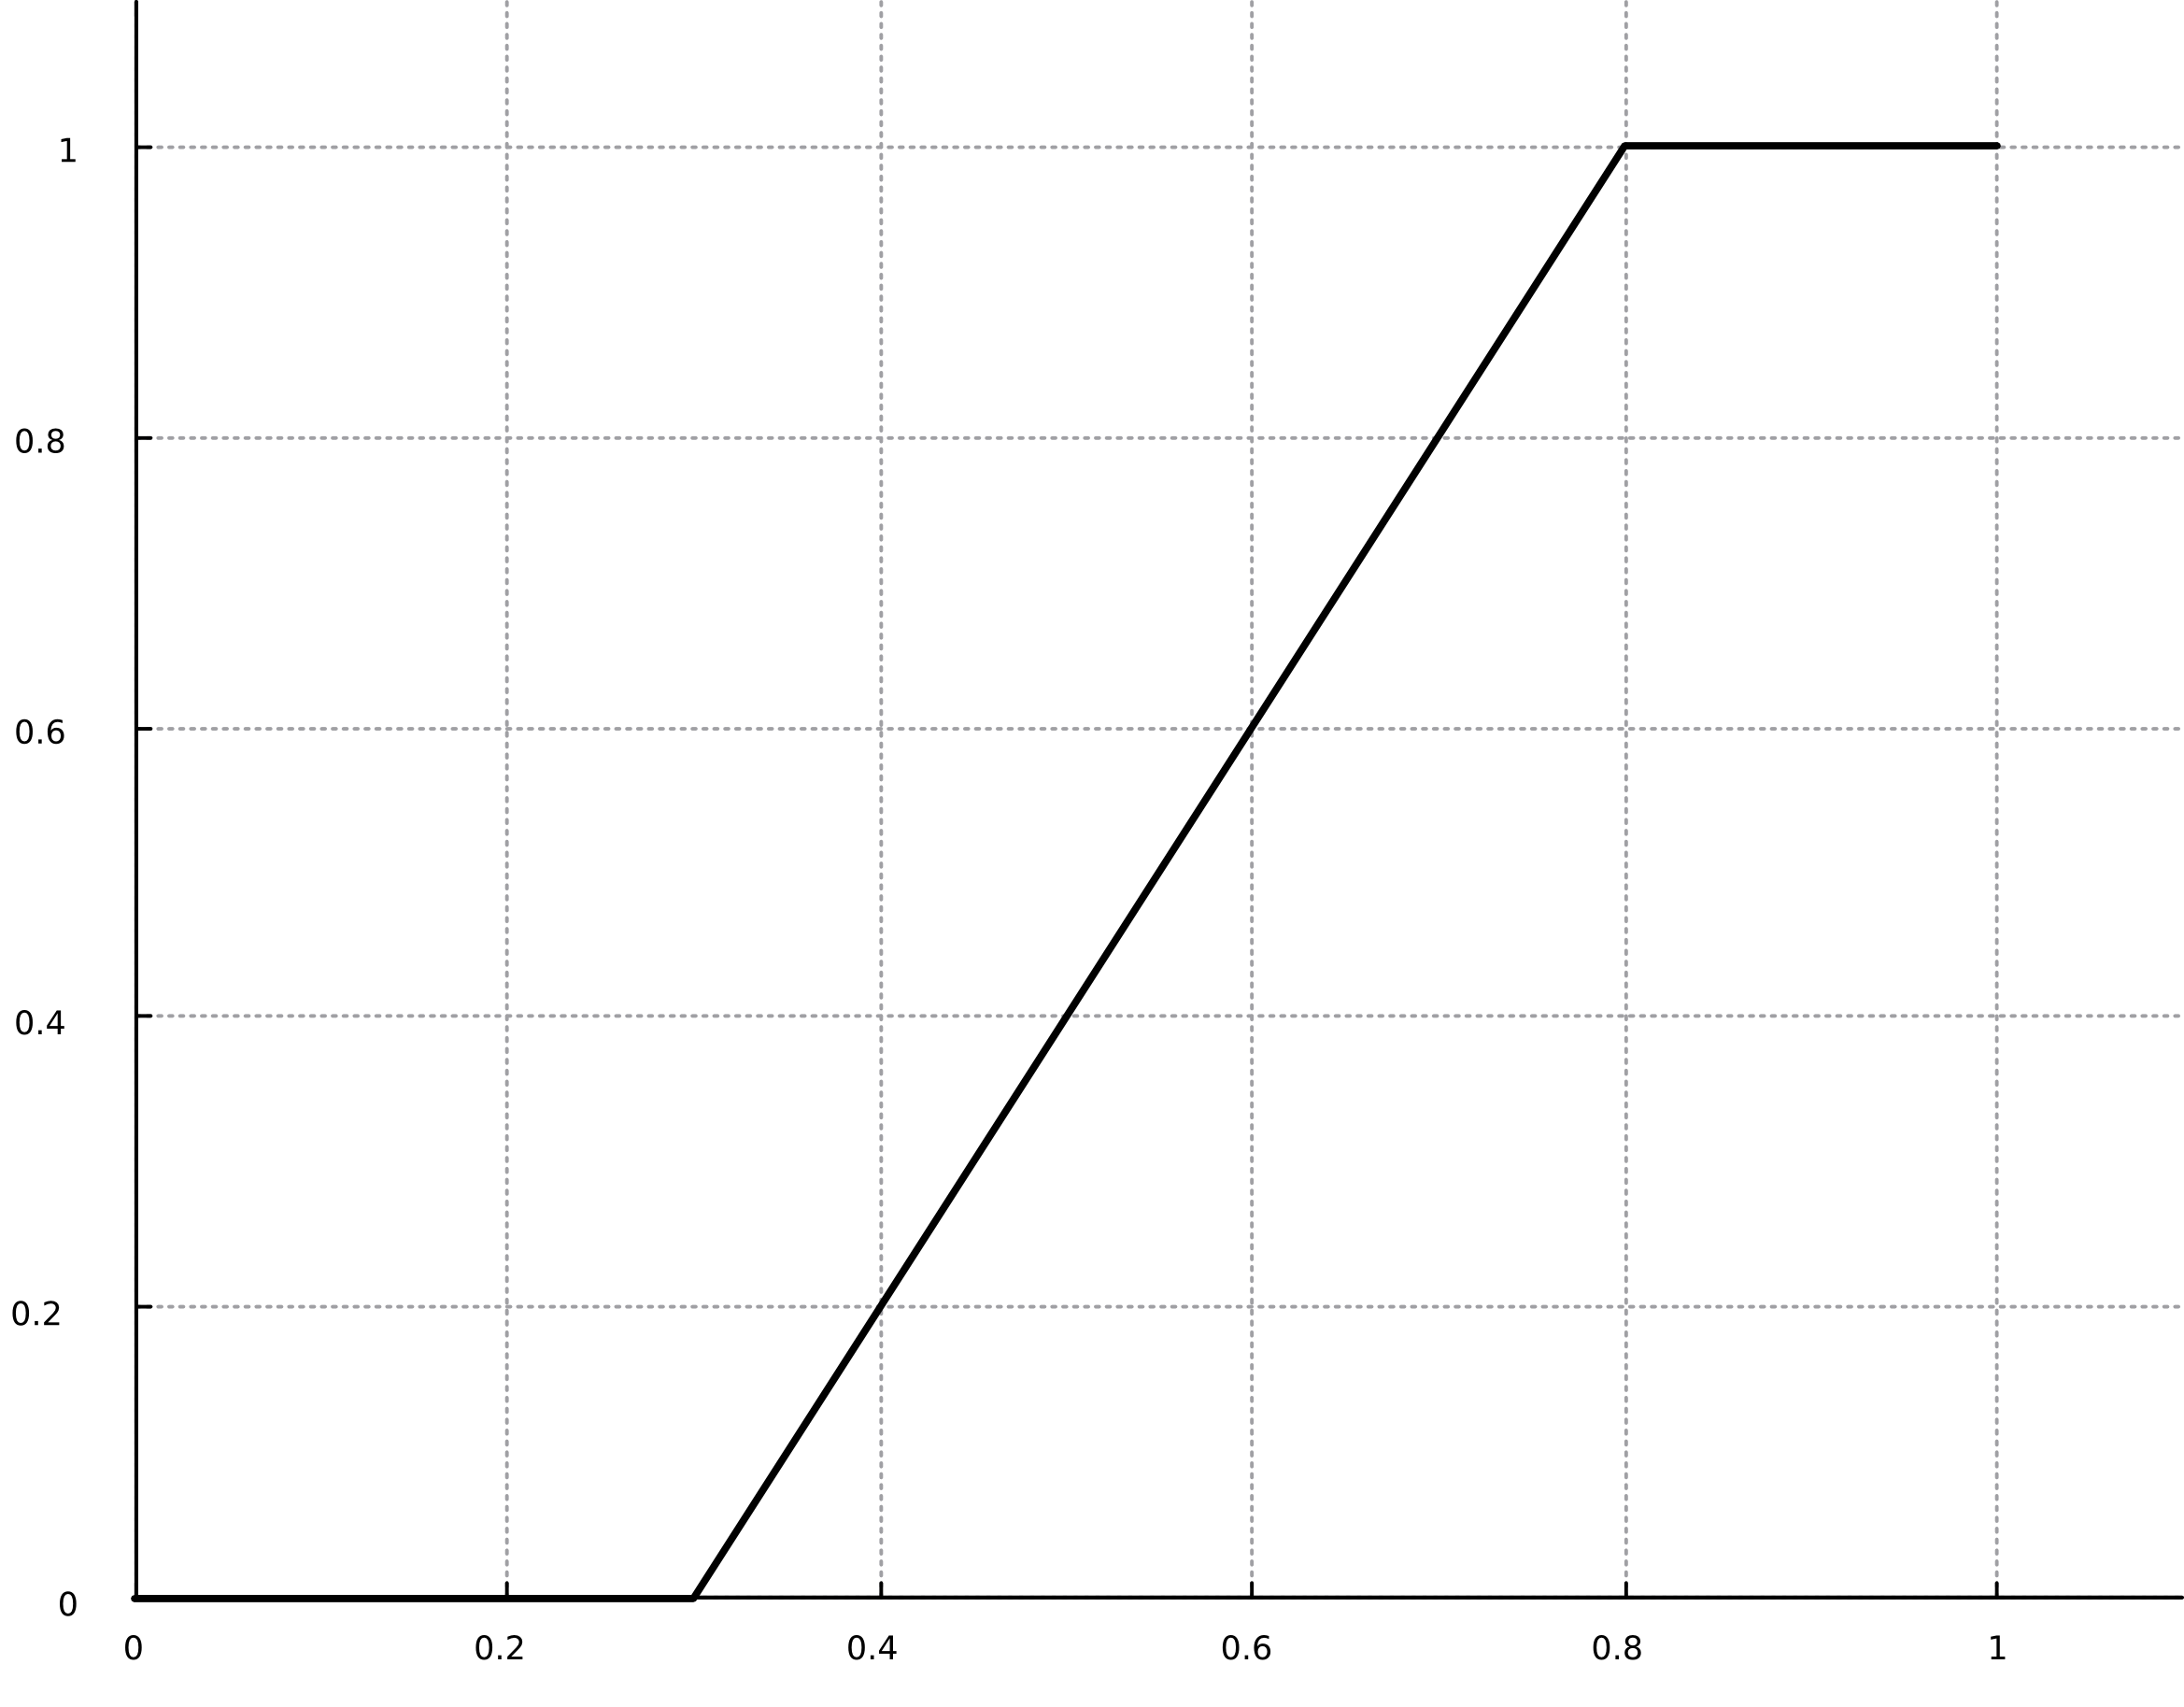
\includegraphics[width=\linewidth]
  	{chapters/fuzzylogic/fuzzy_most}
  \caption{Kwantyfikator lingwistyczny ,,Większość''}
  \label{fig:kwantyfikator_lingwistyczny_wiekszosc}
\end{figure}

\begin{figure}[ht]
  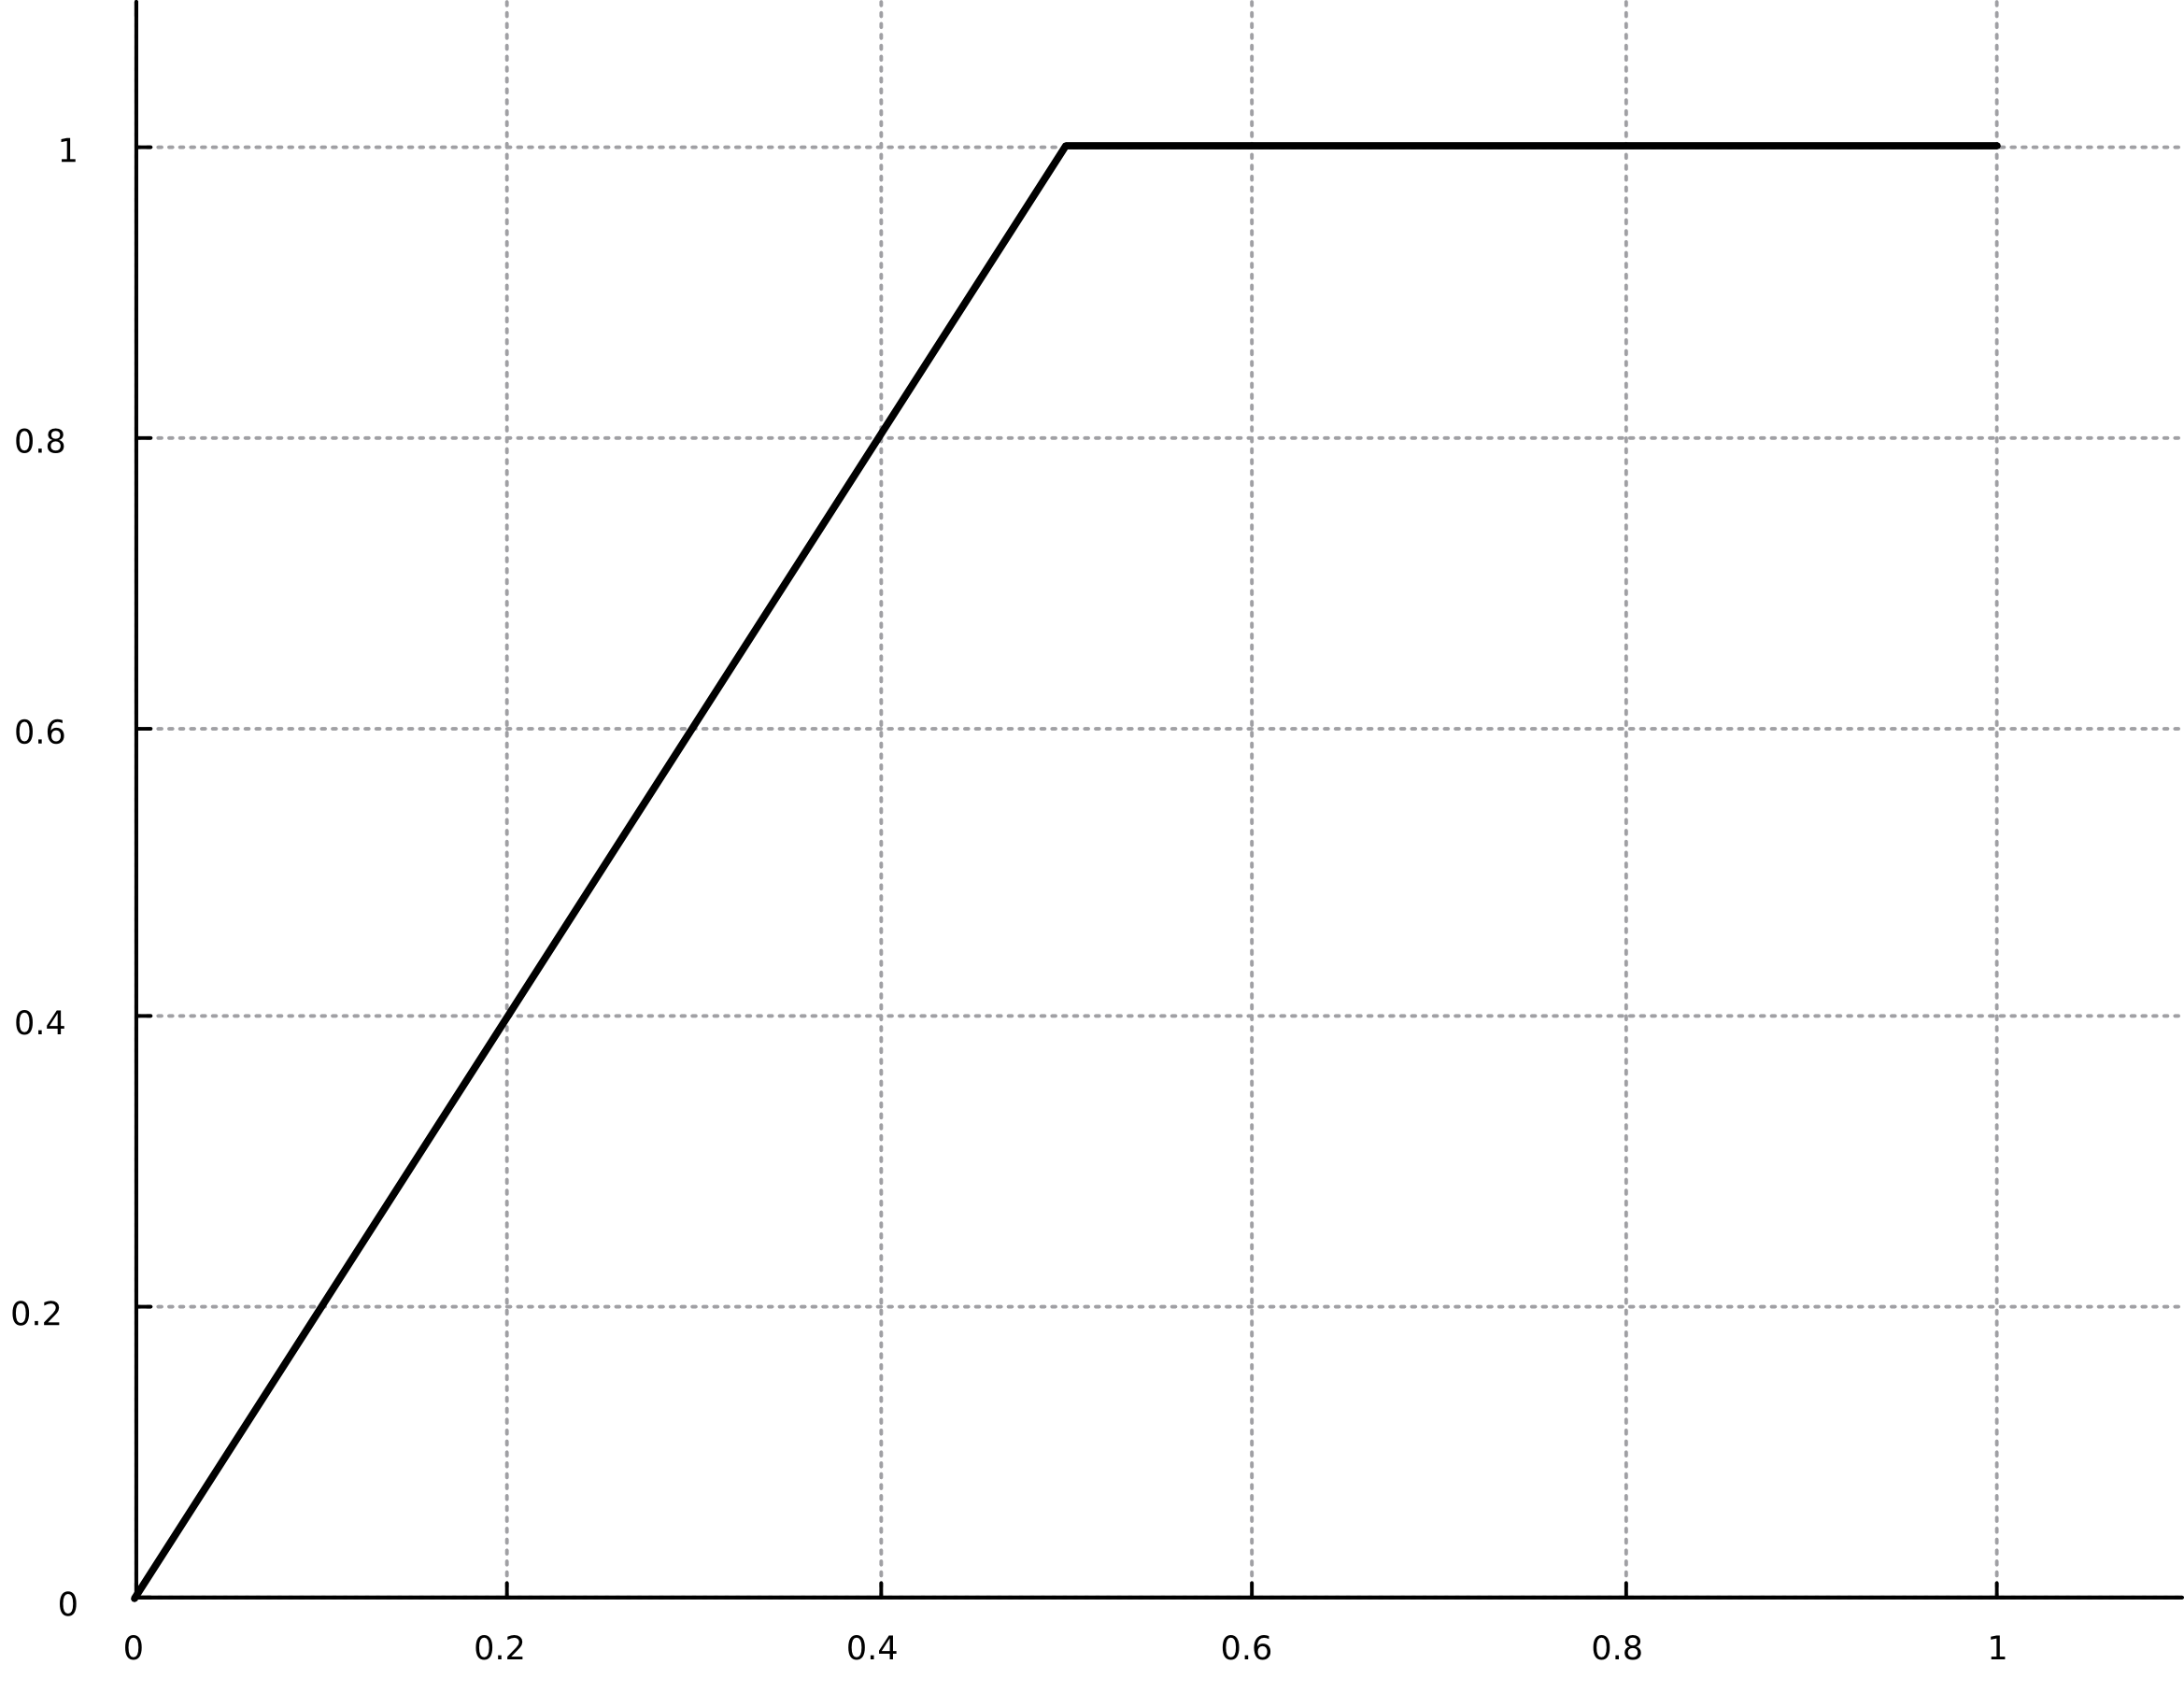
\includegraphics[width=\linewidth]
  	{chapters/fuzzylogic/fuzzy_half}
  \caption{Kwantyfikator lingwistyczny ,,Co najmniej połowa''}
  \label{fig:kwantyfikator_lingwistyczny_polowa}
\end{figure}

\begin{example}
Załóżmy, że stopnie preferencji każdego z ekspertów dla alternatywy $a$
wyglądają następująco: $[0.58, 0.33, 0.92, 0.08, 0.72, 0.65]$, a do agregacji
został użyty kwantyfikator lingwistyczny $Q = \textrm{,,większość''}$. Stopień
dominacji grupowej wynosi:
$$e(a) = F_{Q_{Most}}(0.58, 0.33, 0.92, 0.08, 0.72, 0.65) = 0.613,$$
gdzie $w=(0, 0.07, 0.33, 0.60, 0, 0).$
\end{example}

Z powyższego przykładu wynika, że kwantyfikator lingwistyczny ,,Większość''
bierze środkową część uporządkowanych ocen ekspertów i oblicza ich sumę ważoną.
Z powodzeniem można skorzystać z innych kwantyfikatorów, odpowiednio do
sytuacji. Ponadto przy pomocy operatora OWA można modelować sytuację, w której
decydenci zamierzają oceniać tak, że ,,większość'' kryteriów jest spełniona.

\section{Zastosowanie logiki rozmytej w podejmowaniu decyzji}
Podejmowanie decyzji to proces analizy zaistniałej sytuacji, z której istnieją 
co najmniej dwie drogi dalszego postępowania. Proces ten można oprzeć na 
racjonalnym działaniu, czyli logicznym myśleniu i chłodnej kalkulacji. Niestety 
w życiu codziennym wiele decyzji podejmowanych jest z wykorzystaniem własnych 
odczuć, emocji, intuicji. Zatem podejmowanie decyzji to proces nie tylko 
racjonalny i nowoczesne systemy wspomagania decyzji wprowadzają mechanizmy 
pozwalające na ocenę intuicyjną oraz działaniu na niepewnych i niepełnych 
danych.

Człowiek z natury porusza się w środowisku nieprecyzyjnym. Każdy potrafi 
powiedzieć, czy w danej restauracji smakuje mu jedzenie (wyśmienite, smaczne,
przeciętne, niesmaczne, $\dotsc$). Jednak mało kto potrafi w sposób ścisły, z
użyciem liczb, sprecyzować swoją opinię. Jest to subiektywna sprawa, osobiste
odczucie. Nieprecyzyjność jest całkowicie naturalna i stanowi nieodłączny
element podejmowania decyzji.

Grupowe podejmowanie decyzji jest bardzo dobrym przykładem na to, że 
modelowanie tego procesu tylko przy użyciu metod precyzyjnych jest zadaniem 
bardzo trudnym, a co więcej - nienaturalnym.

Poniższy podrozdział prezentuje przykłady wykorzystania logiki rozmytej w 
modelowaniu poszczególnych etapów grupowego podejmowania decyzji.

\subsection{Reprezentacja preferencji}
Każdy z decydentów powinien wyrazić swoją opinię na temat dostępnych alternatyw 
w sposób wygodny i naturalny, możliwie jak najbardziej zbliżony do naturalnego. 
Większość ludzi zapytanych o porównanie dwóch rozwiązań, jako pierwsze powie, 
że rozwiązanie pierwsze woli bardziej niż drugie. Może też paść odpowiedź ,,dużo
bardziej'', ,,zdecydowanie'' i tym podobne. Tego typu przypadki bardzo dobrze
modeluje powszechnie stosowana tak zwana rozmyta relacja preferencji.

Żeby w pełni wykorzystać możliwości rozmytej relacji preferencji, wykorzystuje 
się zmienną lingwistyczną. To dzięki niej możliwe jest wykorzystanie w 
obliczeniach wyrażeń lingwistycznych takich jak ,,mniej'' i ,,bardziej''.

Rozmytym oraz tradycyjnym metodom wydobywania i reprezentacji preferencji 
decydentów poświęcony został osobny rozdział.

\subsection{Ocena globalna}
Zazwyczaj na początku wszyscy członkowie grupy posiadają odmienne zdanie na 
temat wyboru rozwiązania. Proces osiągania konsensusu jest niezbędny w każdym 
procesie grupowego podejmowania decyzji. Tradycyjnie konsensus jest postrzegany 
jako pełna zgoda wszystkich decydentów. Oczywiście, ten typ konsensusu jest 
idealny i bardzo trudny do osiągnięcia. Z tego względu, jest to proces 
dynamiczny i iteracyjny. W jakiś sposób należy sprawdzać, czy odpowiedni poziom 
zgody został osiągnięty. Realizuje się to poprzez obliczenie globalnej oceny 
alternatyw i porównanie jej z indywidualnymi.

We wcześniejszym podpunkcie zostały przedstawione zbiory rozmyte jako doskonałe
narzędzie do reprezentacji ocen poszczególnych decydentów. Jest to również
doskonałe narzędzie do agregacji tych ocen w jedną zbiorczą ocenę. W tym celu
wykorzystuje się operatory agregacji, szczególnie operator OWA. Dzięki niemu
można mówić o konsensusie ,,większości'' albo ,,więcej niż $70\%$''
grupy.

\subsection{Tworzenie rankingu}
Po fazie agregacji następuje faza eksploatacji uzyskanych danych, czyli moment,
w którym ocena globalna alternatyw zamieniana jest na globalny ranking. Globalny
ranking uzyskuje się poprzez użycie dwóch stopni wyboru alternatyw:
kwantyfikator stopnia dominacji QGDD (ang. \textit{quantifier guided dominance
degree}) oraz kwantyfikator stopnia nie-dominacji QGNDD (ang.
\textit{quantifier guided non dominance degree}). Pierwszy z nich jest używany,
aby uzyskać przewagę jaką posiada dana alternatywa nad pozostałymi w kontekście rozmytej większości. Drugi
kwantyfikator natomiast, podaje stopień w jakim każda z alternatyw nie jest
zdominowana przez rozmytą większość zbioru alternatyw. Sposób w jaki należy
połączyć te dwie informacje w celu uzyskania rankingu jest opisany w kolejnych
rozdziałach.

	
	\chapter{Sposoby reprezentacji preferencji}
	Odkrycie preferencji użytkownika ma na celu poznanie opinii na temat różnych 
usług i przedmiotów. Są one kluczem w wielu aplikacjach, takich jak systemy 
rekomendacji, filtrowanie lub wyszukiwanie informacji. W przypadku podejmowania 
decyzji poznanie preferencji jest jednym z podstawowych elementów systemu. Aby 
osiągnąć konsensus i przedstawić propozycje rozwiązań problemu, trzeba poznać 
zdanie decydentów na temat każdej z alternatyw. Okazuje się, że nie jest to 
łatwe zadanie, ponieważ każdy z ekspertów posiada swoje własne idee, cele, 
motywacje i osobowość. Prowadzi to do wniosku, że różne osoby mogą wyrażać 
swoje preferencje na różne sposoby.

W tym rozdziale zostanie przedstawiony ogólny model poznawania preferencji. 
Następnie wprowadzone zostaną klasyczne sposoby reprezentacji. Warto zwrócić 
uwagę na to, że przed metodami klasycznymi stoi kilka wyzwań. Jednym z nich 
jest niepewność. Na przykład opis alternatywy lub wprowadzone preferencje mogą 
być niepełne i nieprecyzyjne ze względu na brak pełnej informacji, niewiedzę 
lub niezdecydowanie osoby. Dlatego na koniec rozdziału omówione zostaną metody 
wykorzystujące zbiory rozmyte.


\section{Model ogólny}
Scenariusz idealny zakłada poproszenie użytkowników o wyrażenie swoich 
preferencji na temat różnych cech ocenianego problemu. W praktyce ma to jednak 
ograniczone zastosowanie, a także nie zawsze jest to możliwe. Obiecującym 
źródłem odkrywania preferencji mogą być komentarze użytkowników. Ogólny schemat 
odkrywania i przetwarzania preferencji przedstawiony jest na rysunku
\ref{fig:ogolny_model_preferencji}.

Schemat zaproponowany przez Zenebe et al. [8] składa się z czterech głównych 
elementów: wydobycie i prezentacja cech, odkrycie preferencji, reprezentacja 
preferencji, zastosowanie wydobytych informacji.

\begin{figure}[ht]
  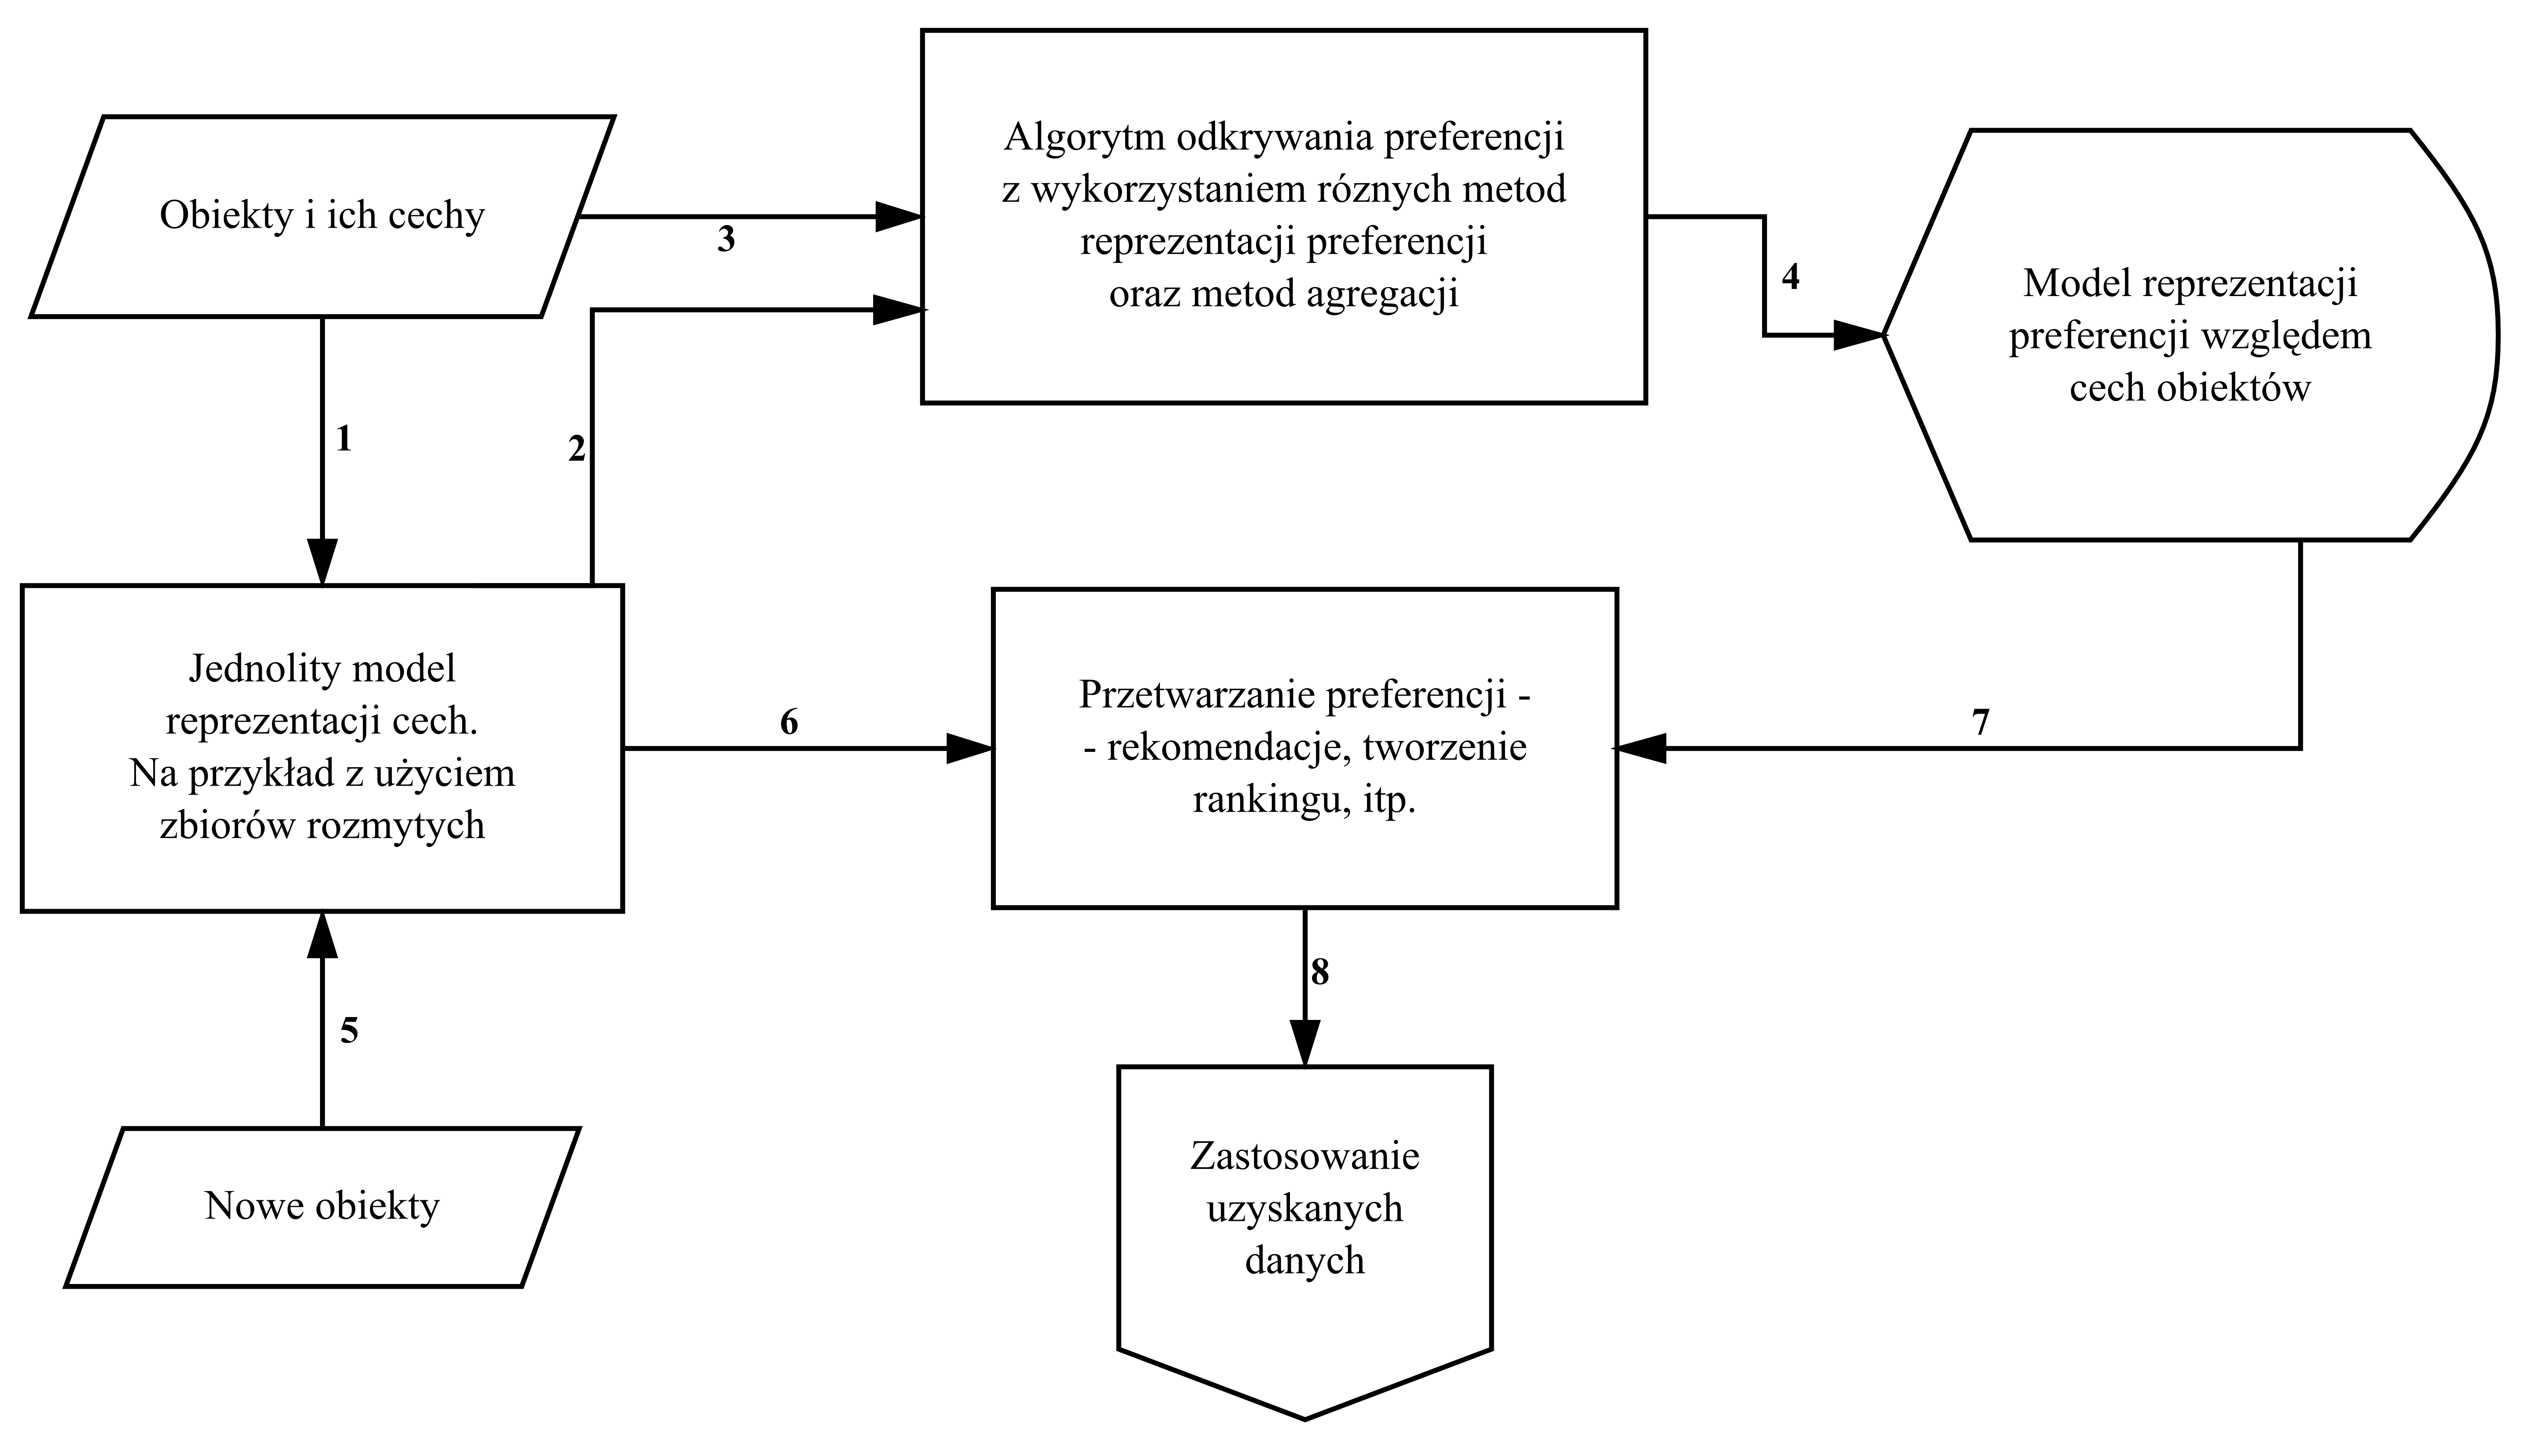
\includegraphics[width=\linewidth]
  	{chapters/preferences/ogolny_model_preferencji}
  \caption{Schemat odkrywania i przetwarzania preferencji}
  \label{fig:ogolny_model_preferencji}
\end{figure}

\section{Metody klasyczne}

\subsection{Uporządkowanie alternatyw}

W tym przypadku, alternatywy uporządkowane są od najlepszej do najgorszej bez
żadnej dodatkowej informacji. Formalnie, ekspert $e_k$ podaje swoje preferencje
dla zbioru alternatyw $\mathcal{X}$ jako indywidualne uporządkowanie alternatyw
$ O^k =$ $\{o^k(1), \dotsc,$ $o^k(n)\}$, gdzie $o^k(\cdot)$ jest funkcją
permutacji nad zbiorem indeksów $\{1,\dotsc,n\}$. Jak wspomniano wyżej, wynikiem
jest uporządkowany zbiór alternatyw.

\subsection{Multiplikatywna relacja preferencji}
W tym przypadku, preferencje ekspertów dla zbioru $\mathcal{X}$ opisane są przy
pomocy relacji preferencji $A^k \subset X \times X, A^k = a^k_{ij}$, gdzie
$a^k_{ij}$ wskazuje stopień intensywności preferencji alternatywy $x_i$ do
$x_j$. Innymi słowy, alternatywa $x_i$ jest $a^k_{ij}$ razy tak dobra jak $x_j$.

Nawiązując do pracy Millera \todo{bibl} nad postrzeganiem liczb, Saaty w swojej
pracy \todo{bibl} sugeruje używania w takich sytuacjach skali od $1$ do $9$.
Zatem $a^k_{ij} = 1$ interpretuje się jako obojętność lub brak różnicy dla
eksperta pomiędzy rozwiązaniami $x_i$ oraz $x_j$, $a^k_{ij}=9$ oznacza, że $x_i$
jest zdecydowanie bardziej preferowane niż $x_j$, natomiast $a^k_{ij} \in \{
2,3, \dotsc, 8\}$ oznacza oceny pośrednie. Z reguły zakłada się, że relacja jest
wzajemnie odwrotna, czyli $\forall_{i,j} \, a^k_{ij} \cdot a^k_{ji} = 1$.

\subsection{Funkcja użyteczności}
Użyteczność to inaczej zdolność dobra do zaspokajania potrzeb. Określa
subiektywną przyjemność, pożytek lub zadowolenie płynące z dokonanego wyboru.
Należy pamiętać, że użyteczność jest abstrakcją i ma charakter subiektywny,
podobnie jak pozostałe metody. Przy pomocy funkcji użyteczności, ekspert
przedstawia ocenę każdej z alternatyw zgodnie z użytecznością z jego punktu
widzenia. Formalnie, ekspert $e_k$ podaje swoje preferencje dla zbioru
alternatyw $\mathcal{X}$ jako zbiór $n$ wartości użyteczności $U^k = \{u^k_i;
i=1,\dotsc,n\}, u^k_i \in [0,1]$, gdzie $u^k_i$ reprezentuje wartość
użyteczności alternatywy $x_i$ daną przez eksperta $e_k$.

\section{Metody oparte na zbiorach rozmytych}
Teoria zbiorów rozmytych jest stosowana w grupowym podejmowaniu decyzji już od 
długiego czasu \todo{biblio}. Większość modeli opracowanych w literaturze jest 
opartych na rozmytej relacji preferencji, która może być uzyskana poprzez 
porównania pomiędzy parami różnych alternatyw przez ekspertów.

Z drugiej strony, wiele problemów dotyczy ilościowych aspektów, które mogą być 
ocenione przy użyciu konkretnych wartości liczbowych, czyli z użyciem opisanych 
wcześniej metod klasycznych. Jednakże, występuje bardzo dużo problemów o 
aspekcie jakościowym, które są bardzo trudne do oceny poprzez dokładne i ścisłe 
wartości. W takich przypadkach, podejście wykorzystujące zmienne lingwistyczne 
może być stosowane w celu uzyskania lepszego rozwiązania. Na przykład, gdy 
eksperci starają się ocenić komfort samochodu, gdzie są używane wyrażenia 
językowe, jak ,,dobry'', ,,niezły'', ,,słaby''.

\subsection{Rozmyta relacja preferencji}

\begin{definition}
Rozmyta relacja preferencji $R$ na zbiorze alternatyw $\mathcal{X}$ jest zbiorem
rozmytym na iloczynie kartezjańskim $X \times X$ z funkcją przynależności
$\mu_R : X \times X \rightarrow [0,1]$. Niech $P(x_i,x_j) \in R$ będzie rozmytą
relacją preferencji pomiędzy alternatywami $x_i$ i $x_j$. Wtedy $P(x_i,x_j)$
oraz $P(x_j,x_i)$ są zwrotne, tzn. $P(x_i,x_j) + P(x_j,x_i) = 1.$
\end{definition}

Niech $\mathcal{X}$ będzie zbiorem alternatyw oraz $x_i,x_j \in \mathcal{X}$.
Oznaczmy $P^k(x_i,x_j) = p^k_{ij}$, co oznacza stopień preferowania alternatywy 
$x_i$ nad $x_j$ względem kryterium $k$. Stąd $p^k_{ij} = 1$ oznacza, że
rozwiązanie $x_i$ jest bezwzględnie lepsze niż $x_j$, $p^k_{ij} \in (0.5; 1)$
przewagę $x_i$ nad $x_j$ (im większa wartość tym większa przewaga), a $x_j$,
$p^k_{ij} = 0.5$ brak różnicy pomiędzy rozwiązaniami.

Rozmyta relacja preferencji stosowana jest do modelowania
nieprecyzyjnej relacji pomiędzy różnymi rozwiązaniami. Aby zredukować uciążliwe
zadanie przypisywania stopni preferencji pomiędzy alternatywami przez ekspertów
($q(n-1)/2$ razy), rozmyta relacja preferencji między dwoma alternatywami $x_i$
i $x_j$ dla kryterium $k$ jest obliczana przez porównywanie parami ocen
lingwistycznych $g^t_k(x_i)$ i $g^t_k(x_j)$, które mogą być opisane jako liczby
rozmyte (szczegóły w następnym podpunkcie). W ten sposób, liczba ocen ekspertów
zmniejsza się do $qn$ razy.
\begin{figure}[ht]
  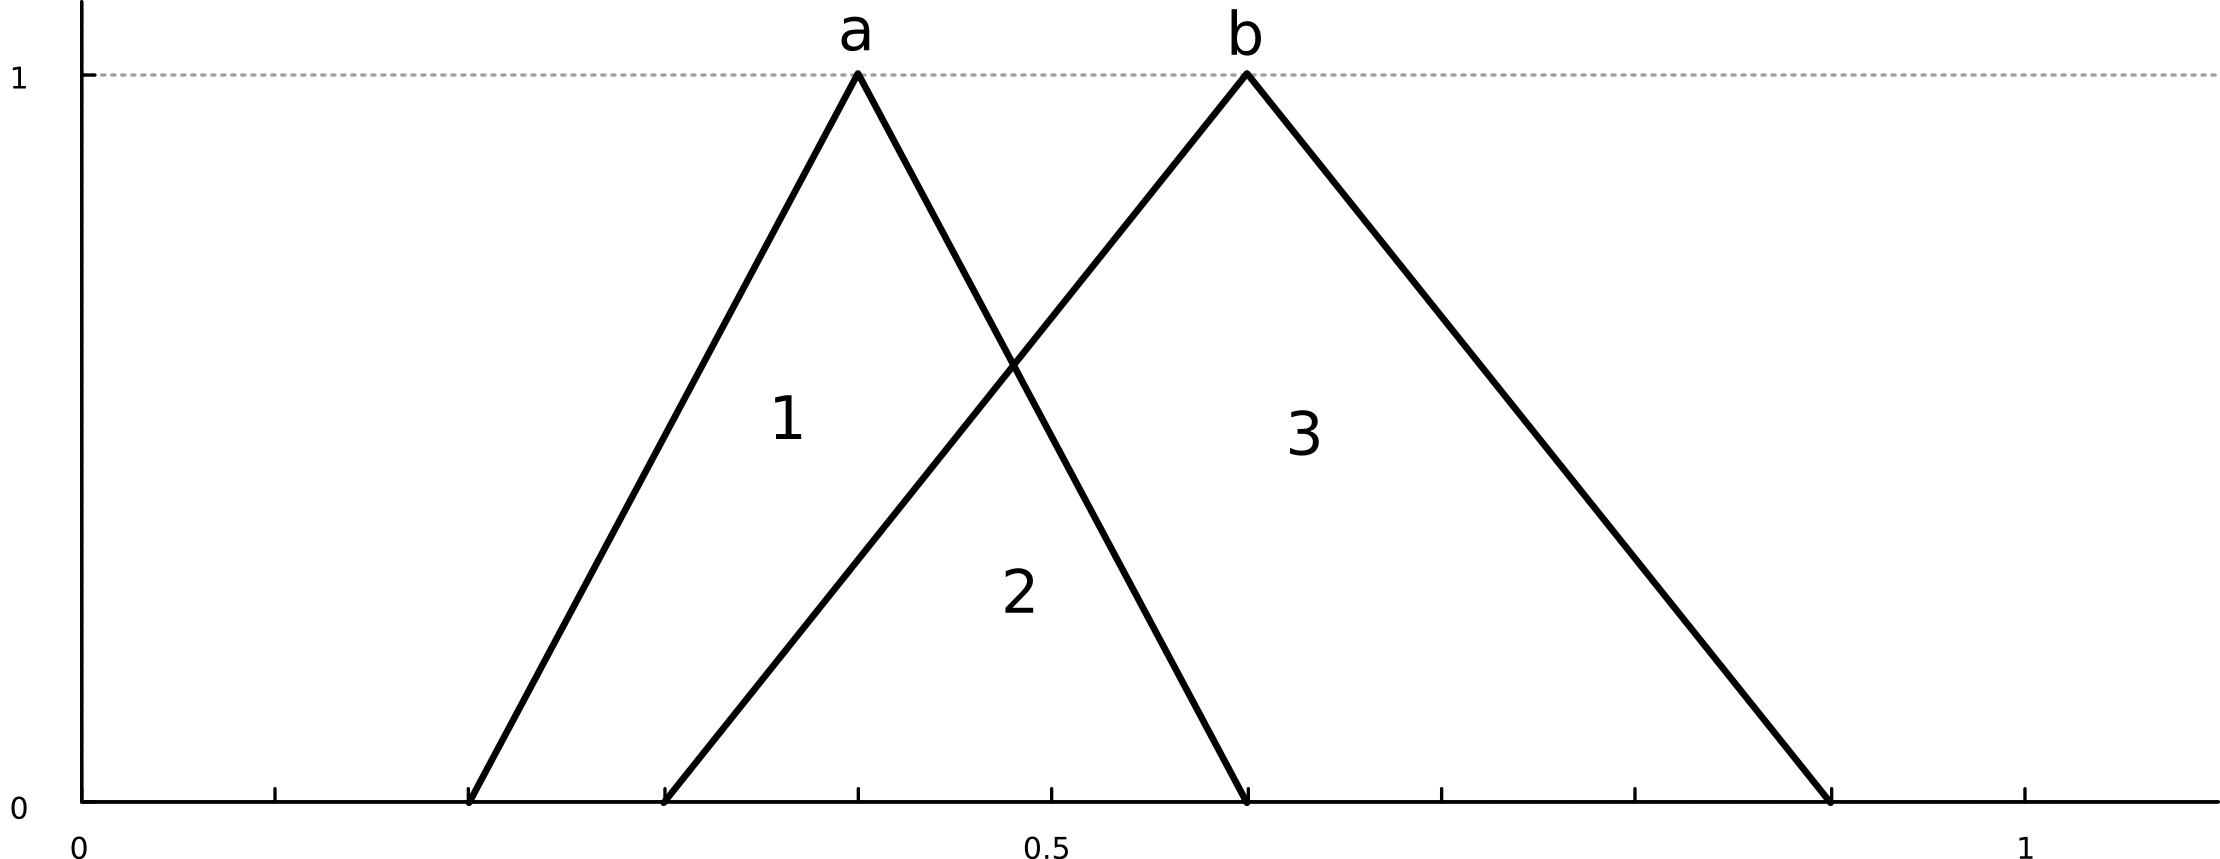
\includegraphics[width=\linewidth]
    {chapters/preferences/rozmyta_relacja_a}
  \caption{Przykład rozmytej relacji preferencji}
  \label{fig:rozmyta_relacja_preferencji}
\end{figure}
W literaturze istnieje wiele sposobów na zdefiniowanie relacji rozmytej pomiędzy
dwoma liczbami rozmytymi. W tej pracy zostanie użyte podejście Tsenga i Kleina
\todo{biblio} bazujące na odległości Hamminga ze względu na prostotę i
wydajność.

\begin{definition}
\label{def:rozmyta_relacja_preferencji}
Niech $a$ i $b$ będą liczbami rozmytymi. Rozmyte relacje preferencji $P(a,b)$ i
$P(b,a)$ zdefiniowane są w następujący sposób:
\begin{equation}
P(a,b) = \frac{D(a,b) + D(a \cap b, 0)}{D(a,0) + D(b,0)},
\end{equation}
\begin{equation}
P(b,a) = \frac{D(b,a) + D(a \cap b, 0)}{D(a,0) + D(b,0)},
\end{equation}
gdzie
\begin{itemize}
  \item[] $D(a,b)$ - powierzchnia, gdzie $a$ dominuje nad $b$,
  \item[] $D(b,a)$ - powierzchnia, gdzie $b$ dominuje nad $a$ (pole 1 i 3 na
  	rys. \ref{fig:rozmyta_relacja_preferencji}),
  \item[] $D(a,0)$ - powierzchnia $a$ (pole 1 i 2 na rys.
     \ref{fig:rozmyta_relacja_preferencji}),
  \item[] $D(b,0)$ - powierzchnia $b$ (pole 2 i 3 na rys.
  	\ref{fig:rozmyta_relacja_preferencji}),
  \item[] $D(a \cap b, 0)$ - przecięcie powierzchni $a$ i $b$ (pole 2 na rys.
  	\ref{fig:rozmyta_relacja_preferencji}).
\end{itemize}
\end{definition}

Dla przykładu rozmyta relacja preferencji na rysunku
\ref{fig:rozmyta_relacja_preferencji} jest liczona następująco:
$$P(a,b) = \frac{pole2}{(pole1 + pole2) + (pole2 + pole3)} = 0.18,$$
$$P(b,a) = \frac{(pole1 + pole3) + pole2}{(pole1 + pole2) + (pole2 + pole3)} =
0.82.$$

\subsection{Rozmyta relacja preferencji w przypadku wielu kryteriów}
Wyżej opisana rozmyta relacja preferencji pozwala ocenić alternatywy według
tylko jednego kryterium. W wielu przypadkach może się to okazać wystarczające,
ponieważ eksperci nie muszą oceniać poszczególnych cech rozwiązań, ale mogą
głosować bezpośrednio na nie po przeprowadzeniu dyskusji. Sytuacja komplikuje
się, kiedy każdy ekspert ocenia wyszczególnione wcześniej cechy rozwiązań (na
przykład cena, wygoda, wykonanie samochodu). W wyniku otrzymywany jest zbiór
relacji - po jednej na parę ekspert-kryterium. Aby uzyskać dane pozwalające na
uporządkowanie alternatyw należy połączyć wszystkie wyniki każdego eksperta
osobno.

Niech $p^t_k(x_i,x_j)$ będzie rozmytą relacją preferencji pomiędzy alternatywami
$x_i$ i $x_j$ dla kryterium $c_k$ oraz eksperta $e^t$ liczoną według definicji
\ref{def:rozmyta_relacja_preferencji}:
$$p^t_k(x_i,x_j) = P(g^t_k(x_i),g^t_k(x_j)).$$

Zbiorcza rozmyta relacja preferencji pomiędzy alternatywami $x_i$ i $x_j$ dla
eksperta $e^t$ może być uzyskana jako ważona suma wartości $p^t_k(x_i,x_j)$ po
wszystkich kryteriach $p^t(x_i,x_j) = \sum_{k=1}^{q} w_k \times p^t_k(x_i,x_j)$,
gdzie $\sum_{k=1}^{q} w_k = 1$.

Ostatecznie możliwe jest uporządkowanie alternatyw w częściowym porządku poprzez
wyliczenie stopnia dominacji każdej z alternatyw, czyli jak bardzo ekspert
$e^t$ wspiera dane rozwiązanie $x_i$. Oblicza się to jako średnia z
$p^t(x_i,x_j) \text{ dla } x_j \in \mathcal{X} \text{ i } x_j \neq x_i \colon
h^t(x_i) = \frac{1}{n-1} \sum_{x_j \in \mathcal{X}, x_j \neq x_i} p^t(x_i,x_j).$

\subsection{Ocena lingwistyczna}
Rozmyte podejście lingwistyczne używa zmiennych lingwistycznych, które
uczestniczą w procesie oceniania przy pomocy terminologii językowej zamiast
wartości liczbowych. Takie podejście jest odpowiednie dla wielu problemów,
ponieważ umożliwia przedstawienie indywidualnych preferencji w bardziej
bezpośredniej i odpowiedniej formie wtedy, gdy nie jest możliwe wyrażenie ich
precyzyjnie.

Zmienne lingwistyczne różnią się od numerycznych tym, że ich wartości nie są
liczbami, ale słowami lub zdaniami w naturalnym lub sztucznym języku. Ponieważ
słowa, generalnie, są mniej precyzyjne niż liczby, koncepcja zmiennych
lingwistycznych zapewnia środki umożliwiające zbliżoną charakteryzację zjawisk,
które są zbyt skomplikowane lub za słabo zdefiniowane, żeby opisać je w
tradycyjnych kategoriach ilościowych.
\begin{figure}[ht]
  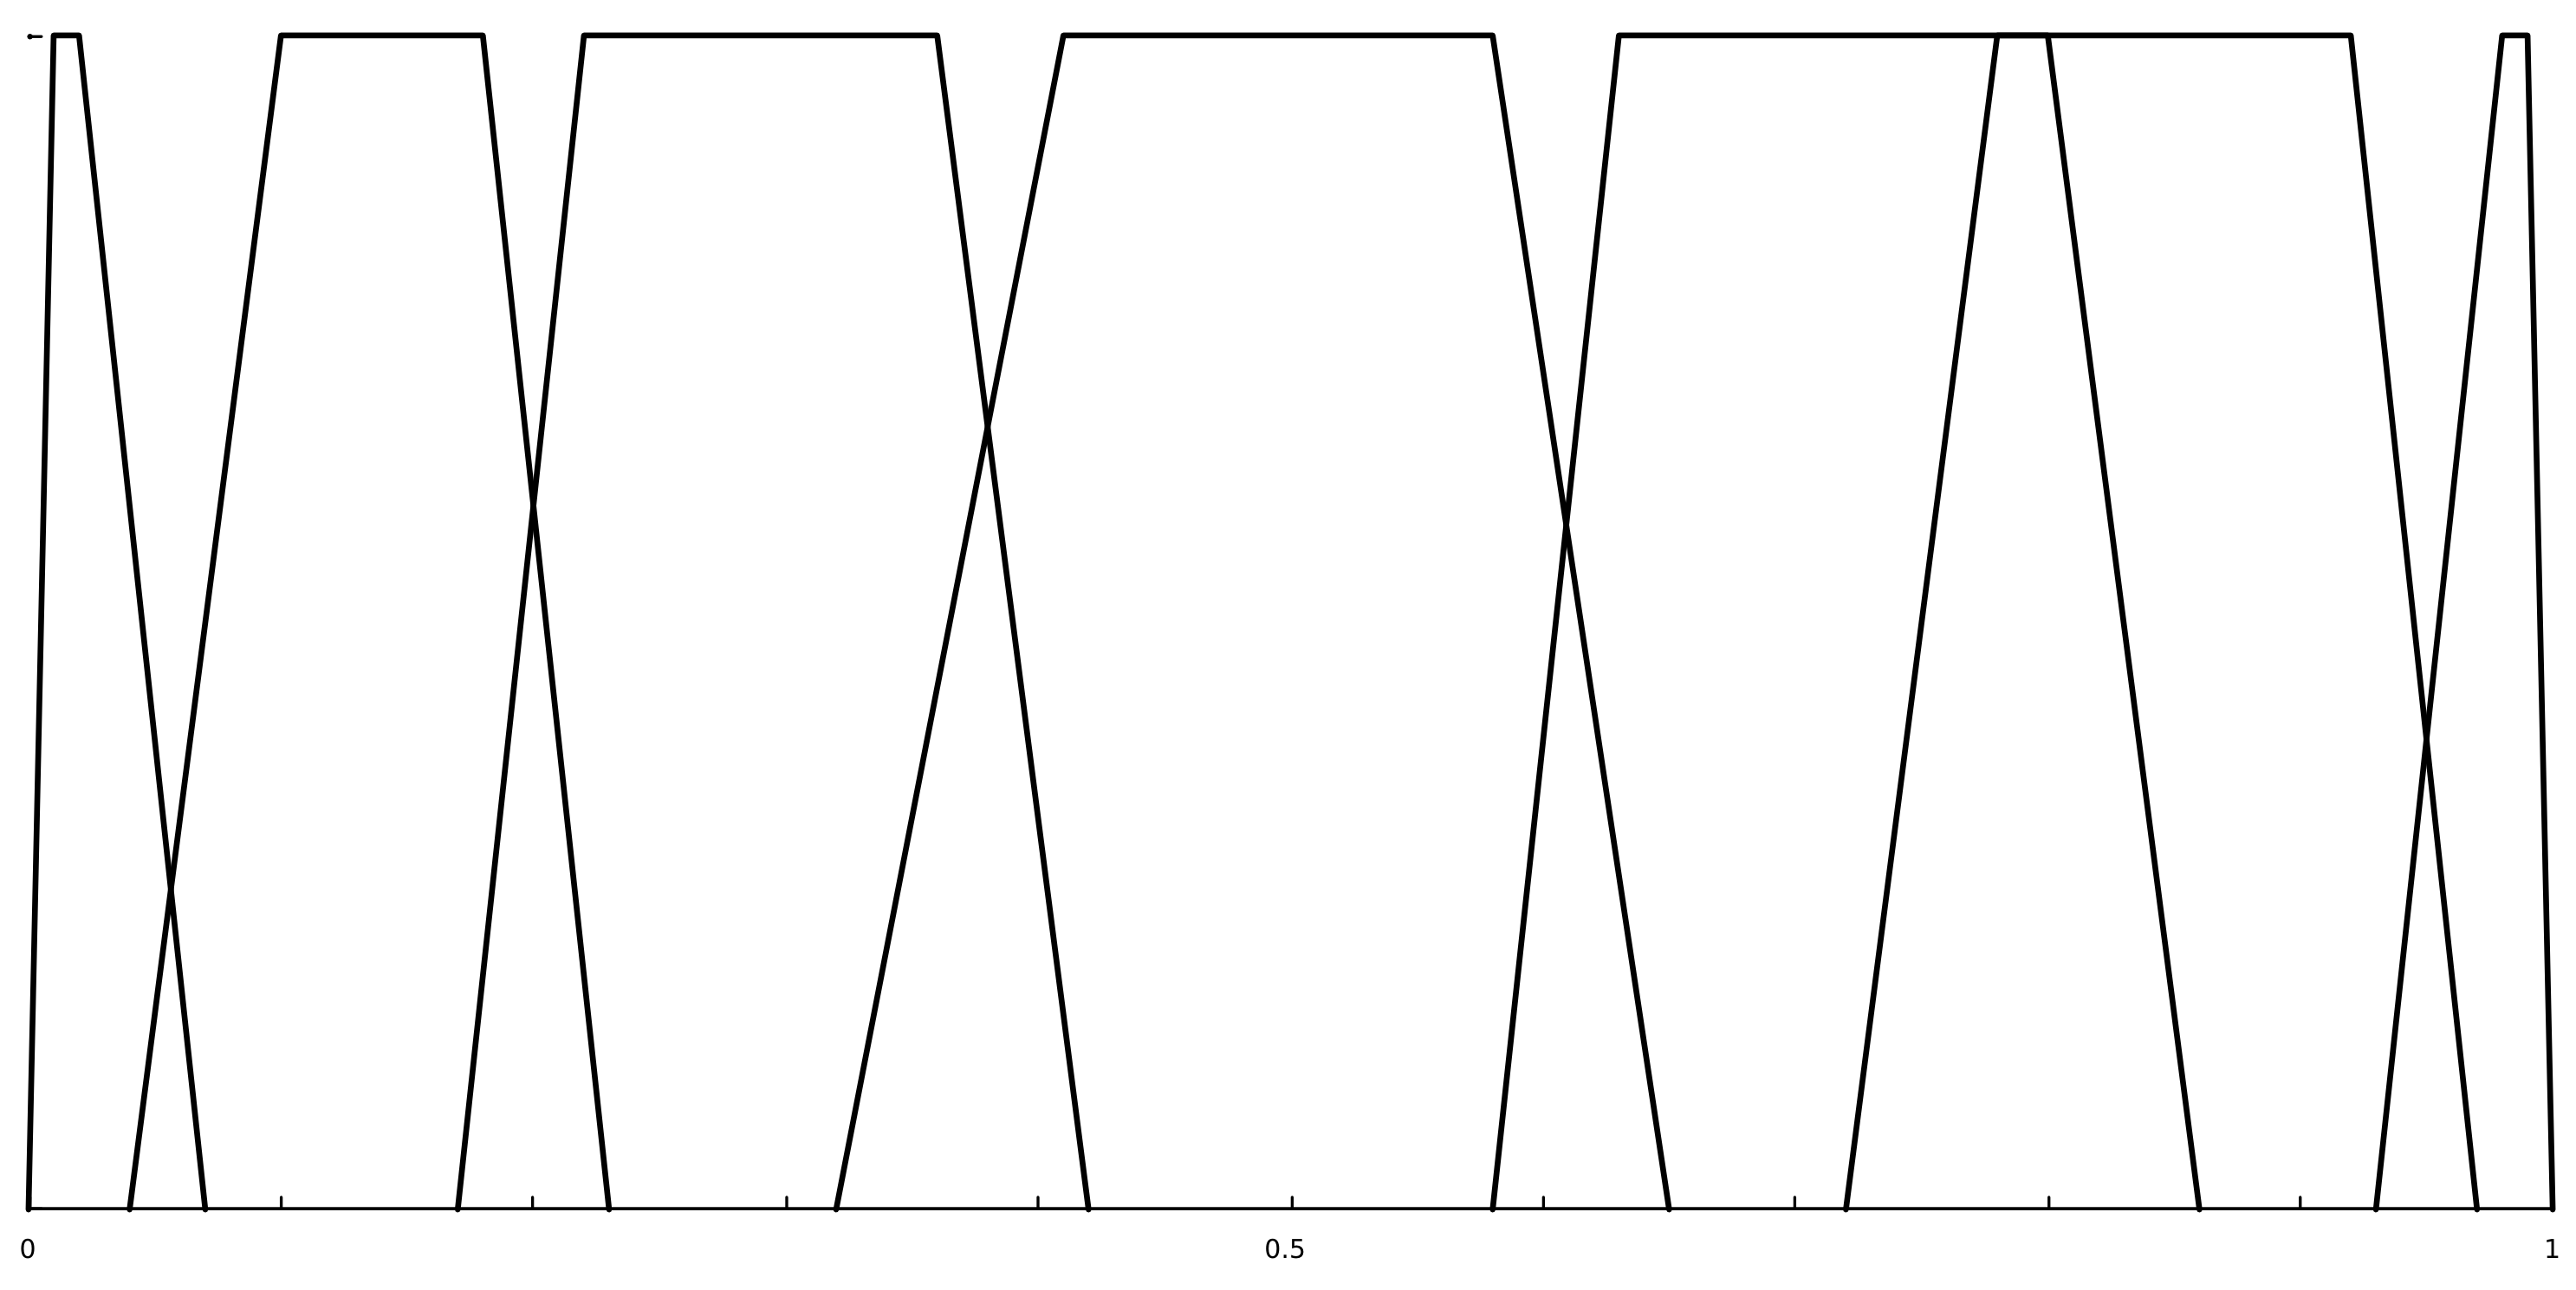
\includegraphics[width=\linewidth]
    {chapters/preferences/zbior_termow}
  \caption{Rozkład dziewięciu termów lingwistycznych}
  \label{fig:rozklad_dziewieciu_termow_lingwistycznych}
\end{figure}
Ze względu na to, że oceny lingwistyczne są przybliżonymi wartościami podanymi
przed decydentów, można uznać, że trapezowe funkcje przynależności są
wystarczające dobre, aby uchwycić niepewność oceny w procesie decyzyjnym.
Potrzebny jest również zbiór termów definiujący granularność niepewności. W
literaturze proponuje się zbiory o nieparzystej liczbie elementów rozłożonych
symetrycznie. Okazuje się również, że granularność, czyli moc zbioru, nie
powinna przekraczać 11 elementów. Dzięki temu unika się uzyskania zbyt
dokładnych wyników, co może być niemożliwe lub niepotrzebne. Co więcej, wybrany
zbiór powinien spełniać następujące warunki:
\begin{enumerate}[1)]
  \item Uporządkowanie
  \item Operator negacji
  \item Operator maksimum
  \item Operator minimum
\end{enumerate}

Przykładem może być następujący zbiór termów lingwistycznych przedstawiony
graficznie na rysunku \ref{fig:rozklad_dziewieciu_termow_lingwistycznych}
(pierwsze dwa parametry oznaczają przedział w którym wartość funkcji
przynależności jest 1, natomiast trzeci i czwarty parametr oznaczają lewą i
prawą szerokość rozkładu):

\begin{tabular}{lll}
P 	&	Pewne				 &	$(1, 1, 0, 0)$ \\
BM 	&	Bardzo Możliwe	 	 &	$(0.98, 0.99, 0.05, 0.01)$ \\
M 	&	Możliwe 			 &	$(0.78, 0.92, 0.06, 0.05)$ \\
ZS 	&	Znacząca Szansa 	 &	$(0.63,0.80,0.05,0.06)$ \\
MB 	&	Może Być 			 &	$(0.41, 0.58, 0.09, 0.07)$ \\
MS 	&	Mała Szansa			 &	$(0.22, 0.36, 0.05, 0.06)$ \\
BMS &	Bardzo Mała Szansa 	 &	$(0.1,0.18, 0.06, 0.05)$ \\
BMM &	Bardzo Mało Możliwe	 &	$(0.01, 0.02, 0.01,0.05)$ \\
N 	&	Niemożliwe 			 &	$(0, 0, 0, 0)$
\end{tabular}

\begin{figure}[ht]
  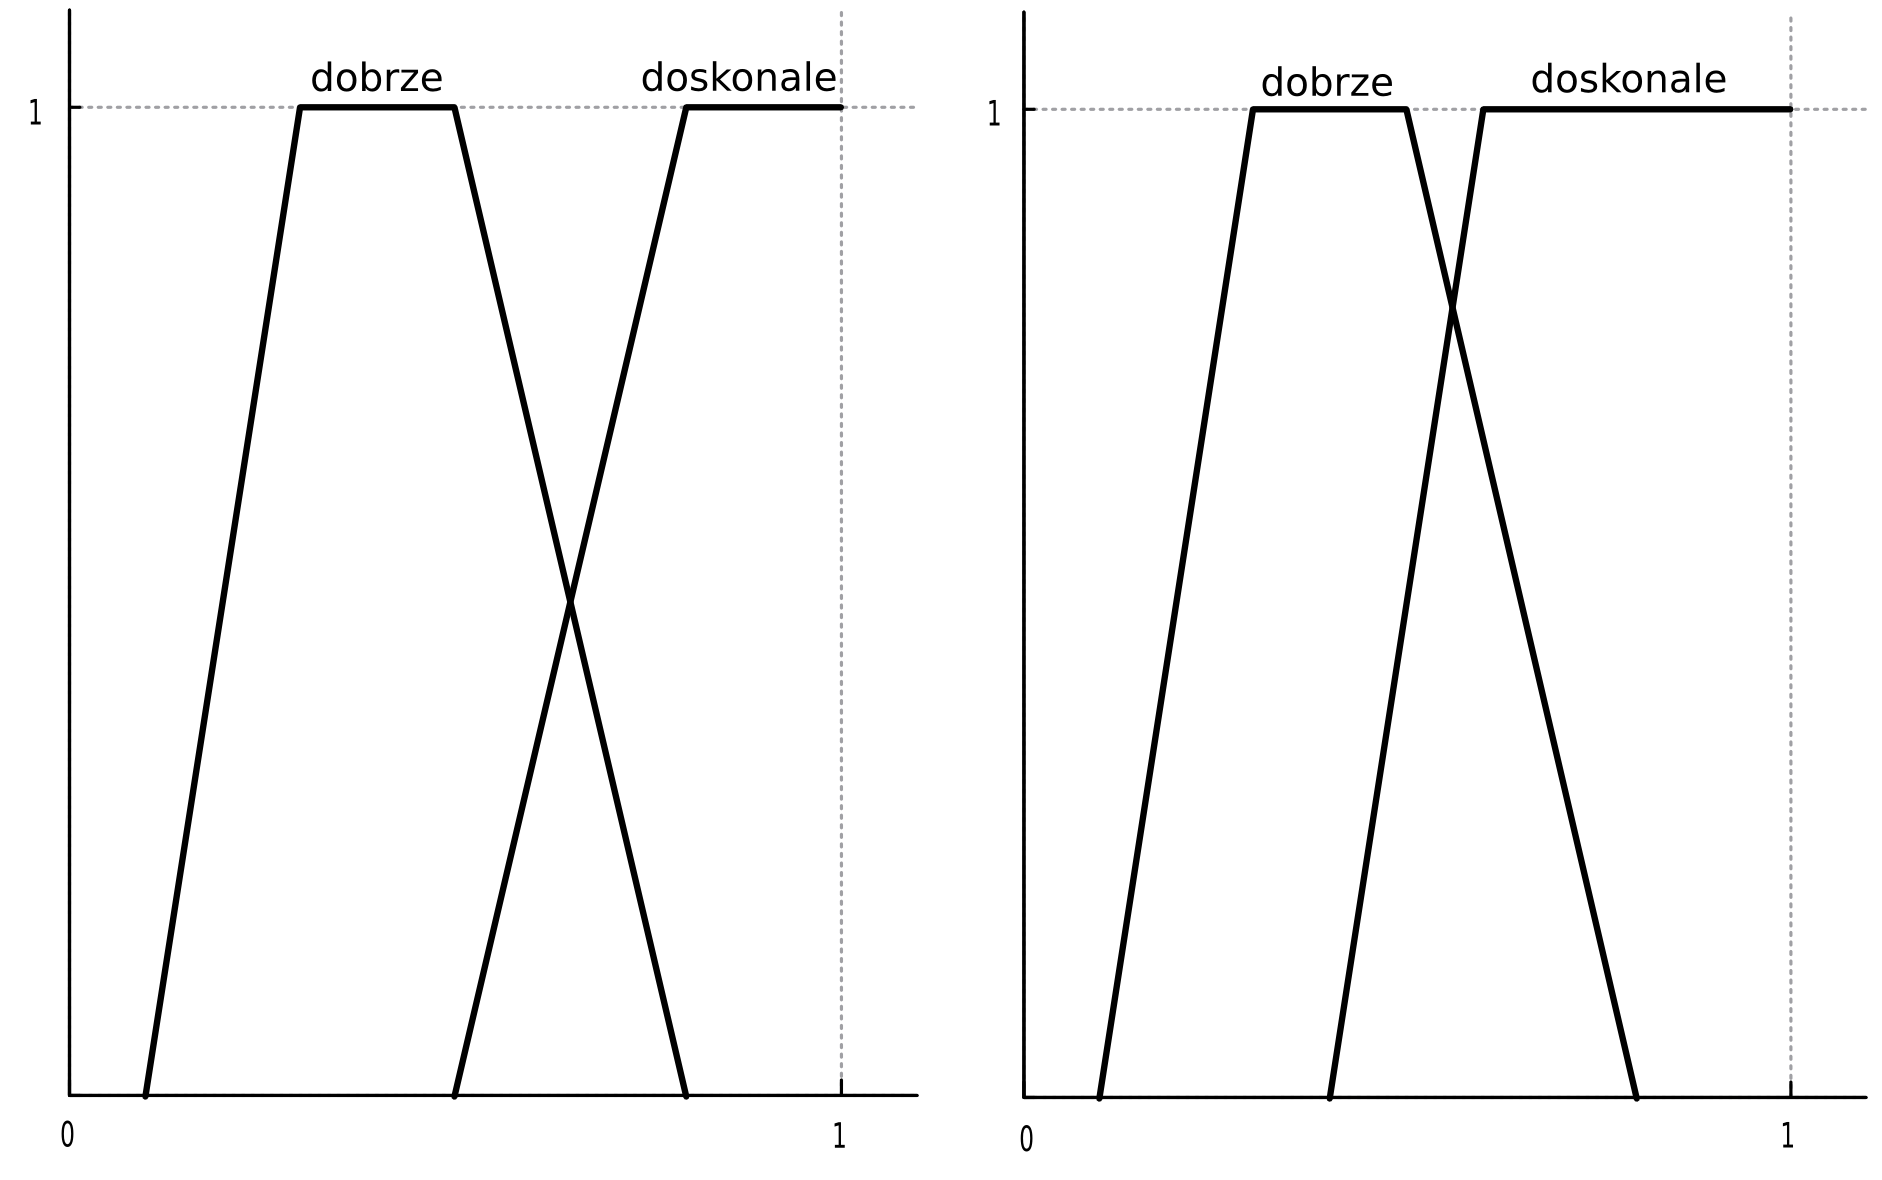
\includegraphics[width=\linewidth]
    {chapters/preferences/rozklad_podobnych_zmiennych}
  \caption{Podobne zmienne lingwistyczne}
  \label{fig:podobne_zmienne_lingwistyczne}
\end{figure}
Okazuje się, że nie można założyć, że wszyscy zgadzają się na takie same funkcje
przynależności przypisane do termów i nie ma jednego uniwersalnego rozkładu. Dla
przykładu można rozważyć dwie bardzo podobne koncepcje przedstawione na rysunku
\ref{fig:podobne_zmienne_lingwistyczne}, które z matematycznego punktu
widzenia bardzo się różnią. Powszechnie przyjmuje się i akceptuje, że
dostrojenie funkcji przynależności jest jednym z ważniejszych elementów w
kontroli procesu. Dobrze jest dostarczyć mechanizm pozwalający ekspertom na
takie dostrojenie, jednak na potrzeby tej pracy przyjmuje się środowisko, w
którym eksperci zgadzają się na odgórnie narzucony zestaw termów lingwistycznych
ze względu na to, że zmienna lingwistyczna ma służyć zapewnieniu środków
umożliwiających zbliżoną charakterystykę nieprecyzyjnej oceny preferencji.

\subsection{Niesymetryczna zmienna lingwistyczna}
Wiele problemów można oceniać przy pomocy opisanych wcześniej zmiennych
lingwistycznych, których termy są równomiernie i symetrycznie rozłożone.
Istnieją jednak problemy, które muszą korzystać ze zmiennych lingwistycznych,
które nie mają takich właściwości, to znaczy mają nierównomiernie i
niesymetrycznie rozłożony zbiór termów. Tego typu zmienne lingwistyczne nazywane
są niesymetrycznymi zmiennymi lingwistycznymi (rysunek
\ref{fig:niesymetryczna_zmienna}).
\begin{figure}[ht]
  
\includegraphics[width=\linewidth]
    {chapters/preferences/niesymetryczna_zmienna}
  \caption{Niesymetryczny rozkład termów}
  \label{fig:niesymetryczna_zmienna}
\end{figure}

W pracy dotyczącej informacji niesymetrycznej, Alonso et al. zaproponowali nowy
model radzenia sobie z niesymetrycznymi zmiennymi lingwistycznymi w procesie
podejmowania decyzji. W tym celu wykorzystana została tak zwana hierarchia
lingwistyczna, czyli zbiór poziomów, gdzie każdy poziom reprezentuje zbiór
termów lingwistycznych o odpowiedniej granularności. Każdy poziom oznaczany jest
jako $l(t, n(t))$, gdzie $t$ to numer porządkowy poziomu, a $n(t)$ to liczba
termów na poziomie $t$. Przez $S^{n(t)} = \{s^{n(t)}_0, \dotsc,
s^{n(t)}_{n(t)-1}\}$ oznacza się zbiór termów lingwistycznych na poziomie $t$.
Graficzny przykład hierarchii lingwistycznej pokazano na rysunku
\ref{fig:hierarchia_lingwistyczna}.
\begin{figure}[hb]
  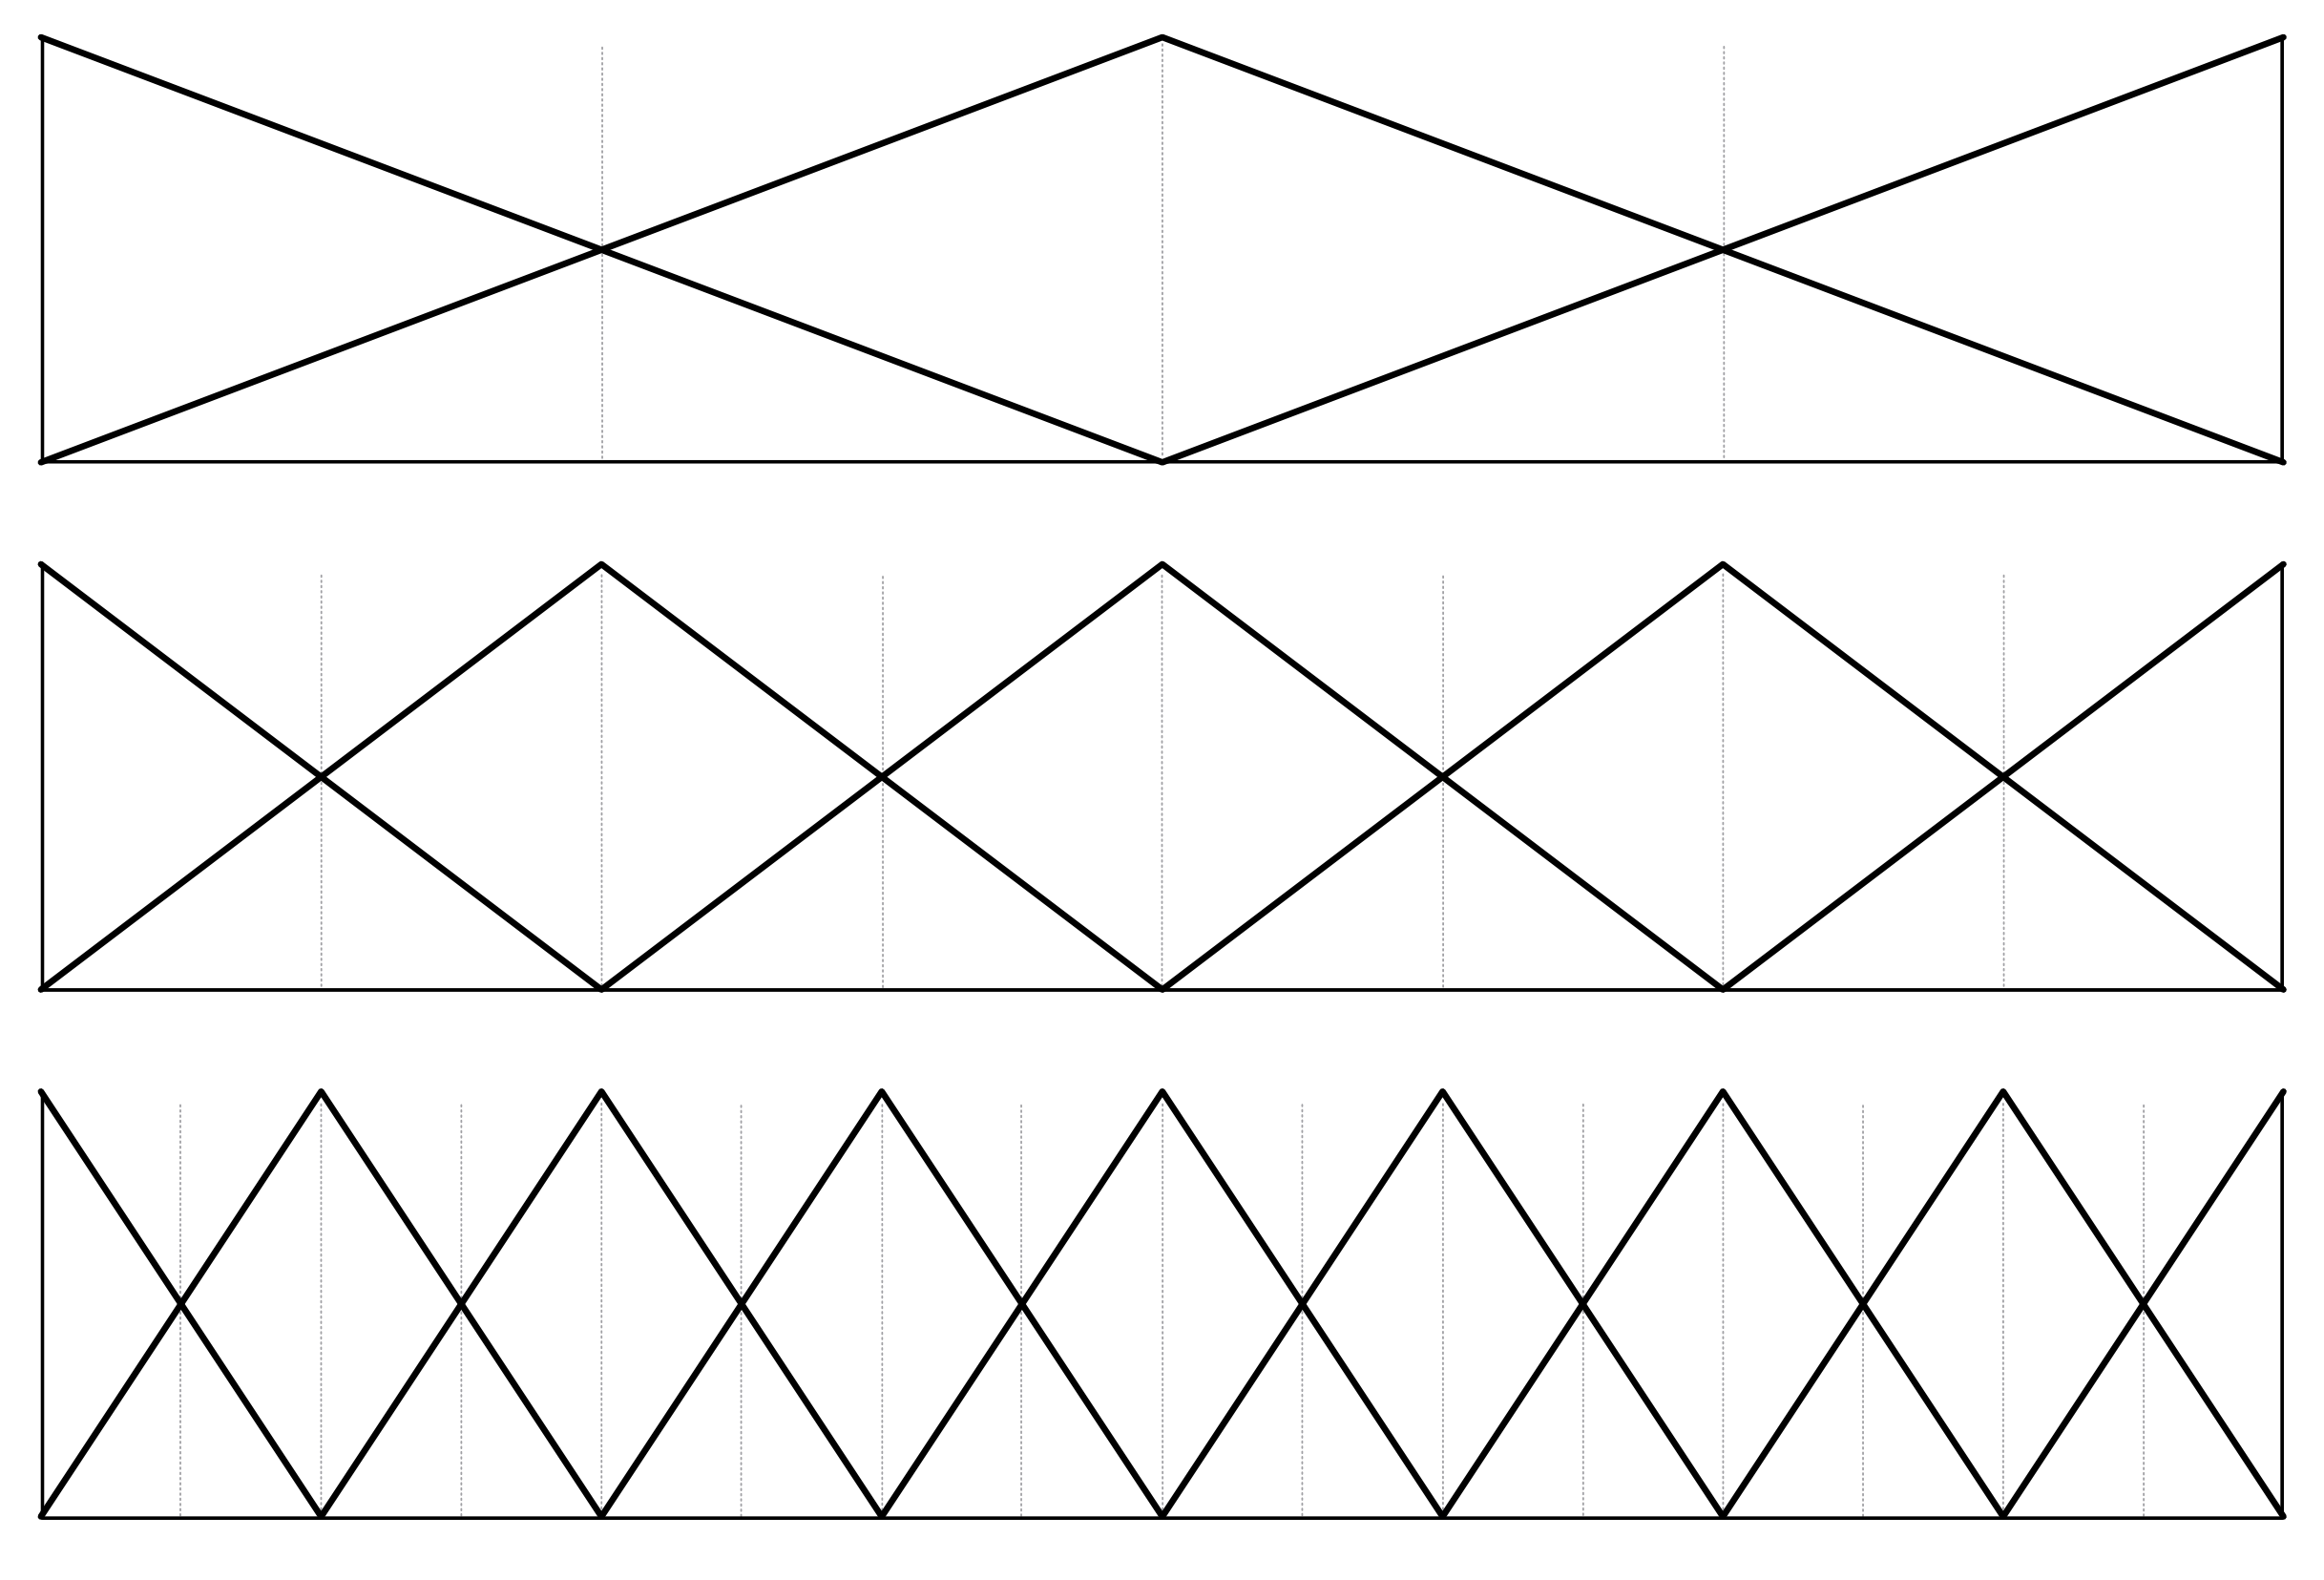
\includegraphics[width=\linewidth]
    {chapters/preferences/hierarchia_lingwistyczna}
  \caption{Przykładowa hierarchia lingwistyczna}
  \label{fig:hierarchia_lingwistyczna}
\end{figure}

W omawianym w tej pracy modelu podejmowania decyzji grupowej możliwe jest użycie
różnych zaprezentowanych powyżej sposobów wprowadzania preferencji. Z tego
powodu potrzebna jest transformacja z jednej metody na drugą. W przypadku
niesymetrycznej zmiennej lingwistycznej wygodne okazuje się przedstawienie jej
przy pomocy klasycznej zmiennej lingwistycznej. Najprostsza procedura wykonująca
tą czynność przy użyciu hierarchii lingwistycznej wygląda następująco:
\begin{enumerate}[i.]
  \item Znajdź poziom $t^-$ w $LH$ (ang. Linguistic Hierarchy) reprezentujący
  podzbiór termów $S^L_{UN}$ na lewo od środkowego termu w niesymetrycznym
  zbiorze termów lingwistycznych $S_{UN}$. Znaleziony poziom $LH$ powinien
  odpowiadać rozkładowi termów w $S^L_{UN}.$
  \item Znajdź poziom $t^+$ w $LH$ reprezentujący podzbiór termów $S^R_{UN}$ na
  prawo od środkowego termu ze zbioru $S_{UN}.$
  \item Środkowy term zbioru $S_{UN}$ przedstaw używając środkowych
  termów z poziomów $t^-$ i $t^+.$
\end{enumerate}

Okazuje się, że pojawia się problem, kiedy nie istnieje poziom $t^-$ lub $t^+$ w
$LH$ reprezentujący, odpowiednio, $S^L_{UN}$ lub $S^R_{UN}$. Dlatego Alonso et
al. zaprezentowali algorytm, który zakłada brak poziomu $t^-$, jak na rysunku
\ref{fig:niesymetryczna_zmienna} (przez analogię można napisać algorytm dla
$t^+$):
\begin{enumerate}[i.]
  \item Reprezentacja $S^L_{UN}\colon$
  \begin{enumerate}[(a)]
    \item Zidentyfikuj środkowy term $S^L_{mid}$ w $S^L_{UN}$.
    \item Znajdź poziom $t^-_2$ po lewej stronie zbiorów $LH^L$, który odpowiada
    lewemu podzbiorowi termów z $S^L_{UN}$, gdzie $LH^L$ oznacza lewą część
    $LH$.
    \item Znajdź poziom $t^+_2$ po prawej stronie zbiorów $LH^L$, który
    odpowiada prawemu podzbiorowi termów z $S^L_{UN}$.
    \item Przedstaw środkowy term $S^L_{mid}$ używając poziomów $t^-_2$ i
    $t^+_2$.
  \end{enumerate}
  \item Znajdź poziom $t^+$ w $LH$ reprezentujący podzbiór termów $S^R_{UN}$.
  \item Środkowy term zbioru $S_{UN}$ przedstaw używając środkowych termów z
  poziomów $t^+$ i $t^+_2$.
\end{enumerate}
\begin{figure}[ht]
  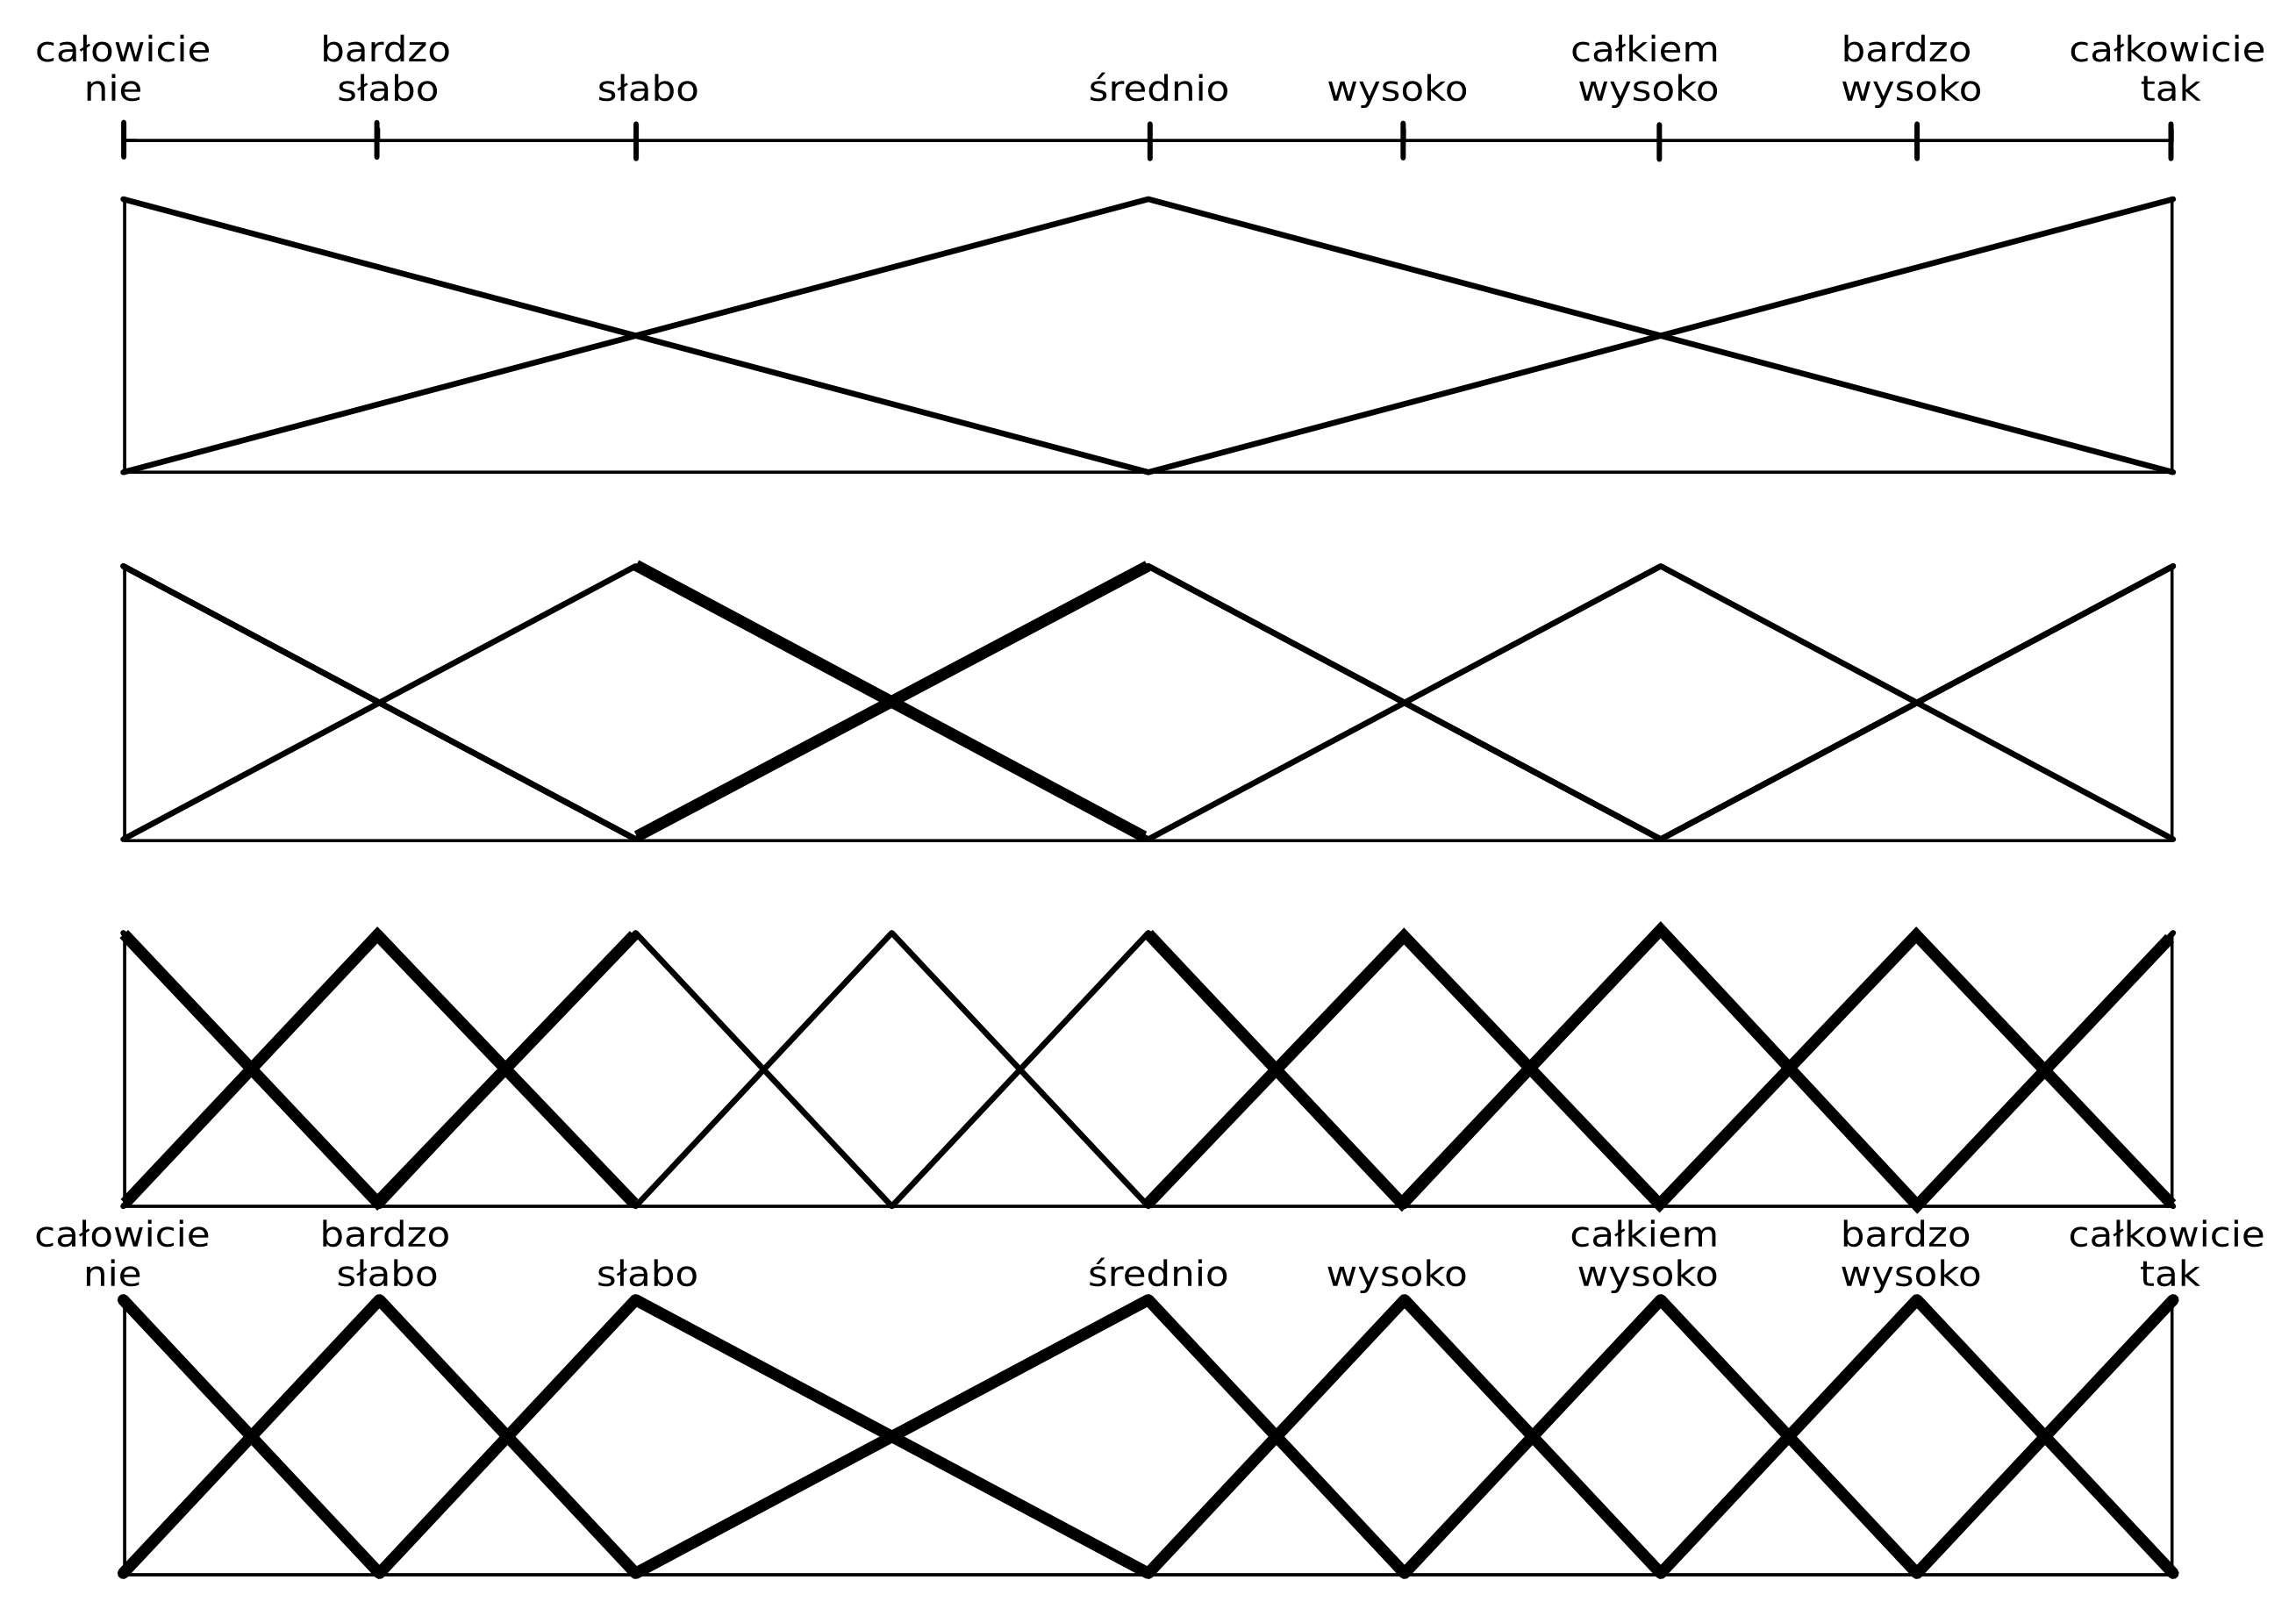
\includegraphics[width=\linewidth]
    {chapters/preferences/hierarchia_lingwistyczna_przyklad}
  \caption{Reprezentacja niesymetrycznej zmiennej lingwistycznej}
  \label{fig:hierarchia_lingwistyczna_przyklad}
\end{figure}
Przykład działania algorytmu został przedstawiony na rysunku
\ref{fig:hierarchia_lingwistyczna_przyklad}, na którym jest reprezentacja
niesymetrycznego zbioru termów lingwistycznych $S_{UN} = \{ N, VL, L,$ $M, H, 
QH, VH, T \}$ z rysunku \ref{fig:niesymetryczna_zmienna} dla hierarchii
lingwistycznej $LH$ z rysunku \ref{fig:hierarchia_lingwistyczna}.
W tym przykładzie mamy:
\begin{itemize}
  \item $S^L_{UN} = \{N,VL,L\},$
  \item $S^L_{mid} = L,$
  \item $LH^L = \{s_0^{n(1)}\} \cup \{s_0^{n(2)}, s_1^{n(2)}\} \cup
  \{s_1^{n(3)}, s_2^{n(3)}, s_3^{n(3)}\}.$
\end{itemize}

	
	\chapter{System wspomagania decyzji grupowej}
	
\section{Organizacja pracy grupy}
Członkowie grupy są ludźmi. Jako ludzie, szukamy na około, tracimy główny wątek 
dyskusji, przywiązujemy się do naszych pomysłów. Nawet jeśli bardzo się staramy,
żeby utrzymać koncentrację i „pozostać na torze”, nie możemy zmienić faktu, że 
jesteśmy indywidualnościami o różnych punktach widzenia. Podczas dyskusji, 
każdy z członków grupy powinien mieć okazję do przedstawienia swoich propozycji 
rozwiązań oraz oceny innych alternatyw. W większości przypadków dochodzi do tak 
zwanej ,,burzy mózgów''. Bardzo dużo osób obawia się, że proces wymknie się spod
kontroli i zostanie zatracony sens dyskusji. Niemniej jednak, coś co wydaje się 
być chaosem, może okazać się wstępem do kreatywności. Dlatego w modelu 
podejmowania decyzji grupowej powinien być czas na tak zwaną ,,strefę
rozbieżną'' oraz ,,strefę zbieżną'', a pomiędzy nimi ,,strefę jęku''. Są to
elementy, które większość isniejących modeli pomija, a tak naprawdę to właśnie
dyskusja jest kluczem prowadzącym do osiągnięcia konsensus.

Strefa rozbieżna to miejsce na myślenie w coraz to szerszym zakresie. Na samym 
początku grupa przedstawia oczywiste lub dobrze znane (na przykład z 
poprzednich problemów) rozwiązania. Jeśli okaże się to wystarczające to 
wyszukiwanie alternatyw może się zakończyć w tym miejscu. Jednakże istnieją 
problemy, na które nie ma prostej odpowiedzi i grupa musi wyjść poza pewne ramy 
w poszukiwaniu szerszego spektrum możliwości. To jest miejsce, do którego wiele 
grup nie dociera. Boimy się wychodzić poza utarte schematy, bo możemy zostać 
skrytykowani lub, w najlepszym wypadku, zignorowaniu. To jest również jedno z 
tych miejsc, w których idealnie sprawdza się system informatyczny, w którym 
zapewniona jest anonimowość przedstawianych rozwiązań.

Teoretycznie, w pewnym momencie czasu, grupa sama powinna zacząć myśleć w 
kierunku uporządkowania dyskusji i wyboru ostatecznych rozwiązań, czyli  przejść
do ,,strefy zbieżnej''. Niestety, w prawdziwym życiu jest inaczej. W praktyce,
przejście ze strefy wyrażania swoich propozycji do strefy rozumienia perspektyw 
pozostałych członków grupy jest bardzo trudne. Ludzie mogą czuć się przeciążeni,
zdezorientowani, zniechęceni. Mogą pojawić się stwierdzenia o utknięciu w 
miejscu, o traceniu czasu, osoby  z silniejszą pozycją mogą nakłaniać do 
zakończenia procesu i wybraniu ich opcji.

Członkowie grupy, zanim zaczną rozumieć punkt widzenia innych członków, muszą 
przejść przez fazę walki o integrację nowych, innych podejść do problemu ze 
swoim samym. Jest to tak zwana „strefa jęku”. Jest to miejsce na dyskusje, a 
nawet kłótnie. Sam fakt świadomości, że w modelu jest miejsce na wymianę zdań, 
może znacząco przyczynić się do osiągnięcia konsensusu przez grupę.

\section{Zasada działania}
Zaprponowany w tej pracy system wspomagania decyzji grupowej ma za zadanie
poprowadzić grupę przez cały proces oraz ułatwić osiągnięcie konsensusu i
wybranie optymalnego rozwiązania. W związku z opisaną powyżej organizacją pracy
grupy, ważnym elementem systemu jest moduł dyskusji. Eksperci mają możliwość
przedstawiać swoje alternatywy oraz, oprócz zwykłego głosowania, wyrażać opinię
i rozmawiać na temat problemu i rozwiązań. Dzięki temu, grupa może poczuć się
jak na rzeczywistym spotkaniu. Prowadzi to do kolejnego założenia.

System umożliwia dynamiczną dyskusję nad problemem bez konieczności gromadzenia 
ekspertów w jednym miejscu i czasie. Aby uczestniczyć w podjęciu decyzji 
wymagane jest tylko urządzenie z dostępem do internetu oraz przeglądarką 
internetową. Zastosowanie najnowszych technologii mobilnych rozszerza możliwości
podejmowania decyzji, na przykład możliwe jest osiągnięcie konsensusu wśród 
ekspertów rozlokowanych w różnych krajach i strefach czasowych.

Szczegółowy opis działania systemu na przykładach opisany jest w kolejnym 
rozdziale, natomiast poniżej przedstawiony został model teoretyczny 
wykorzystujący techniki przedstawione wcześniej.

\section{Model teoretyczny}
Opisywany model teoretyczny bazuje na modelu przedstawionym w pracy Herrera
\todo{biblio: Herrera Web DSS} oraz wprowadza kilka udoskonaleń.

Jednym z nich jest zrezygnowanie z podejścia iteracyjnego. Oznacza to dużo
większą dynamikę oraz naturalność procesu. W klasycznym podejściu, system czeka
aż wszyscy eksperci biorący udział w procesie wprowadzą swoje preferencje
względem alternatyw, a sam zbiór ekspertów jest stały. W przypadku braku
informacji od któregoś z członków zespołu cały proces wspomagania decyzji
zostaje wstrzymany. 
Lepszym rozwiązaniem jest uruchomienie etapów schematu modelu w momencie
otrzymania pierwszego, nawet niepełnego, zbioru preferencji od jednego z
ekspertów. System obliczając poziom konsensusu bierze pod uwagę ilość
głosujących ekspertów do ilości wszystkich ekspertów biorących udział w
procesie. Pozwala to zapewnić płynność procesu oraz ułatwia dynamiczne
zarządzanie zbiorem ekspertów.

Zrezygnowanie z podejścia iteracyjnego w naturalny sposób pociąga kolejną
modyfikację. W klasycznych modelach na początku ustalana jest maksymalna liczba
iteracji, po której system powinien zakończyć działanie bezwzględu na wynik.
Ze względu na specyfikę zagadnienia, system powinien jedynie wspomagać grupę i
sugerować działania, ale nie podejmować decyzji samodzielnie. To zespół powinien
decydować, czy osiągniety konsensus jest satysfakcjonujący czy nie, dlatego
proces wspierania decyzji domyślnie jest nieskończony w czasie.

Struktura proponowanego modelu grupowego podejmowania decyzji składa się z
sześciu etapów opisanych w kolejnych punktach:
\begin{itemize}
  \item etap unifikowania,
  \item etap selekcji,
  \item etap konsensusu,
  \item etap dynamicznego wyboru alternatyw,
  \item etap informacji zwrotnej,
  \item etap dynamicznej selekcji ekspertów.
\end{itemize}

\missingfigure{Schemat modelu}

\subsection{Etap unifikowania}
Aby sprostać wymaganiom użytkowników oraz zapewnić duży stopień swobody w
wyrażaniu swoich preferencji, eksperci mogą wprowadzać swoje oceny na temat
alternatyw przy pomocy dowolnie przez siebie wybranej metody wprowadzania
preferencji opisanej w rozdziale na temat sposobów prezentacji preferencji. W
związku z tym, konieczne jest zunifikowanie uzyskanych informacji przed
przejściem do dalszych etapów. Ze względu na użyteczność i wygodę w dalszym
przetwarzaniu informacji, szczególnie przy agregacji ocen ekspertów w ocenę
zbiorczą, do reprezentacji preferencji w dalszych etapach wybrano rozmytą
relację preferencji [9]. Aby jednak było możliwe zamienianie poszczególnych
metod na relację rozmytą, potrzebne są funkcje transformacji.

\subsubsection{Funkcja użyteczności a relacja rozmyta}
W przypadku funkcji użyteczności zakłada się, że każdy ekspert $e_k$ podaje
swoje preferencje dla zbioru alternatyw $\mathcal{X}$ jako zbiór wartości
użyteczności $U^k = \{ u^k_i; i=1,\dotsc,n\}, u^k_i \in [0,1]$, gdzie
$u^k_i$ reprezentuje wartość użyteczności alternatywy $x_i$ daną przez eksperta
$e_k$. Dla każdego zbioru $U^k$ bez straty ogólności, można założyć, że im
wyższa wartość tym bardziej dana alternatywa odpowiada ekspertowi.

Dowolna możliwa funkcja transformacji $f$ musi ustalić dla eksperta $e_k$ jego
stopień preferencji alternatywy $x_i$ nad $x_j$ ($p^k_{ij}$) tylko w zależności
od wartości $u^k_i$ oraz $u^k_j$, to znaczy 
\begin{equation}
p^k_{ij} = h(u^k_i, u^k_j).
\end{equation}
Funkcja transformacji $f$ musi zakładać również, że większa wartość $u^k_i$
pociąga większą wartość $p^k_{ij}$, a większa $u^k_j$ to mniejsza $p^k_{ij}.$

\begin{theorem}
Dla każdego zbioru wartości użyteczności $U^k = \{ u^k_1, \dotsc, u^k_n \}$ nad
zbiorem alternatyw $\mathcal{X} = x_1, \dotsc, x_n\}$, stopień preferencji
alternatywy $x_i$ nad $x_j$ ($p^k_{ij}$) otrzymywany jest ze współczynnika
$^{u^k_i}/_{u^k_j}$ przy użyciu następującej funkcji transformacji:
\begin{equation}
p^k_{ij} = f(u^k_i, u^k_j) =
  \left\{ 
	\begin{array}{ll}
	  \frac{s(u^k_i)}{s(u^k_i) + s(u^k_j)} & \quad \textrm{jeżeli } (u^k_i,u^k_j)
	  \neq 0
	  \\
      \frac{1}{2} & \quad \textrm{jeżeli } (u^k_i,u^k_j) = 0
  	\end{array} 
  \right. (i \neq j) .
\end{equation}
gdzie $s : [0,1] \rightarrow \mathbb{R}^+$ jest dowolną niemalejącą i ciągłą
funkcją spełniającą $s(0) = 0.$
\end{theorem}

Przykładowa funkcja spełniająca powyższe twierdzenie zaproponowana w [10] oraz
wykorzystywana w przedstawianym systemie wygląda następująco:
\begin{equation}
f^1(u^k_i,u^k_j) = \frac{(u^k_i)^2}{(u^k_i)^2 + (u^k_j)^2}
\end{equation}

\subsubsection{Uporządkowanie alternatyw a relacja rozmyta}
W tym przypadku, ekspert $e_k$ podaje swoje preferencje jako uporządkowanie
alternatyw $O^k = \{o^k(1), \dotsc, o^k(n)\}$. Dla każdego zbioru $O^k$ bez
straty ogólności, można założyć, że im mniejsza pozycja alternatywy w
uporządkowaniu tym większa satysfakcja eksperta. Dla przykładu, uporządkowanie
zbioru alternatyw $\mathcal{X} = \{x_1,x_2,x_3,x_4\}$ przez eksperta $e_k$ to
$O^k = \{3,1,4,2\}.$ Oznacza to, że alternatywa $x_2$ jest najlepsza dla
eksperta, a $x_3$ najgorsza.

Dowolna możliwa funkcja transformacji $f$ musi ustalić dla eksperta $e_k$ jego
stopień preferencji alternatywy $x_i$ nad $x_j$ ($p^k_{ij}$) tylko w zależności
od wartości $o^k(i)$ oraz $o^k(j)$, to znaczy
\begin{equation}
p^k_{ij} = f(o^k(i), o^k(j)).
\end{equation}
Funkcja transformacji $f$ musi zakładać również, że większa wartość $o^k(i)$
pociąga mniejszą wartość $p^k_{ij}$, a większa $o^k(j)$ to większa $p^k_{ij}$.

\begin{theorem}
Dla każdego uporządkowania alternatyw $O^k = \{o^k(1), \dotsc, o^k(n)\}$ nad
zbiorem alternatyw $\mathcal{X} = \{x_1,\dotsc,x_n\}$, stopień preferencji
alternatywy $x_i$ nad $x_j$ ($p^k_{ij}$) otrzymywany jest przy użyciu
następującej funkcji transformacji:
\begin{equation}
p^k_{ij} = f(o^k(i),o^k(j)) = \frac{1}{2} [1 + F(o^k(j) - o^k(i)) - F(o^k(i) -
o^k(j))].
\end{equation}
gdzie $F$ jest dowolną funkcją niemalejącą.
\end{theorem}

Przykładowa funkcja spełniająca powyższe twierdzenie zaproponowana w [10] oraz
wykorzystywana w przedstawianym systemie wygląda następująco:
\begin{equation}
f^2(u^k_i,u^k_j) = \frac{(u^k_i)^2}{(u^k_i)^2 + (u^k_j)^2}.
\end{equation}

\subsubsection{Multiplikatywna relacja preferencji a relacja rozmyta}
Ekspert $e_k$ podaje swoje preferencje poprzez multiplikatywną relację
preferencji $A^k = [a^k_{ij}]$. W ogólności, zgodnie z propozycją Saaty'ego,
jeżeli
$$A' = \{ A^k = [a^k_{ij}] : a^k_{ij} \cdot a^k_{ji} = 1, a^k_{ij} \in
[^1/_9,9], k= 1, \dotsc, m \}$$ 
jest multiplikatywną relacją preferencji oraz
$$P' = \{ P^k = [p^k_{ij}] : p^k_{ij} + p^k_{ji} = 1, p^k_{ij} \in
[0,1], k= 1, \dotsc, m \}$$
jest rozmytą relacją preferencji, to szukana funkcja transformacji ma postać:
\todo{FIXME: niepoprawny wzor}
$$P' = \{ P^k = [p^k_{ij}] : p^k_{ij} + p^k_{ji} = 1, p^k_{ij} \in
[0,1], k= 1, \dotsc, m \}.$$ 
Ta klasa funkcji jest równoważna klasie funkcji spełniających
$$F : A' \rightarrow P',\; F(A^k) = P^k \; \forall k,$$
$$ f(x)+f(\frac{1}{x})=1 \text{ oraz } f(9)=1.$$
Funkcja $f$ może być zapisana w postaci $f(x) = \frac{1}{2} + h(x)$, co
implikuje $h(x) + h(\frac{1}{x}) = 0 $ oraz $h(9) = \frac{1}{2}.$

Z drugiej strony, ogólne rozwiązanie równania funkcjonalnego $l(x \cdot y) =
l(x) + l(y)$ na przedziale $[1, \infty]$ to $l(z) = C \cdot \ln z, C \in
\mathbb{R}.$
W tej sytuacji, zachodzi $y = \frac{1}{x}$ i podstawiając $x = 1$ dostajemy $0
= h(1) + h(1) = 2 \cdot h(1) = 2 \cdot h(x \cdot y).$ Funkcja $h$ spełnia
$h(x \cdot y) = h(x) + h(y)$, czyli $l(z) = C \cdot \ln z, C \in \mathbb{R}.$
Skoro $h(9) = \frac{1}{2}$, to $C = \frac{1}{2 \cdot \ln 9}$ oraz $h(z) =
\frac{1}{2} \frac{\ln z}{\ln 9} = \frac{1}{2} \log_9 z.$

Podsumowując, w [7] otrzymano następujące twierdzenie:
\begin{theorem}
Dla każdej relacji preferencji $A^k = [a^k_{ij}]$ nad zbiorem alternatyw
$\mathcal{X} = \{x_1,\dotsc,x_n\}$, stopień preferencji alternatywy $x_i$ nad
$x_j$ ($p^k_{ij}$) otrzymywany jest przy użyciu następującej funkcji
transformacji:
\begin{equation}
p^k_{ij} = f^3(a^k_{ij}) = \frac{1}{2}(1 + \log_9 a^k_{ij}).
\end{equation}
\end{theorem}

\subsubsection{Niepełna ocena}
Zazwyczaj modele grupowego podejmowania decyzji zakładają, że ekspert jest
zawsze w stanie podać swoje preferencje względem wszystkich alternatyw. Jest to
bardzo optymistyczne założenie, ponieważ w trakcie trwania dyskusji oraz ze
względu na dynamikę zbioru alternatyw nie zawsze istnieje taka możliwość. Z
braku czasu, niewystarczającej wiedzy lub danych, albo z innych indywidulanych
przyczyn eksperci mogą wyrazić swoje preferencje względem tylko części
alternatyw. W takich sytuacjach mówi się o \emph{niepełnej rozmytej relacji
preferencji}.

W pracy Alonso, Cabrerizo et al. (2009) została przedstawiona metoda estymacji
brakujących wartości. Zapewnia ona addytywną konsystencję z preferencjami
podanymi przez eksperta. Jest to iteracyjna procerdura, która w całości została
zaadoptowana w tej pracy.

\subsection{Proces selekcji: agregacja}
Jest to faza, w której definiowana jest zbiorcza rozmyta relacja preferencji
$P^c = [p^c_{ij}]$, otrzymana poprzez agregację wszystkich indywidualnych
rozmytych relacji preferencji otrzymanych w procesie unifikacji $\{ P^1, P^2,
\dotsc, P^m \}$. Każda wartość $p^c_{ij} \in [0,1]$ reprezentuje stopień
preferencji alternatywy $x_i$ nad $x_j$ według opinii większości ekspertów.
Tradycyjnie, większość oznacza pewną liczbę progową. W tym przypadku, stosowana
jest rozmyta większość wyrażona przez rozmyty kwantyfikator lingwistyczny.

Każda wartość $p^c_{ij}$ jest obliczana przy pomocy operatora agregacji OWA.
Operator OWA odzwierciedla rozmytą większość obliczając wektor wag przy pomocy
kwantyfikatora rozmytego. Zatem zbiorcza rozmyta relacja preferencji otrzymywana
jest w następujący sposób:
\begin{equation}
p^c_{ij} = \Phi_Q(p^1_{ij}, \dotsc, p^m_{ij}).
\end{equation}
gdzie $Q$ jest rozmytym kwantyfikatorem użytym do obliczenia wektora wag dla
operatora OWA $\Phi_Q$.

\subsection{Proces selekcji: eksploatacja}
W tej fazie przekształcana jest globalna informacja o alternatywach w globalny
ranking, z której można uzyskać zbiór rozwiązań. Globalny ranking uzyskuje się
poprzez użycie dwóch stopni wyboru alternatyw: kwantyfikowany stopień dominacji
(QGDD, ang. quantifier guided dominance degree) oraz kwantyfikowany stopień
nie-dominacji (QGNDD, ang. quantifier guided non dominance degree).

Kwantyfikowany stopień dominacji $QGDD_i$ to wielkość dominacji jaką posiada
alternatywa $x_i$ nad pozostałymi w sensie rozmytej większości:
\begin{equation}
QGDD_i = \Phi_Q(p^c_{i1}, p^c_{i2}, \dotsc, p^c_{i(i-1)},p^c_{i(i+1)}, \dotsc,
p^c_{i \cdot n}).
\end{equation}
Ta miara pozwala na zdefiniowanie zbioru dominujących alternatyw z maksymalnym
stopniem dominacji:
\begin{equation}
X^{QGDD} = \{ x_i \in \mathcal{X} : QGDD_i = \sup_{x_j \in \mathcal{X}} QGDD_j
\}.
\end{equation}

Kwantyfikowany stopień nie-dominacji $QGNDD_i$ podaje stopień w jakim każda
alternatywa nie jest zdominowana przez pozostałe alternatywy w sensie rozmytej
większości:
\begin{equation}
QDNDD_i = \Phi_Q(\neg(p^s_{1i}), \neg(p^s_{2i}), \dotsc,
\neg(p^s_{(i-1)i}), \neg(p^s_{(i+1)i}), \dotsc, \neg(p^s_{n \cdot i})).
\end{equation}
gdzie
$p^s_{ji} = 
  \left\{ 
	\begin{array}{ll}
	  0 				  & \quad \textrm{jeżeli } p^c_{ji} < p^c_{ij} \\
      p^c_{ji} - p^c_{ij} & \quad \textrm{jeżeli } p^c_{ji} \geq p^c_{ij}
  	\end{array} 
  \right.
$
reprezentuje stopień, w jakim alternatywa $x_i$ jest bezwzględnie zdominowana
przez $x_j$.

Ta miara pozwala na zdefiniowanie zbioru niezdominowanych alternatyw:
\begin{equation}
X^{QGNDD} = \{ x_i \in \mathcal{X} : QGNDD_i = \sup_{x_j \in \mathcal{X}}
QGNDD_j
\}.
\end{equation}

Po zastosowaniu tych dwóch stopni można wyznaczyć rozwiązanie w postaci
\begin{equation}
X_{sol} = X^{QGDD} \cap X^{QGNDD}.
\end{equation}

\subsection{Proces konsensusu}
Jest to proces w trakcie którego znalezione rozwiązanie $X_{sol}$ jest
porównywane z indywidualnymi rozwiązaniami ekspertów. Dzięki temu możliwe jest
zmierzenie konsensusu, czyli w jakim stopniu eksperci zgadzają się z
zaproponowanym rozwiązaniem. W prezentowanym modelu grupowego podejmowania
decyzji, wykorzystywany jest proces konsensusu zaprezentowany w [11]. Model ten
zawiera następujące główne cechy:
\begin{itemize}
  \item Jest oparty na dwóch kryteriach konsensusu: globalna miara konsensusu
  nad zbiorem alternatyw $\mathcal{X}$ oznaczana jako $C_{\mathcal{X}}$ oraz
  miara bliskości każdego eksperta nad $\mathcal{X}$ oznaczanych jako
  $P^k_{\mathcal{X}}$.
  \item Oba kryteria konsensusu są definiowane przez porównanie indywidualnych
  rozwiązań z globalnym rozwiązaniem, używając jako kryterium porównawczego
  pozycji alternatyw w każdym z rozwiązań.
\end{itemize}

Początkowo zakłada się, że w każdym nietrywialnym problemie grupowego
podejmowania decyzji, eksperci nie są zgodni w swoich opiniach i osiągnięcie
konsensusu musi być traktowane jako proces iteracyjny. Oznacza to, że
porozumienie można uzyskać dopiero po kilku rundach konsultacji. W każdej
rundzie system oblicza obie miary, konsensusu oraz bliskości. Miara konsensusu
ocenia istniejące porozumienie wśród ekspertów, natomiast miary bliskości są
wykorzystywane w procesie informacji zwrotnej wspierając w ten sposób fazę
dyskusji procesu konsensusu.

Głównym problemem jest znalezienie sposobu, aby indywidualne rankingi
poszczególnych ekspertów były zbieżne, a zatem, jak wspierać ekspertów w
uzyskaniu porozumienia. W tym celu, ustalany jest z góry poziom konsensusu (CL)
jaki muszą uzyskać eksperci w danym przypadku. Kiedy miara konsensusu osiągnie
ustalony poziom, wtedy proces podejmowania decyzji jest zakończony i jest
prezentowane wybrane rozwiązanie. Jeżeli nie osiągnięto odpowiedniego poziomu
konsensusu, preferencje ekspertów muszą ulec modyfikacji.

\subsection{Proces konsensusu: wskaźniki konsensusu}
Każdy z parametrów konsensusu wymaga wykorzystania funkcji odległości
$d(V^k,V^c)$, aby uzyskać poziom porozumienia pomiędzy indywidualnym
rozwiązaniem eksperta $e_k$, $V^k = (V^k_1, \dotsc, V^k_n)$, gdzie $V^k_i$ to
pozycja alternatywy $x_i$ w rozwiązaniu $k-tego$ eksperta, oraz globalnym
rozwiązaniem $V^c = (V^c_1, \dotsc, V^c_n)$, gdzie $V^c_i$ to pozycja
alternatywy $x_i$ w globalnym rozwiązaniu. W tym celu można korzystać z wielu
różnych metod, takich jak na przykład odległość euklidesowa albo kosinus i sinus
kąta między wektorami. W tym modelu wykorzystywana jest rzeczywista w
wektorze preferencji, ponieważ identyczne rankingi alternatyw mogą mieć
przypisane różne wektory stopni wyboru. Jako przykład rozpatrzone zostaną dwa
wektory uporządkowania alternatyw: $[(3;0.8), (1;1), (2;0.9), (4;0.4)]$ oraz
$[(3;0.4), (1;0.8), (2;0.5), (4;0.1)]$, gdzie $(3; 0.4)$ w drugim wektorze
oznacza, że pierwsza alternatywa jest na trzeciej pozycji ze stopniem wyboru
$0.4$. Zatem w obu wektorach pierwsza alternatywa jest na trzeciej pozycji, ale
w każdym z innym stopniem wyboru. Gdyby używać stopni wyboru przy porównywaniu
konsensusu to można by mówić o pełnym konsensusie, co jest w rzeczywistości
bardzo trudne do osiągnięcia. Tym bardziej, że w systemie wykorzystywane są
różne metody wprowadzania preferencji.

Zatem, określanie wskaźników konsensusu odbywa się w następujący sposób:
\begin{enumerate}
  \item Obliczana jest bliskość każdego eksperta dla każdej alternatywy
  porównując pozycję danej alternatywy w rozwiązaniu eksperta oraz zbiorczym.
  Porównanie to jest wykonywane przy pomocy funkcji $p_k(x_i) = p(V^k,V^c)(x_i)
  = f(|V^c_i - V^k_i|)$ odzwierciedlającej bliskość obu pozycji. Oznacza to, że
  taka funkcja musi być funkcją rosnącą. Jak funkcję ogólną przyjmuje się
  $f(x) = (a \cdot x)^b, 1 \geq b \geq 0$, a w tym szczególnym przypadku
  rozważana będzie funkcja z $a = \frac{1}{n-1}$:
  \begin{equation}
  p_k(x_i) = p(V^k,V^c)(x_i) = f(|V^c_i - V^k_i|) = (\frac{|V^c_i -
  V^k_i|}{n-1})^b \in [0,1].
  \end{equation}
  Parametr $b$ kontroluje rygorystyczność procesu, to znaczy, jeżeli wartość $b$
  jest bliska $1$ to zmniejsza się rygorystyczność i tym samym, liczba rund.
  Najczęściej przyjmowane wartości to: $0.5, 0.7, 0.9, 1$.
  
  \item Obliczany jest stopień konsensusu każdego z ekspertów na każdej
  alternatywnie:
  \begin{equation}
  C(x_i) = 1 - \sum_{i=1}^{m} \frac{p_k(x_i)}{m}.
  \end{equation}
  
  \item Miara konsensusu nad zbiorem alternatyw $C_{\mathcal{X}}$ obliczana jest
  przez agregację stopni konsensusu z poprzedniego kroku. W [11] agregacja
  robiona jest w taki sposób, aby stopnie konsensusu dla wstępnego zbioru
  rozwiązań $\mathcal{X}_{sol}$ miały większą wagę. Operator agregacji, który
  pozwala na tego typu operację to S-OWA OR-LIKE zdefiniowany przez Yagera i
  Fileva.
  \begin{equation}
  \begin{split}
  C_{\mathcal{X}} &= S_{OWA \; OR\_LIKE}(\{ C(x_s); x_s \in
  \mathcal{X}_{sol}\}, \{ C(x_t); x_t \in \mathcal{X} - \mathcal{X}_{sol} \}) =
  \\ 
  &= (1 - \beta)\cdot \sum_{t=1}^{v} \frac{C(x_t)}{v} + \beta \cdot
  \sum_{s=1}^{\gamma} \frac{C(x_s)}{\gamma},
  \end{split}
  \end{equation}
  gdzie $\gamma$ to moc zbioru $\mathcal{X}_{sol}$, $v$ to moc zbioru
  $\mathcal{X} - \mathcal{X}_{sol}$, a $\beta \in [0,1].$ $\beta$ jest
  parametrem kontrolującym zachowanie OR-LIKE operatora agregacji. W tym
  konkretnym przypadku kontroluje wpływ stopni konsensusu dla alternatyw ze
  zbioru rozwiązań na globalną miarę konsensusu. Im wyższa wartość tym większy
  wpływ.
  
  \item Miara bliskości indywidualnego zbioru rozwiązań $i$-tego eksperta do
  rozwiązania zbiorczego, oznaczana $P^i_{\mathcal{X}}$, obliczana jest
  analogicznie do miary konsensusu.
  \begin{equation}
  C_{\mathcal{X}} = S_{OWA \; OR\_LIKE}(\{ 1 - |p_i(x_s)|; x_s \in
  \mathcal{X}_{sol}\}, \{ 1 - |p_i(x_t)|; x_t \in \mathcal{X} -
  \mathcal{X}_{sol} \})
  \end{equation}
  Kiedy miara bliskości eksperta jest bliska jedności, oznacza to, że jego wkład
  w osiągnięcie konsensusu jest wysoki.
\end{enumerate}

\subsection{Dynamiczny wybór alternatyw}
Idea dynamicznego wyboru alternatyw została przedstawiona w rozdziale na temat
modelowania grupowego podejmowania decyzji. W każdym momencie procesu pod uwagę
brany jest tylko podzbiór wszystkich dostępnych rozwiązań. Są to alternatywy, na
które oddano głosy lub które zostały eksplicite dodane to procesu przez
ekspertów.

Metoda wyboru alternatyw dzieli się na dwie fazy:
\begin{description}
  \item[Usunięcie alternatyw] Faza zarządzająca rozwiązaniami, które znajdują
  się w zbiorze możliwych rozwiązań, ale z przyczyn zewnętrznych nie są w danym
  momencie dostępne albo zostały słabo ocenione i mają niski stopień dominacji
  (QGDD), tzn. poniżej ustalonego minimalnego wskaźnika dominacji. W takim
  przypadku system sprawdza czy są dostępne nowe alternatywy lub, jeżeli nie ma
  takich, czy wcześniej odrzucone rozwiązania są ponownie dostępne. Następnie
  system przedstawia rekomendację zamiany i prosi o akceptację ze strony
  ekseprtów. W przypadku niedostępności rozwiązania i braku zamienników, jest
  ono usuwane ze zbioru bez potwierdzenia.
  
  \item[Dodanie alternatyw] Faza odpowiedzialna za sytuację, w której w czasie
  dyskusji zostało zaproponowane całkowicie nowe rozwiązanie. W tym przypadku
  eksperci informowani są o pojawieniu się nowej alternatywy, która będzie brana
  pod uwagę po pierwszej ocenie preferencji przez któregoś z ekspertów.
\end{description} 

\subsection{Informacja zwrotna}
W celu ułatwienia dyskusji oraz osiągniecia konsensusu, system wspomagania
decyzji grupowej wykorzystuje mechanizm informacji zwrotnej, który w pewnym
stopniu jest w stanie zastąpić działania moderatora. Głównym problemem jest
nakłonienie ekspertów do zmiany indywidualnego stanowiska w celu uzyskania
zbieżnych preferencji, a przez to wspólnego porozumienia. Dopóki stopień
konsensusu nie osiągnął wymaganego poziomu, określonego przed rozpoczęciem
procesu decyzyjnego, opinie ekspertów mogą być modyfikowane.

Do zbudowania mechanizmu informacji zwrotnej wykorzystywane są wskaźniki
konsensusu, na których podstawie można stworzyć rekomendacje nakłaniające do
zmiany opinii oraz zawężenia stanowiska. Informacja zwrotna bazuje na prostych
zasadach:
\begin{enumerate}
  \item Każdy expert $e_i$ jest klasyfikowany za pomocą obliczonej wcześniej
  miary bliskości $P^i_{\mathcal{X}}$, co daje informację na temat stanowiska
  eksperta względem każdej alternatywy ze zbioru rozwiązań oraz jego zgodność ze
  wspólną opinią.
  \item Jeżeli ekspert jest wysoko w rankingu to znaczy, że nie powinien
  zmieniać swoich preferencji. W przeciwnym wypadku, im niżej w rankingu, tym
  bardziej redykalnie opinia powinna zostać zmieniona. Innymi słowy, eksperci
  których preferencji powinny zostać zmienione to ci, których indywidualny zbiór
  rozwiązań jest bardzo rozbieżny ze zbiorowym rozwiązaniem.
\end{enumerate}
Dla wybranego na podstawie powyższych zasad zbioru ekspertów generowane są
następujące rekomendacje w języku naturalnym:
\begin{itemize}
  \item Jeżeli miara bliskości eksperta dla alternatywy $p_i(x_j)$ jest dodatnia
  to system wygeneruje rekomendację: ,,Zmniejsz wartości preferencji dla
  alternatywy $x_j$''.
  \item Jeżeli miara bliskości eksperta dla alternatywy $p_i(x_j)$ jest ujemna
  to system wygeneruje rekomendację: ,,Zwiększ wartości preferencji dla
  alternatywy $x_j$''.
\end{itemize}

	
	\chapter{Prototyp aplikacji TDM }
	W tym rozdziale prezentowany jest prototyp systemu wspomagania decyzji grupowej
TDM Team Decision Maker. Jest to oparta na architekturze klient-serwer
aplikacja internetowa, która implementuje teoretyczny model przedstawiony w
poprzednim rozdziale. Ze względu na złożoność systemu oraz samego modelu
teoretycznego na potrzeby tej pracy powstał jedynie prototyp, który wykorzystuje
tylko część funkcjonalności opisanych wcześniej. Niemniej jednak, jest to
wystarczające, aby zrozumieć zasadę działania oraz ideę systemu wspomagania
decyzji grupowej w warunkach dynamicznych.

W pierwszej części będzie omówiony aspekt informatyczny systemu,
czyli wykorzystane technologie, architektura oraz przepływ pracy (ang. work
flow), a także konkretne osadzenie modułów modelu teoretycznego.
Dalej opisany zostanie przypadek użycia wraz z wynikami obliczeń
wykonywanych przez system. Zobrazowana zostanie dynamika procesu oraz mobilność
rozwiązania. Możliwość uczestnictwa w procesie podejmowania decyzji bez
obowiązku fizycznej obecności w jednym miejscu, a nawet bez konieczności
zdalnego spotkania o określonej godzinie to jedna z większych zalet systemu.

Jednak głównym celem tego rozdziału, zaraz po samej prezentacji systemu, jest
podkreślenie tego, jak model matematyczny współgra z rzeczywistą implementacją i
zastosowaniem w praktyce. 

\section{Architektura systemu TDM}
Prototyp aplikacji TDM wykonany jest w architekturze klient-serwer, gdzie serwer
oparty jest na technologii JavaEE i udostępnia poprzez sieć usługi
wykorzystywane przez aplikacje klienckie. Do komunikacji został wykorzystany
wzorzec REST (ang. Representational State Transfer) oparty na protokole HTTP.
Dzięki temu system jest otwarty na powstawanie nowych aplikacji klienckich
napisanych w różnych technologiach. Na potrzeby tej pracy, w ramach prototypu,
jako klient wzorcowy powstała aplikacja przeglądarkowa. Ogólny diagram
architektury znajduje się na rysunku.
\missingfigure{Diagram architektury systemu}

\subsection{Wykorzystane technologie}
Głównym kryterium doboru technologii była możliwie jak największa dostępność
aplikacji na wszystkie nowoczesne urządzenia stacjonarne oraz, co ważniejsze,
mobilne (telefony, tablety). Istotną rzeczą była również łatwość wdrożenia
oprogramowania. Stąd też zdecydowano się na język Java wraz z platformą JavaEE
po stronie serwera, co zapewnia łatwą skalowalność i przenoszalność, oraz
na stronę internetową po stronie klienta, ponieważ większość obecnie dostępnych
urządzeń posiada zainstalowaną wydajną przeglądarkę internetową.

Lista zastosowanych technologii:
\begin{itemize}
  
  \item klient www
  \begin{itemize}
    \item Google Web Toolkit 3.5
    \item GWT-Platform 1.0-RC-3
    \item CSS 3
    \item GWT-Bootstrap 2.2.1.0
    \item Bootstrap from Twitter 2.3.1
    \item PhoneGap 2.7.0
  \end{itemize}
  
  \item serwer
  \begin{itemize}
    \item Google AppEngine 1.8.0
    \item Spring Framework 3.2.2
    \item Spring Security 3.1.3
    \item Spring Social 1.1.0
    \item Java Data Objects 3.0
    \item DataNucleus 3.1.1
    \item Scala 2.10.1
  \end{itemize}
\end{itemize}

\subsection{Aplikacja kliencka}
Powstałe w ramach prototypu oprogramowanie klienckie to strona internetowa
stworzona w technice AJAX (ang. Asynchronous JavaScript and XML) oraz SPA (ang.
single-page application). Całość została napisana w Google Web Toolkit,
platformie programistycznej pozwalającej na pisanie w języku Java i kompilację
do JavaScript. 

Wykorzystane technologie oraz techniki pozwoliły doskonale przystosować
aplikację nie tylko do użytku na standardowych przeglądarkach internetowych,
ale, co ważniejsze, na urządzeniach mobilnych. Brak potrzeby przeładowywania
strony oraz niewielka ilość danych otrzymywanych od serwera wpasowuje się w
ograniczony dostęp do Internetu oraz możliwości przeglądarki na tego typu
systemach.

Poniżej opisane są podstawowe ekrany oraz interakcja z użytkownikiem.

\subsubsection{Autentykacja}
Po wejściu na stronę aplikacji w przeglądarce, jako pierwszy pojawi się ekran
autentykacji. W ramach prototypu zrezygnowano z zarządzania kontami i możliwości
rejestracji. Jedynym sposobem dostępu do TDM jest skorzystanie z posiadanego
konta Google albo konta z serwisu społecznościowego Facebook. Docelowo aplikacja
będzie integrować się z serwisami społecznościowymi w celu pobrania informacji
na temat eksperta (np. zainteresowania, ulubione miejsca) oraz listy znajomych,
których może zaprosić do pomocy w rozwiązaniu problemu lub podjęciu decyzji.
\begin{figure}[!htbp]
  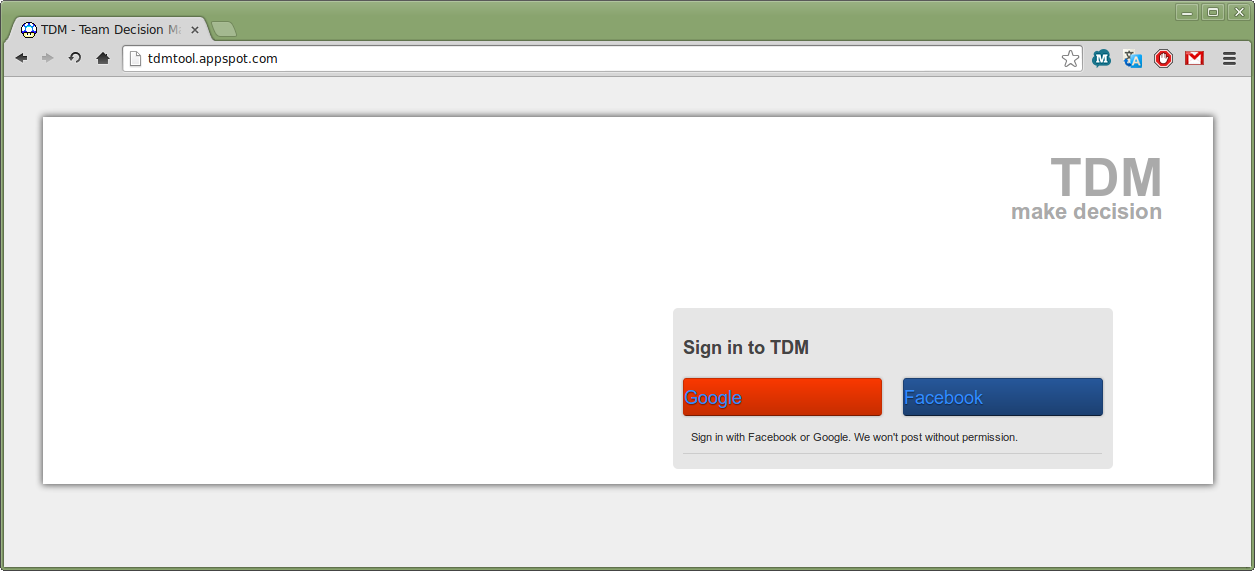
\includegraphics[width=\linewidth]
    {chapters/prototyp/tdm_authentication}
  \caption{Autentykacji do aplikacji TDM}
  \label{fig:authentication}
\end{figure}

\subsubsection{Lista problemów}
\begin{figure}[!htbp]
  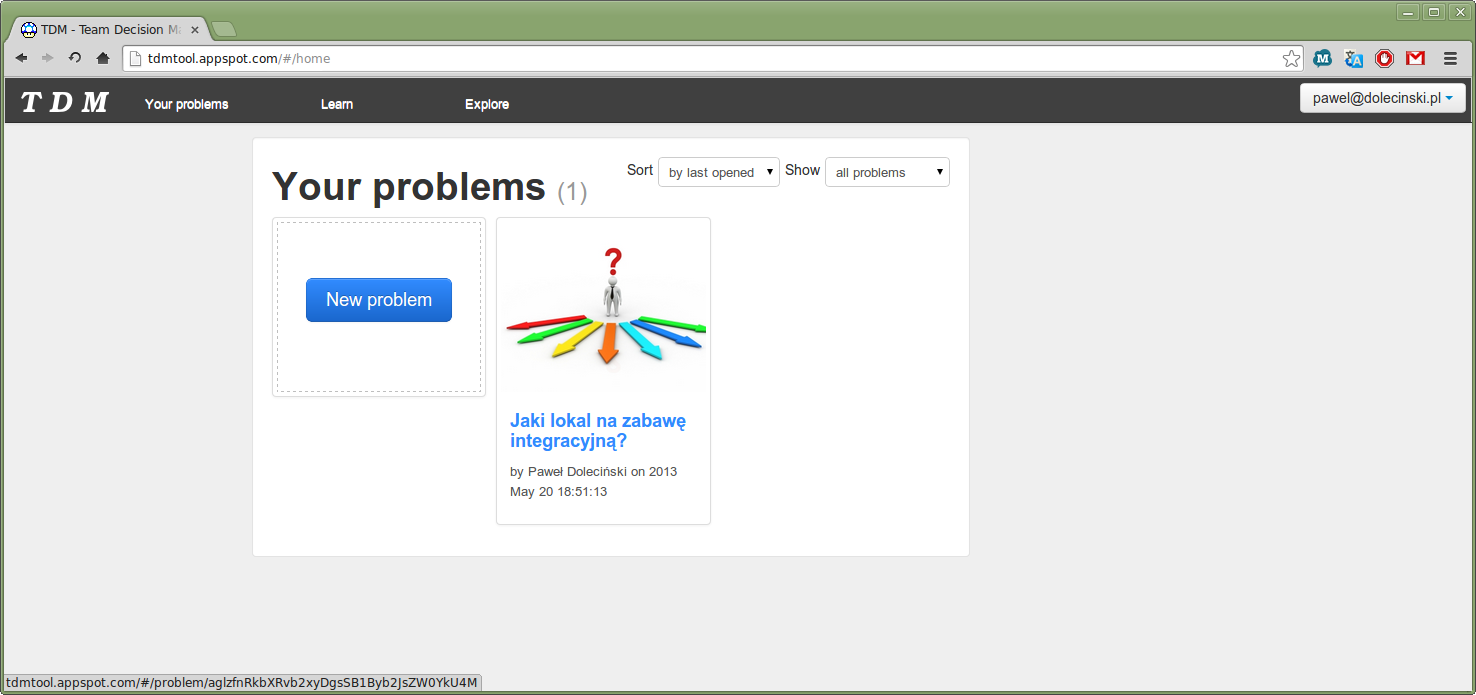
\includegraphics[width=\linewidth]
    {chapters/prototyp/tdm_problem_list}
  \caption{Lista aktualnych problemów decyzyjnych}
  \label{fig:problem_list}
\end{figure}

Po zalogowaniu użytkownik zobaczy ekran z dostępną listą problemów decyzyjnych
do rozwiązania. W tym miejscu widać elementy stworzone przez zalogowanego
eksperta oraz te, do których został zaproszony. Na tym ekranie można również
rozpocząć całkowicie nowy proces decyzyjny poprzez wybranie opcji ,,New
problem''. Wyświetlone zostanie okno dialogowe z prośbą o podanie nazwy problemu
oraz jego opcjonalnego opisu (rysunek \ref{fig:new_problem}). Jak widać,
aplikacja stara się jak najbardziej uprościć proces, a tym samym go
przyspieszyć. Stąd wszystkie techniczne parametru opisu problemu przyjmują
optymalne dla większości przypadków wartości domyślne z możliwością późniejszej
modyfikacji.

\begin{figure}[!htbp]
  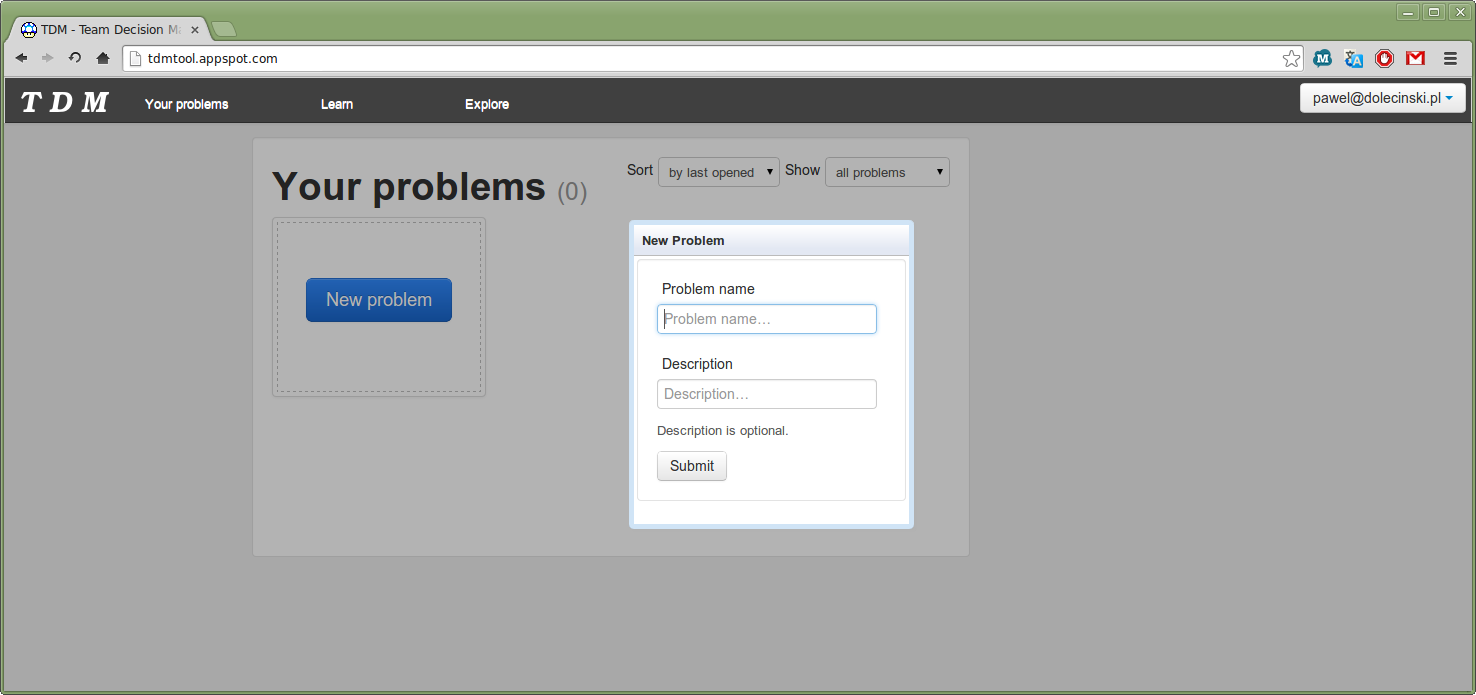
\includegraphics[width=\linewidth]
    {chapters/prototyp/tdm_new_problem}
  \caption{Okno dodawania nowego problemu decyzyjnego}
  \label{fig:new_problem}
\end{figure}

\subsubsection{Burza mózgów}
\begin{figure}[!htbp]
  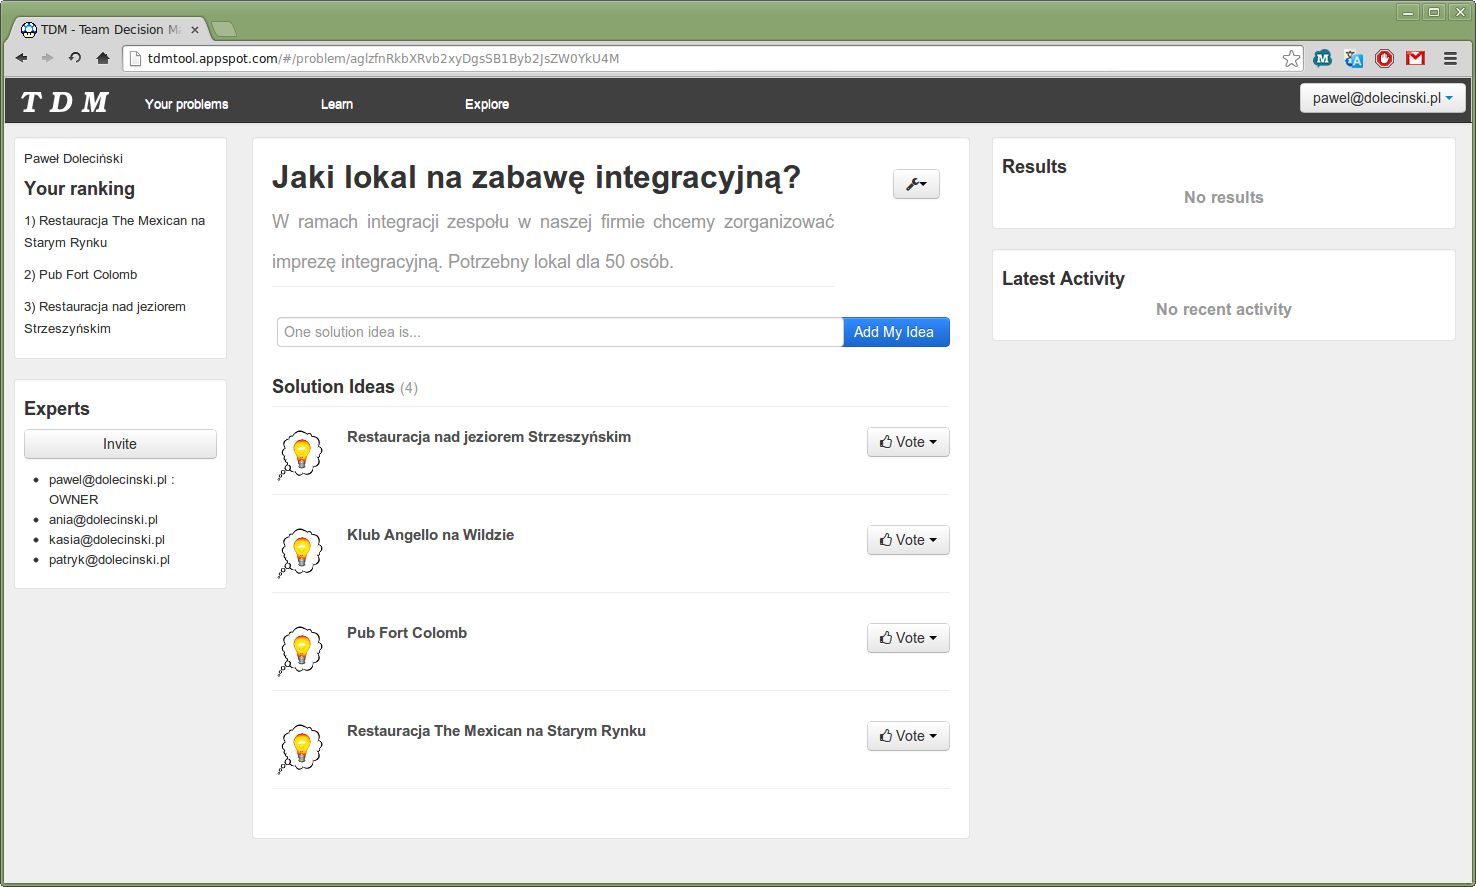
\includegraphics[width=\linewidth]
    {chapters/prototyp/tdm_brainstorm}
  \caption{Burza mózgów}
  \label{fig:brainstorm}
\end{figure}
Centralne miejsce aplikacji. To tutaj odbywa się cała dyskusja. Z poziomu ekranu
problemu decyzjnego jest dostęp do dodawania nowych alternatyw, komentowania,
głosowania. Widać aktualne wyniki oraz powiadomienia systemowe. Każdy z tych
elementów został omówiony bardziej szczegółowo w kolejnych sekcjach.

\subsubsection{Nowa alternatywa}
\missingfigure{Klient: nowa alternatywa}
Dodanie nowej alternatywy ogranicza się do wpisania kilku słów opisu i
naciśnięcia jednego przycisku. Natychmiast po tym propozycja rozsyłana jest do
pozostałych ekspertów, a na ekranie pojawia się dodatkowe okno z możliwością
bardziej szczegółowego przedstawienia swojego pomysłu. Jest tam miejsce na
dyskusję, która jest całkowicie anonimowa. Anonimowe jest też samo dodanie
alternatywy. Zabieg ten pomoga uniknąć ekspertom padnięcia ofiarami opisanego
wcześniej grupowego myślenia.

\subsubsection{Członkowie grupy}
Po lewej stronie widoku z ,,burzą mózgów'' widoczna jest lista wszystkich
uczestników dyskusji, czyli tak zwanych ekspertów. Zawsze jeden z członków grupy
jest wyróżniony. Jest to tak zwany właściciel, czyli osoba która stworzyła
problem. To do właściciela należy ostatnie słowo, czyli możliwość zakończenia
całego procesu w każdej chwili. Na liście członków grupy pokazywana jest też
aktualna dostępność każdej osoby.

Zaproszenie nowych ekspertów sprowadza się do podania adresów e-mail oraz kilku
słów zachęty. Na każdy z podanych adresów zostanie wysłana wiadomość e-mail z
zaproszeniem do udziału w dyskusji wraz z adresem dostępu. Wejście na podany
adres wymaga od użytkownika jedynie zalogowania do systemu, po czym od razu
możliwe jest uczestnictwo w procesie decyzyjnym.
\begin{figure}[!htbp]
  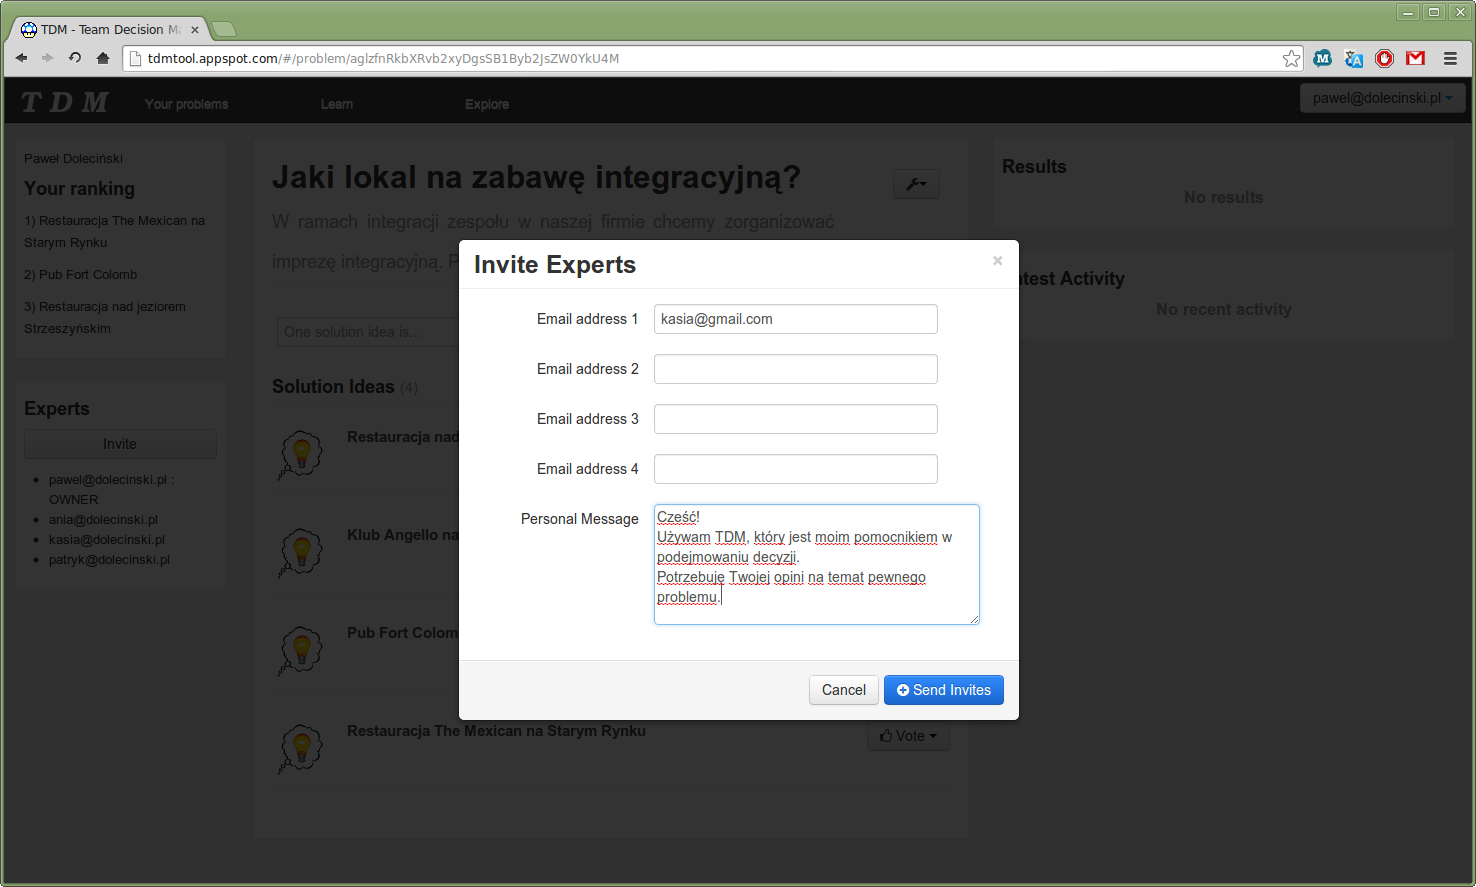
\includegraphics[width=\linewidth]
    {chapters/prototyp/tdm_invitation}
  \caption{Zapraszanie ekspertów}
  \label{fig:invitation}
\end{figure}
\missingfigure{Klient: głosowanie}
\subsubsection{Głosowanie i wyniki}
Ostatnim ważnym elementem prototypu klienta aplikacji TDM jest możliwość
wprowadzania swoich preferencji względem zaproponowanych alternatyw oraz,
prezentowane po prawej stronie widoku ,,burzy mózgów'', statystyki głosowań i
rekomendowane przez system rozwiązanie optymalne dla grupy.

\subsection{Serwer}
Serwer to serce projektu i jednocześnie podstawowa implementacja modelu systemu
grupowego podejmowania decyzji przedstawionego w poprzednim rozdziale. 

Całość zaimplementowana w języku Java i Scala, w oparciu o technologię JavaEE
oraz Spring Framework. Aplikacja TDM została wdrożona na Google App Engine,
platformie działającej jako chmura obliczeniowa udostępniona na
zasadzie platforma jako usługa (PaaS, ang. platform as a service).

Architektura serwera może być przedstawiona na dwa sposoby. Pierwszy to podział
na moduły logiczne odpowiadające modułom modelu teoretycznego. Drugi to podział
na warstwy przepływu danych oraz moduły odpowiedzialne za pracę w każdej z warstw.

\subsubsection{Moduły logiczne}
Przed szczegółowym opisem modułów warto wspomnieć, że użytkownik po wysłaniu
swoich preferencji nie czeka na odpowiedź serwera. Może kontynuować dyskusję,
zgłaszać nowe pomysły rozwiązań, a nawet wysłać nowe preferencje. Serwer sam
poinformuje o nowych wynikach głosowania jak tylko będzie gotowy. Dzięki temu
zachowana jest dynamika i naturalność dyskusji oraz całego procesu. Wszystkie
komunikaty wysyłane do serwera oraz zwracane przez serwer są całkowicie
asynchroniczne.

\begin{itemize}
  \item \emph{Moduł unifikowania preferencji}. Jest odpowiedzialny za
  zunifikowanie preferencji nadesłanych przez ekspertów przy użyciu funkcji
  transformacji zaproponowanych w modelu teoretycznym. Co prawda prototyp
  klienta TDM pozwala podać preferencje tylko przy pomocy funkcji użyteczności,
  jednak serwer w pełni obługuje wszystkie cztery możliwości oceny alternatyw.
  Ze względu na funkcyjną postać transformacji, cały moduł został
  zaimplementowany w języku Scala z rodziny języków dla maszyny wirtualnej Javy,
  który wspiera paradygmat programawania funkcyjnego. Zunifikowane preferencje
  zapisywane są w bazie danych lub, jeżeli dany użytkownik głosował już, to dane
  w bazie są nadpisywane bądź uzupełniane.

  \item \emph{Moduł selekcji}. Zaraz po zunifikowaniu ocen ekspertów, serwer
  przechodzi do fazy selekcji, czyli próby wyznaczenia najlepszego w danej
  chwili rozwiązania. Wyniki obliczeń propagowane są wśród wszystkich
  podłączonych w danym momencie aplikacji klienckich oraz zapisywana w bazie
  danych. Dodatkowo w bazie zapisywane są pośrednie wyniki, czyli zagregowana
  relacja preferencji oraz stopnie dominancji.

  \item \emph{Moduł konsensusu}. Zgodnie z metodami obliczeń z modelu
  sprawdzany jest poziom konsensusu grupy. Innymi słowy, ten fragment serwera
  odpowiedzialny jest za poinformowanie użytkowników czy mogą zakończyć
  dyskusję, czy jeszcze nie. Przeciwnie do innych systemów grupowego
  podejmowania decyzji, serwer TDM nie kończy całego procesu i nie podaje
  finalnego rozwiązania w przypadku osiągnięcia minimalnego poziomu konsensusu.
  Rozsyłana jest jedynie informacja, że taki poziom został osiągnięty wraz z
  sugestią zakończenia. Każdorazowo moduł rozsyła także statystyki dotyczące
  głosowań, czyli ilu z zaproszonych ekspertów wyraziło swoje zdanie i w jakim
  stopniu to zdanie jest kompletne.

  \item \emph{Moduł informacji zwrotnej}. Jeżeli nie został osiągnięty minimalny
  poziom konsesusu, to moduł ten będzie się starał ,,pchnąć'' użytkowników w
  stronę osiągnięcia tego poziomu. Na podstawie danych zebranych w poprzednich
  modułach generowane są rekomendacje dla eksperta, który nadesłał preferencje.
  O ile moduł selekcji i moduł konsensusu rozsyłają wyniki obliczeń do
  wszystkich aktywnych użytkowników, o tyle moduł informacji zwrotnej wysyła
  rekomendacje jako odpowiedź na nadesłane preferencje.

  \item \emph{Moduł zarządzania problemami}. Część systemu niewchodząca w skład
  samego modelu teoretycznego, jednak niezbędna do pracy całości. Jest to moduł
  odpowiedzialny za tworzenie, pobieranie, archwizację problemów. 
   
\end{itemize}
\subsubsection{Architektura trójwarstwowa}
Architektura trójwarstwowa (ang. three-tier architecture) to koncepcja, w której
interfejs użytkownika, przetwarzanie danych i składowanie danych są rozwijane w
postaci osobnych modułów. Prototyp serwera TDM jest zaimplementowany właśnie w
taki sposób.

\begin{description}
  \item[Warstwa interfejsu użytkownika] (ang. presentation
  layer) zaimplementowana z użyciem biblioteki Spring MVC jest odpowiedzialna za
  bezpośrednią komunikację z klientem.
  Nasłuchuje na żądania, po wstępnej walidacji i transformacji przesyła dane do
  niższej warstwy. Komunikacja przebiega tak samo w drugą stronę, to znaczy
  kiedy warstwa logiki aplikacji posiada dane dla klienta, to warstwa interfejsu
  użytkownika odpowiada za wysłanie tych danych. Na tym poziomie zdefiniowany
  jest protokół komunikacji REST oraz serializacja/deserializacja obiektów
  języka Java do formatu JSON (ang. JavaScript Object Notation).
  
  \item[Warstwa przetwarzania danych] zwana inaczej warstwą logiki biznesowej
  (ang. business logic layer). Opisane wcześniej moduły logiczne
  zaimplementowane są właśnie na tym poziomie. Jest to warstwa, która skupia się
  na samym modelu i logice bez wchodzenia w szczegóły techniczne wykorzystywanej
  technologii. Dzięki temu w każdym momencie możliwa jest łatwa zmiana protokołu
  komunikacji z klientem albo zmiana wykorzystywanej bazy danych lub serwera.
  Łatwiejsze i wygodniejsze jest także testowanie samego modelu.
  
  \item[Warstwa składowania danych] zwana inaczej warstwą persystencji (ang.
  persistance layer). Najniższa warstwa, odpowiedzialna za zapis wyników
  obliczeń i danych pochodzących z warstwy logiki biznesowej. Prototyp TDM z
  uwagi na wykorzystanie Google App Engine, korzysta z obiektowej bazy danych
  zamiast tradycyjnej relacyjnej, co daje elastyczny i łatwo rozszerzalny
  schemat bazy. Jednocześnie nie jest potrzebna bezpośrednia komunikacja z bazą
  danych, ponieważ został użyty standard persystencji obiektów Javy JDO (ang.
  Java Data Objects), który jest niezależny od dostawcy wykorzystywanej bazy.
\end{description}
Jak widać, cały serwer jest bardzo mocno zmodularyzowany, co pozwala na duże
możliwości rozszerzania o nowe funkcjonalności oraz w przyszłości zmiany
wykorzystywanych technologii na nowsze.

\section{Studium przypadku}
W tym podrozdziale zilustrowany jest prosty, ale prawdziwy przykład
wykorzystania systemu wpierania decyzji grupowej. Warto zwrócić uwagę na
zachowanie systemu w przypadku złożonych problemów, kiedy to zbiór alternatyw
może bardzo się zmieniać w krótkich odstępach czasu, jak również zbiór ten może
być bardzo duży. Model systemu nie nakłada żadnych ograniczeń ilościowych na
alternatywy, może też obsługiwać dowolną liczbę ekspertów. Aby pokazać działanie
prototypu, będziemy śledzić przepływ informacji przedstawiony wcześniej.

Jako studium przypadku została wybrana grupa czterech osób - współpracowników,
którzy muszą wybrać lokal na spotkanie integracyjne. Wszyscy na co dzień
pracują w różnych krajach i w różnych strefach czasowych, co uniemożliwia
wspólne spotkanie w celu dokonania wyboru.

W pierwszej kolejności jeden z członków grupy (zwany dalej moderatorem) musi
stworzyć nowy problem w aplikacji TDM. Trzeba podać nazwę problemu oraz
opcjonalalnie opis wyjaśniający problem. Następnie, aby proces miał sens, trzeba
podać przynajmniej dwie alternatywy oraz zaprosić do dyskusji pozostałe osoby. W
tym przykładzie na początku dostępnych jest pięć propozycji lokali zebranych w
tabeli \ref{tab:init_ideas}.
\missingfigure{screenshot z aplikacji: dodanie idei oraz ekspertow}
Aplikacja samodzielnie inicjalizuje niezbędne dla obliczeń parametry problemu
decyzyjnego. Samodzielnie można zmienić maksymalny podzbiór alternatyw brany pod
uwagę, który domyślnie przyjmuje wartość nieskończoną. Dla prostoty przykładu
oraz lepszego pokazania dynamiki alternatyw maksymalny podzbiór alternatyw
ustawiony jest na 4. Wszystkie wartości parametrów zebrane zostały w tabeli
\ref{tab:init_problem_params}.

\begin{table}[ht]
\caption{Początkowe propozycje rozwiązania problemu}
\begin{tabularx}{\textwidth}{|c|c|X|}
\hline
ID & Nazwa & Opis \\
\hline
$x_1$ & Lokal 1 & Miejsca: $75$ Cena: $100\textrm{zł}$ \\
\hline
$x_2$ & Lokal 2 & Miejsca: $50$ Cena: $90\textrm{zł}$ \\
\hline
$x_3$ & Lokal 3 & Miejsca: $60$ Cena: $120\textrm{zł}$ \\
\hline
$x_4$ & Lokal 4 & Miejsca: $100$ Cena: $60\textrm{zł}$ \\
\hline
$x_5$ & Lokal 5 & Miejsca: $75$ Cena: $70\textrm{zł}$ \\
\hline
\end{tabularx}
\label{tab:init_ideas}
\end{table}

\begin{table}[ht]
\caption{Początkowe parametry problemu}
\begin{tabularx}{\textwidth}{|c|c|X|}
\hline
Nazwa & Wartość & Opis \\
\hline
b & 1 & Kontroluje rygorystyczność procesu przy obliczaniu miar bliskości \\
\hline
$\beta$ & 0.5 & kontroluje zachowanie OR-LIKE operatora agregacji \\
\hline
minConsDegree & 0.8 & Minimalny poziom konsensusu \\
\hline
minProxDegree & 0.7 & Minimalny poziom bliskości \\
\hline
minQGDD & 0.2 & Minimalny poziom dominancji \\
\hline
DSsize & 4 & Maksymalny podzbiór alternatyw \\
\hline
\end{tabularx}
\label{tab:init_problem_params}
\end{table}

Należy zwrocić uwagę, że początkowy zbiór wszystkich rozwiązań składa się z
pięciu lokali $\mathcal{X} = \{ x_1, x_2, x_3, x_4, x_5\}$, natomiast założono,
że eksperci powinni w jednym momencie skupić się na ocenie maksymalnie czterech.
Zatem początkowy podzbiór rozwiązań składa się tylko z pierwszych czterech
zaproponowanych $\mathcal{X'} = \{ x_1, x_2, x_3, x_4\}$.

Dla uproszczenia obliczeń oraz ze względu na ograniczoną ilość miejsca w tej
pracy, pokazane zostaną tylko dwie ,,rundy''. Zakładamy też, że każda runda na
wejściu otrzymuje kompletny zbiór preferencji od każdego z ekspertów. 
Warto natomiast pamiętać, że cały proces uruchamiany jest każdorazowo dla
pojedynczego głosu. 

\subsection{Pierwszy etap w procesie decyzyjnym}
Na rysunku pokazane są preferencje ekspertów wyrażone za pomocą funkcji
użyteczności.

\subsubsection{Etap unifikowania}
W pierwszej kolejności preferencje podane przez ekspertów muszą zostać poddane
unifikacji, czyli wyrażone za pomocą rozmytej relacji preferencji. Moduł
unifikowania wykorzystuje wzory transformacji opisane w modelu teoretycznym, co
daje następujące wyniki:
$$
P^1 = 
\begin{pmatrix}
0.5  & 0.16  & 0.33  & 0    \\
0.83 & 0.5   & 0.66  & 0.33 \\
0.66 & 0.33  & 0.5   & 0.16 \\
1    & 0.66  & 0.83  & 0.5
\end{pmatrix},\;
P^2 = 
\begin{pmatrix}
0.5  & 0.57  & 0.88  & 0.94 \\
0.43 & 0.5   & 0.84  & 0.92 \\
0.22 & 0.16  & 0.5   & 0.69 \\
0.06 & 0.08  & 0.21  & 0.5
\end{pmatrix},
$$

$$
P^3 = 
\begin{pmatrix}
0.5  & 0.3   & 0.9   & 0.7  \\
0.7  & 0.5   & 1     & 0.8  \\
0.1  & 0     & 0.5   & 0.2  \\
0.3  & 0.2   & 0.8   & 0.5
\end{pmatrix},\;
P^4 = 
\begin{pmatrix}
0.5  & 0.66  & 0.97  & 0.82 \\
0.34 & 0.5   & 0.91  & 0.66 \\
0.03 & 0.09  & 0.5   & 0.18 \\
0.18 & 0.34  & 0.82  & 0.5
\end{pmatrix}.
$$
  
\subsubsection{Proces selekcji}
Wykorzystując kryterium rozmytej większości oraz operator OWA z wektorem wag
$W= [0.5,0.2,0.17,0.13]$ (,,większość''), w fazie agregacji obliczana jest
zbiorowa rozmyta relacja preferencji:
$$
P^c = 
\begin{pmatrix}
0.5  & 0.52  & 0.86   & 0.7  \\
0.48 & 0.5   & 0.91   & 0.8  \\
0.14 & 0.09  & 0.5    & 0.2  \\
0.25 & 0.23  & 0.56   & 0.5
\end{pmatrix}.
$$

Następnie moduł eksploatacji przedstawi proponowane rozwiązanie problemu. 
W oparciu o operator OWA z wektorem wag $W = [0.07, 0.67, 0.26]$
(,,większość'') obliczane są stopnie dominancji (QGDD): $QGDD_1 = 0.696$,
$QGDD_2 = 0.702$, $QGDD_3 = 0.146$, $QGDD_4 = 0.265$. Są to wartości, które
reprezentują dominancje jaką jedna alternatywa ma nad ,,większością''
pozostałych alternatyw według ,,większości'' ekspertów.

Na podstawie powyższych wyników widać, że obecnie najlepszym kandydatem jest
lokal drugi $x_2$, a tymczasowe rozwiązanie można zaprezentować jako
uporządkowaną listę $\{ x_2, x_1,x_4, x_3\}$.

\subsubsection{Proces konsensusu}
Pierwszy krok został już osiągniety. System może przedstawić proponowane
rozwiązanie na podstawie zgłoszonych preferencji ekspertów. Ale to nie koniec. W
module konsensusu system musi sprawdzić w jakim stopniu eksperci są zgodni ze
sobą, tzn. czy zaproponowane wyżej rozwiązanie jest rozwiązaniem odpowiadającym
większości grupy.

Najpierw moduł musi ustalić indywidualne dla każdego eksperta uporządkowanie
alternatyw na tej samej zasadzie, co obliczanie zbiorczego rozwiązania:
$$e_1: \{ x_4, x_2, x_3, x_1 \}, \;\; e_2: \{ x_1, x_2, x_3, x_4 \},$$
$$e_3: \{ x_1, x_2, x_4, x_3 \}, \;\; e_4: \{ x_2, x_1, x_4, x_3 \}.$$

Stopnie konsensusu dla każdej z alternatyw to: $C(x_1) = 0.55, C(x_2) =
0.66,$ $C(x_3) = 0.77, C(x_4) = 0.66.$ Miara konsensusu wynosi
$C_{\mathcal{X}} = 0.67$.
Ostatecznie obliczone miary bliskości wynoszą: $P^1_{\mathcal{X}} = 0.55,\;
P^2_{\mathcal{X}} = 0.67,\; P^3_{\mathcal{X}} = 0.78,\; P^4_{\mathcal{X}} = 1$.

Jasno widać, że konsensus nie osiągnął wymaganej wartości minimalnej
($C_{\mathcal{X}} < 0.8$), czyli aplikacja powinna kontynuować kolejne etapy,
szczególnie etap generowania informacji zwrotnej.

\subsubsection{Dynamiczny wybór alternatyw}
Eksperci w każdym momencie działania aplikacji mogą zgłaszać nowe alternatywy,
mogą również zgłosić, że jedna z opcji brana do tej pory pod uwagę jest już
nieaktualna, na przykład jeden z lokali ma już komplet rezerwacji.
W tej sytuacji niezbędna jest aktualizacja wszystkich danych o problemie, które
mogły się zmienić w trakcie działania procesu.

W tym przypadku okazało się, że alternatywa $x_3$ nie osiągnęła minimalnego
stopnia dominancji, t.j. $QGDD_3 < MinQGDD = 0.2$. W międzyczasie zgłoszona
została nowa propozycja $x_6$. System zgłasza usunięcie $x_3$ z
podzbioru dyskusji oraz dołączenie w to miejsce $x_6$. Jest jeszcze jedna
oczekująca alternatywa $x_5$, jednak aplikacja w pierwszej kolejności promuje
najnowsze propozycje ekspertów. W przypadku większej ilości propozycji istnieje
możliwość wstępnego głosowania na nowe opcje. Inną możliwością jest zwiększenie
rozmiaru podzbioru dyskusji.

\subsubsection{Informacja zwrotna}
Moduł informacji zwrotnej jest odpowiedzialny za doprowadzanie grupy do jak
największego konsensusu. Zatem generowane są rekomendacje oraz podpowiedzi dla
każdego członka, który nie zgadza się z większością. Oczywiście są to tylko
wskazówki, których nie trzeba stosować.

Aplikacja najpierw szereguje ekspertów według osiągniętych przez nich miar
bliskości: $e_4, e_3, e_2, e_1$. W tym momencie widać, że dwóch członków grupy,
$e_2$ i $e_1$, uzyskało poziom bliskości poniżej minimalnego $minProxDegree$,
zatem oni zostaną poproszeni o zmianę swoich preferencji. Oczywiście
rekomendacje na temat propozycji $x_3$ są pomijane ze względu na jej usunięcie.
Natomiast wszyscy eksperci są proszeni o podanie swoich preferencji dla nowej
alternatywy $x_6$. Rekomendacje otrzymane przez ekspertów można zobaczyć na
rysunku. \missingfigure{Rekomendacje dla ekspertów}

\subsection{Drugi etap w procesie decyzyjnym}
Jest to faza, w której wszyscy eksperci ponownie wysłali swoje preferencje dla
wszystkich alternatyw w oparciu o rekomendacje. Wszystkie preferencje zostały
zebrane na rysunku. \missingfigure{Rekomendacje dla ekspertów}

Cały proces z rundy pierwszej jest powtarzany, tzn. preferencje są
transformowane do rozmytych relacji preferencji, a moduł selekcji przedstawia
nowe rozwiązanie problemu. Nowy ranking lokali to $x_2, x_1, x_6, x_4$.

Następnie moduł konsensusu sprawdza osiągnięty poziom porozumienia. Dla podanych
danych przykładowych otrzymano $C_{\mathcal{X}} = 0.88$. Oznacza to, że został
osiągnięty minimalny poziom wymagany przez problem ($C_{\mathcal{X}} > 0.8$),
a grupa zostaje zapoznana z proponowanym rozwiązaniem. Aplikacja informuje, że
większość członków grupy zgadza się ze sobą, ale nic nie stoi na przeszkodzie w
kontynuowaniu dyskusji - decyzja zawsze należy do grupy.

	
	\chapter{Podsumowanie i plany rozwoju systemu}
	W niniejszej pracy zostało przedstawione szeroko pojęte wspieranie podejmowania
decyzji grupowej w warunkach dynamicznych. Obecnie często brakuje
czasu na spotkanie w cztery oczy i prowadzenie długich dyskusji. Co więcej,
natłok informacji oraz jej częsta dezaktualizacja dodatkowo utrudnia cały
proces. Stąd wsparcie ze strony technologii może okazać się bardzo przydatne.

Na początku wprowadzony został ogólny wstęp do teorii decyzji oraz do teorii
grupowego podejmowania decyzji. Zostały naświetlone trudności z jakimi boryka
się grupa decyzyjna, takie jak dysonans poznawczy, iluzje decyzyjne, czy
największy problem - syndrom grupowego myślenia. Są to wyzwania dla systemu
wspierającego grupowe podejmowanie decyzji, o których większość modeli
teoretycznych zapomina. Wszystkie te trudności wynikają z prowadzenia dyskusji,
czyli głównego elementu procesu.

W ramach pracy zaprezentowany został model teoretyczny procesu decyzyjnego
wykorzystujący narzędzia logiki rozmytej. Jedną z jego głównych zalet jest
zrezygnowanie z podejścia iteracyjnego na rzecz większej dynamiki oraz
naturalności procesu. Eksperci mają też dużą swobodę w sposobie wyrażania swoich
preferencji względem dostępnych alternatyw.

Jako dowód koncepcji (ang. proof of concept) zaimplementowany został prototyp
systemu TDM realizujący główne założenia przedstawione w pracy. Jest to
aplikacja internetowa oparta o najnowsze technologie, co zapewnia dostępność
systemu dla dużej ilości urządzeń, w tym mobilnych. Zaprojektowana
architektura pozwala na dużą rozszerzalność systemu, na przykład łatwe
stworzenie natywnych aplikacji klienckich na telefony komórkowe. Centralnym
miejscem jest ekran tak zwanej ,,burzy mózgów'', a zadaniem oprogramowania jest
wspieranie grupy, nakierowywanie na osiągnięcie konsensusu oraz rekomendowanie
rozwiązań. Natomiast celem nie jest zastąpienie grupy i podejmowanie decyzji za
ekspertów. Zakres projektu nie obejmuje pełnego modelu, a jedynie główne
koncepcje. Dla przykładu, ocenianie alternatyw możliwe jest tylko za pomocą
jednej spośród wszystkich opisanych metod.

Plany dalszego rozwoju aplikacji TDM obejmują:
\begin{itemize}
  \item implementację autorskiej metody zarządzania dynamiką zbioru alternatyw,
  \item bardziej intuicyjny sposób prezentacji statystyk głosowania oraz
  proponowanego rozwiązania problemu,
  \item implementację wszystkich opisanych w pracy metod wprowadzania
  preferencji, w tym także oceny lingwistycznej,
  \item integrację z szeroką gamą serwisów społecznościowych.
\end{itemize}
Wszystkie powyższe elementy mają na celu ułatwienie i usprawnienie pracy
użytkownika, a przez to skuteczniejsze podejmowanie decyzji i rozwiązywanie
problemów przez grupę ekspertów.


	
	
    \nocite{*}
    \label{biblio}
    \bibliographystyle{bib/plain_pl}
    \bibliography{bib/bibliography}
    \newpage
    \addtolength\cftfigurenumwidth{1em} % Większy odstęp pomiedzy numerem rys. a jego tytułem.
    \listoffigures
	\newpage
	\addtolength\cfttablenumwidth{1em}
	\listoftables	
	
	\begin{comment}
    \label{Załączniki}
    \newpage
    \appendix
    \renewcommand{\appendixtocname}{Załączniki}
    \renewcommand{\appendixpagename}{~\vspace{8cm} \begin{center}Załączniki\end{center}\newpage}
    \thispagestyle{empty}
    \addappheadtotoc
    \appendixpage
	\end{comment}

	\listoftodos
\end{document}
